\documentclass[12pt, a4paper]{report}
\usepackage[utf8]{inputenc}
\usepackage{amsmath}
\usepackage{amsfonts}
\usepackage{amssymb}
\usepackage{graphicx}
\usepackage[left=2.5cm,right=2.5cm,top=2cm,bottom=2cm]{geometry}
\usepackage{wrapfig}
%\usepackage{subfigure}
\usepackage{blindtext}
\usepackage{tabularx}
\usepackage{epsfig}
\usepackage{epstopdf}
\usepackage[space]{grffile}
\usepackage[nottoc]{tocbibind}
\usepackage{color}
\usepackage{gensymb}
\usepackage{textgreek}
\usepackage{textcomp}
\usepackage{xcolor}
\usepackage{listings}
\usepackage{subcaption}
\usepackage{tocloft,calc}
\usepackage{float}
%\usepackage{polski}
\usepackage[utf8]{inputenc}
\usepackage[T1]{fontenc}
\usepackage{lmodern}

\usepackage{afterpage}
\newcommand\blankpage{%
    \null
    \thispagestyle{empty}%
    \addtocounter{page}{-1}%
    \newpage}

\renewcommand{\cftchappresnum}{Chapter }
\AtBeginDocument{\addtolength\cftchapnumwidth{\widthof{\bfseries Chapter }}}

\linespread{1.5}

\author{Paweł Palczyński}
\title{Physical Characterization of Atomically-Thin Transition Metal Dichalcogenides}

\DeclareUnicodeCharacter{2212}{-}

%%%%%%%%%%%%%%%%%%%%%%%%%%%%%%%%%%%%%%%%%%%%%%%%%%%%%%%%%%%%%%%%%

\begin{document}

\begin{titlepage}
	\begin{center}
		\begin{Large}
		\vspace*{4cm}
		
		\textbf{Characterisation of Atomically-Thin Transition Metal Dichalcogenides}\\
		\vspace{0.5cm}
		\end{Large}
		
		\vspace{0.5cm}
		by\\
		\vspace{0.5cm}
		\large{\textbf{Paweł Jan Palczyński}}
		\vspace{0.5cm}
		
		\small{A thesis submitted in partial fulfilment of the requirements for the award of the degree}\\
		\vspace{0.5cm}
		\begin{normalsize}
		\large{Doctor of Philosophy}\\
		\end{normalsize}
		\vspace{0.5cm}
		from\\
		\vspace{0.5cm}
		\large{Imperial College London}\\
		\vfill
		Faculty of Engineering, Department of Materials\\
		\today
	\end{center}
\end{titlepage}
\newpage \blankpage
\section*{Declaration of originality}

I hereby declare that this thesis is the result of my own work unless otherwise referenced or acknowledged. This document is submitted in partial fulfilment of the requirements for the award of Doctor of Philosophy in the Department of Materials, Imperial College London and it has not been submitted to any other academic institution awarding qualifications.\\ \\

Paweł Jan Palczyński
\section*{Copyright declaration}

"The copyright of this thesis rests with the author. Unless otherwise indicated, its contents are licensed under a Creative Commons
Attribution-Non Commercial 4.0 International Licence (CC BY-NC). Under this licence, you may copy and redistribute the material in any
medium or format. You may also create and distribute modified versions of the work. This is on the condition that: you credit the
author and do not use it, or any derivative works, for a commercial purpose.
When reusing or sharing this work, ensure you make the licence terms clear to others by naming the licence and linking to the licence
text. Where a work has been adapted, you should indicate that the work has been changed and describe those changes.
Please seek permission from the copyright holder for uses of this work that are not included in this licence or permitted under UK
Copyright Law."
\section*{Acknowledgements}

I would like to thank my supervisor Dr. Cecilia Mattevi for enormous amount of help, guidance, support and patience throughout my entire time in her group. 

I would also like to acknowledge the examiners, Prof. Alexander Tartakovskii and Dr Peter Petrov for reviewing this thesis.

Thank you to Dr Francesco Reale for all the talks, both serious and lighthearted, and for providing me with all the CVD samples, XRD, SEM and AFM measurements and analysis.

Thank you to Ms Maria Sokolikova for the enlightening conversations and cheering me on to finish this thesis, and for all the colloidal synthesis samples, TEM imaging and analysis.

Thank you to Dr Peter Sherrell, Dr Federico Pesci and Dr Sharda Kanudha for all the guidance and help with setting up experiments and support, and for heterostructure samples, SEM imaging, electrical measurements and analysis.

I would like to acknowledge the help from collaborators, Dr. Iddo Amit, Prof. Monica F. Craciun and Prof. Saverio Russo for performing the electrical measurements.

Thank you to all the lab and office mates, Chiara Grotta, Cong Lu, Aleksandra Krajewska, Julian Buchinger, Jerome Nicolas, Nikesh Patel, Elisa Burbaum, Jeremy Tan, Mauro Och, Apostolos Panagiotopoulos, Gang Cheng, Giulia Zemignani, Stefano Tagliaferri, Gianmaria Matrone, David Poussin, Shengyang Chen, Luca Occhi, Francesco Salerno, Bartosz Barzdajn for all the interactions, talks and support that made this PhD journey complete.

And finally a thank you to my family, mamie, tacie, bratu i bratowej, for all the love and support, dzi\k{e}kuj\k{e}.
\section*{Publications}

Federico M. Pesci, Maria S. Sokolikova, Chiara Grotta, Peter C. Sherrell, Francesco Reale, Kanudha Sharda, Na Ni, \textbf{Pawel Palczynski}, and Cecilia Mattevi. $MoS_2/WS_2$ heterojunction for photoelectrochemical water oxidation. ACS Catalysis, 7(8):4990-4998, July 2017.\\ \\
Chiara Grotta, Peter C Sherrell, \textbf{Pawel Palczynski}, Maria Sokolikova, Kanudha Sharda, and Cecilia Mattevi. 3D printing of 2D atomically thin materials. ArXiv, 3:8655-8662, October 2017.\\ \\
Francesco Reale, \textbf{Pawel Palczynski}, Iddo Amit, Gareth F. Jones, Jake D. Mehew, Agnes Bacon, Na Ni, Peter C. Sherrell, Stefano Agnoli, Monica F. Craciun, Saverio Russo, and Cecilia Mattevi. High-mobility and high-optical quality atomically thin $WS_2$. Scientific Reports, 7(1), November 2017.\\ \\
T. Wakamura, F. Reale, \textbf{P. Palczynski}, S. Gu\'{e}ron, C. Mattevi, and H. Bouchiat. Strong anisotropic spin-orbit interaction induced in graphene by monolayer $WS_2$. Physical Review Letters, 120(10), March 2018.\\ \\
Hugo Henck, Zeineb Ben Aziza, Debora Pierucci, Feriel Laourine, Francesco Reale, \textbf{Pawel Palczynski}, Julien Chaste, Mathieu G. Silly, Fran\c{c}ois Bertran, Patrick Le F\`{e}vre, Emmanuel Lhuillier, Taro Wakamura, Cecilia Mattevi, Julien E. Rault, Matteo Calandra, and Abdelkarim Ouerghi. Electronic band structure of twodimensional $WS_2$/graphene van der waals heterostructures. Physical Review B, 97(15), April 2018.\\ \\
Peter C. Sherrell, Kanudha Sharda, Chiara Grotta, Jacopo Ranalli, Maria S. Sokolikova, Federico M. Pesci, \textbf{Pawel Palczynski}, Victoria L. Bemmer, and Cecilia Mattevi. Thickness-dependent characterization of chemically exfoliated $TiS_2$ nanosheets. ACS Omega, 3(8):8655{8662, August 2018.\\ \\
Maria S. Sokolikova, Peter C. Sherrell, \textbf{Pawel Palczynski}, Victoria L. Bemmer, and Cecilia Mattevi. Direct solution-phase synthesis of 1T' $WSe_2$ nanosheets. Nature Communications, 10(1), February 2019.\\ \\
T. Wakamura, F. Reale, \textbf{P. Palczynski}, M. Q. Zhao, A. T. C. Johnson, S. Gu\'{e}ron, C. Mattevi, A. Ouerghi, and H. Bouchiat. Spin-orbit interaction induced in graphene by transition metal dichalcogenides. Physical Review B, 99(24), June 2019.
\section*{List of abbreviations}

TMDC - Transition metal dichalcogenide\\
CVD - Chemical vapour deposition\\
PL - Photoluminescence\\
SEM - Scanning electron microscopy\\
TEM - Transmission electron microscopy\\
AFM - Atomic force microscopy\\
XRD - X-ray diffraction\\
XPS - X-ray photoelectron spectrscopy\\
VBM - Valence band maximum\\
CBM - Conduction band minimum\\
DFT - Density functional theory\\
EDS - Energy dispersive x-ray spectroscopy\\
LPE - Liquid phase exfoliation\\
FWHM - Full width half maximum\\
MEX - Mechanically exfoliated\\
OM - Optical microscopy
\section*{Abstract}

Transition metal dichalcogenides (TMDC) are a class of materials that has become increasingly popular in the recent years in the wake of discovery of graphene and its surprising properties. Despite being known for decades and being used in its bulk form as a sold lubricant or catalysts their mono and few layer form remained largely unexplored. Indeed when TMDCs are only one or few layers thick their unique optical and electronic properties emerge. In particular group VI TMDCs such as $MoS_2$ or $WS_2$, as their numbers of layers decreases, turn from an indirect to direct bandgap semiconductor with possible applications in visible range optoelectronic and electronic devices. Moreover unique quantum effects such as quantum spin Hall effect, strong spin orbit interactions or topological insulators can be observed in these thin films.

One of the major hurdles standing in the path of further development of those materials is its synthesis. The commonly used methods successfully optimise one of the many desired parameters and therefore new techniques must be developed to provide an improvement across all aspects of the material quality. In order to properly asses those new growths methods metrological studies must equally contribute to the capabilities of rapid assessment of large area flakes and films. To that effect the commonly used Raman and PL are heavily employed throughout in mapping the as grown as well as transferred flakes on multiple different substrates. In a similar fashion the x-ray spectroscopy is utilised to gain insight into the samples chemistry, layer thickness and crystal structure. This triple role of XPS allowed for initial studies of 1T' $WSe_2$ which combined with Raman and PL spectroscopy with supplement of other characterisation techniques provided valuable introspective into its structure and properties.

The overarching goal of the thesis is to develop synthesis techniques for growth of TMDCs primarily via CVD as well as colloidal synthesis in order to reliably produce thin layers with controllable thickness and lateral size. This work focuses on characterisation of the as grown materials using Raman, PL and XPS techniques to assess the quality and reproducibility of the developed synthesis methods.

Additionally in this work the novel synthesis routes for growth of $WS_2$ large area monolayers have been assessed. The as grown samples on top of exhibiting strong PL response showed remarkable, record high electron mobility in mono and bilayer form. A certain degree of optical and electrical properties tunability is also presented in In doped $WS_2$ layers. By combining the growth of monolayers the heterostructures of $MoS_2/WS_2$ are successfully grown on multiple substrates and their quality and structure is carefully investigated.

\tableofcontents

\chapter{Thesis introduction}

The recently popular group of materials called Transition Metal Dichalcogenides (TMDCs) have attracted a great deal of attention following the discovery of graphene. Many of the materials belonging to that group, such as $WS_2$ or $MoS_2$, are semiconducting in nature. As one of the manifestations of this property is a very strong photoluminescence (PL) response observed across many monolayers of the TMDCs. Despite extensive studies into the nature of this photoluminescence response the full understanding remains elusive. The PL spectrum of many of those monolayers is complex and can be a result of many contributions from different phenomena and particles. Besides the main peak resulting from recombination of excitons, other quasi particles such as trions or bi-excitons can contribute to the spectrum at room temperature. Additionally the interactions between the material and the substrate as well as any surface effects, including adparticles, vacancies, defects or strain can alter the observable spectrum. Due to its 2D nature TMDCs are especially influenced by the surface effects. 

TMDCs can also exhibit different polytype structures with most common being 2H and 1T phases. An interesting phenomena can be observed in regards to those polytypes where different phases can change from semiconducting to metallic. Those phases together with structural defects and strain can also affect the electronic structure of the TMDCs and thus influence the formation of many of the photogenerated particles. Many of these interactions are however still at the early stages of understanding. 

There has been many attempts at simulating the electronic structures using computational methods such as DFT. The results however are not always compatible with the observed phenomena and show even great discrepancies between different approaches.

One of the polytypes, the 1T' phase, shows interesting properties such as that of topological insulator. It has however remained understudied, partially due to difficulty in synthesis. There still remains many TMDCs for which 1T' phase has not been demonstrated.

Because the 2D materials inherently lack much volume or mass, many standard characterisation techniques are insufficient and can either result in insufficient resolution or signal to noise ratio or can not be applied at all. Due to this a limited set of characterisation techniques remains viable. Among those, the most useful methods which can enable metrological characterisation are Raman spectroscopy, photoluminescence (PL) spectroscopy and X-ray Photoelectron Spectroscopy (XPS). Those techniques can provide information over large sample areas in relatively short times. In particular Raman and PL spectroscopy allows for fast mapping of areas in the order of tens of millimetre in air without the need of any sample preparation and could potentially extract information about crystallographic phases, strain, density defects, number of layers and interaction between the layers. Nevertheless, Raman and PL studies of mono and few-layered TMDCs are still at the very early stages and there is still very limited knowledge in the correlation between the materials characteristics and position, width and relative intensity of the Raman and PL peaks.  Both these characterization techniques can enable fast scanning rate of large surface areas (mm and cm scale). XPS can be further used to learn about stoichiometry, oxidation states, defects, doping or alloying and it can be correlated with Raman and PL features. The combined physical and chemical characterisation can therefore help to provide insight into the fundamental properties of those materials.

In this thesis some initial work on the interpretation of PL and Raman spectra in CVD grown $WS_2$, doped $WS_2$, $MoS_2/WS_2$ heterostructures has been performed. This work aims at contributing to the ultimate goal of establishing a correlation system between characterisation and materials properties for wafer scale grown mono and few-layered TMDCs in the 2H and 1T/1T’ polytypes. The two most common methods of producing TMDC monolayers for purpose of research is mechanical exfoliation and chemical vapour deposition (CVD). While the former in many cases tends to provide higher quality flakes it does not scale in terms of size and therefore has to be replaced by different, scalable methods. The most popular such method is CVD, with which continuous layers on at least cm scales has been demonstrated. Due to variety of used precursors and synthesis paths the quality and composition of resulting flakes varies and therefore requires an understanding of its effects on the material properties. 

Using this understanding similar techniques have been applied to $MoS_2$ and $MoS_2/WS_2$ vertical heterostructure. This allowed to contribute to greater body of knowledge about the interactions between the layers in heterojunctions and its effect on the opto-electronic properties. Furthermore, we have studied by PL, Raman spectroscopy and XPS the 2H phase of $WSe_2$ and by Raman spectroscopy and XPS the 1T’ phase of $WSe_2$.

Using colloidal synthesis unique floral formations of 1T' $WSe_2$ have been observed for the first time. They have been characterised using Raman spectroscopy and XPS to provide some of the first studies of those phases to correlate structural properties and characterisation features. 
\chapter{The state-of-the-art of group VI transition metal disulphides and diselenides}
\label{sec:Introduction}
	Following the discovery and characterisation of graphene in last decade the focus has been put on other 2D materials. Similar to graphene other bulk layered materials can exist in a monolayer or few layer form. Furthermore these thin layers also exhibit a significant change of properties when number of layers decreases from bulk all the way to monolayer. One of the most popular groups of these materials are transition metal dichalcogenides (TMDC). Their general form is $MX_2$ where M is a transition metal, and X is a chalcogen atom.  

\section{Properties of TMDCs}
	TMDCs in their layered form have been known, studied and utilised for a long time. They can be found commonly in use as stolid-state lubricants or catalysts. About 60 different TMDCs have been studied and characterised with a general formula of X-M-X where a plane of metal atoms (M) is sandwiched between two chalcogen planes (X). Out of those 40 can be considered layered materials where individual layers are strongly bonded in-plane and weakly bonded out-of-plane in between layers. These weak, interlayer, Van der Waals interactions allow to form a bulk material. These bonds are also what allows for those layers to slide on top of one another similarly to other layered materials like graphite. 
	TMDCs consist of two transition metal and single chalcogen atoms covalently bonded. They can be found in 3 distinct structural polytypes: 1T (tetragonal symmetry, octahedral coordination) with single layer per repeat unit, 2H (hexagonal symmetry, trigonal prismatic coordination) with 2 layers per repeat unit and 3R (rhombohedral symmetry, trigonal prismatic coordination) with 3 layers per repeat unit \cite{ElectronicsAndOptoelectronicsOfTwo-dimensionalTransitionMetalDichalcogenides} as can be seen in Figure \ref{fig:TMDCPolytypes}.
	
	\begin{figure}[h]
	\begin{center}
	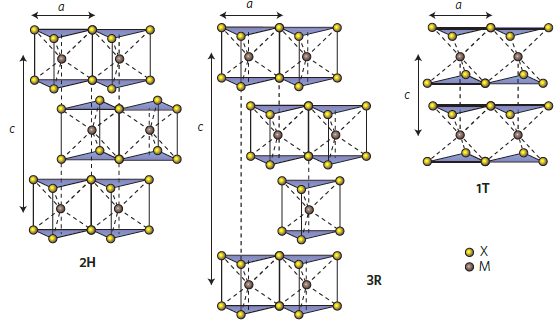
\includegraphics[scale=0.7]{TMDCPolytypes.png}
	\caption{Schematics of the structural polytypes: 2H (hexagonal symmetry, two layers per repeat unit, trigonal prismatic coordination), 3R (rhombohedral symmetry, three layers per repeat unit, trigonal prismatic coordination) and 1T (tetragonal symmetry, one layer per repeat unit, octahedral coordination). The chalcogen atoms (X) are yellow and the metal atoms (M) are grey. The lattice constants a are in the range 3.1 to 3.7 \r{A} for different materials. Adopted from \cite{ElectronicsAndOptoelectronicsOfTwo-dimensionalTransitionMetalDichalcogenides}}
	\label{fig:TMDCPolytypes}
	\end{center}
	\end{figure}
	
	Since graphene have proven to be difficult to work with in the fields of semiconductors due to its lack of natural finite electronic band gap its role as a successor in electronic and opto-electronic devices remains to be seen. However the techniques learned and effects observed during its characterisation were easily transferred to other layered compounds such as TMDCs. In particular the semiconducting, group VI-based TMDCs, containing sulphur and selenium as chalcogen atoms have proven to be more readily potentially useful as an active material in electronic and opto-electronic devices. This is due to their inherent electronic and optical bandgap in visible-near IR range. 
	
	As the number of layers changes from bulk to monolayer the properties of the TMDC undergo a significant change. In most TMDCs the bandgap changes from indirect to a larger direct one. 
	
\subsection{Electronic properties}
	\label{subsec:Electronic properties}
	
	One of the most interesting features that the layered TMDC materials exhibit is the shift in the bandstructure with the changing number of layers. Several studies have shown in simulations and experimentally that TMDCs have very similar electronic band structure as seen in example of $WS_2$ in Figure \ref{fig:WS2BandStructureSimulation}. In bulk $WS_2$ the maximum of the valence band (VBM) at $\Gamma$ point and the minimum of the conduction band (CBM) at $\Lambda$ form an indirect bandgap. As the number of the layers decreases the CBM at $\Lambda$ point as well as VBM at $K$ point increases causing the band gap to widen. At 2 layers the $K$ point becomes the actual CBM and a new indirect bandgap forms between $\Gamma$ point and $K$ point. Finally in a $WS_2$ monolayer the VBM at $K$ point as well as entire conduction band increases to form a new greater direct band gap at $K$ point. This means that $WS_2$ bandgap changes from 1.3 eV indirect bandgap in bulk to 2.1 eV direct bandgap in monolayer.
	
	\begin{figure}[h]
	\begin{center}
	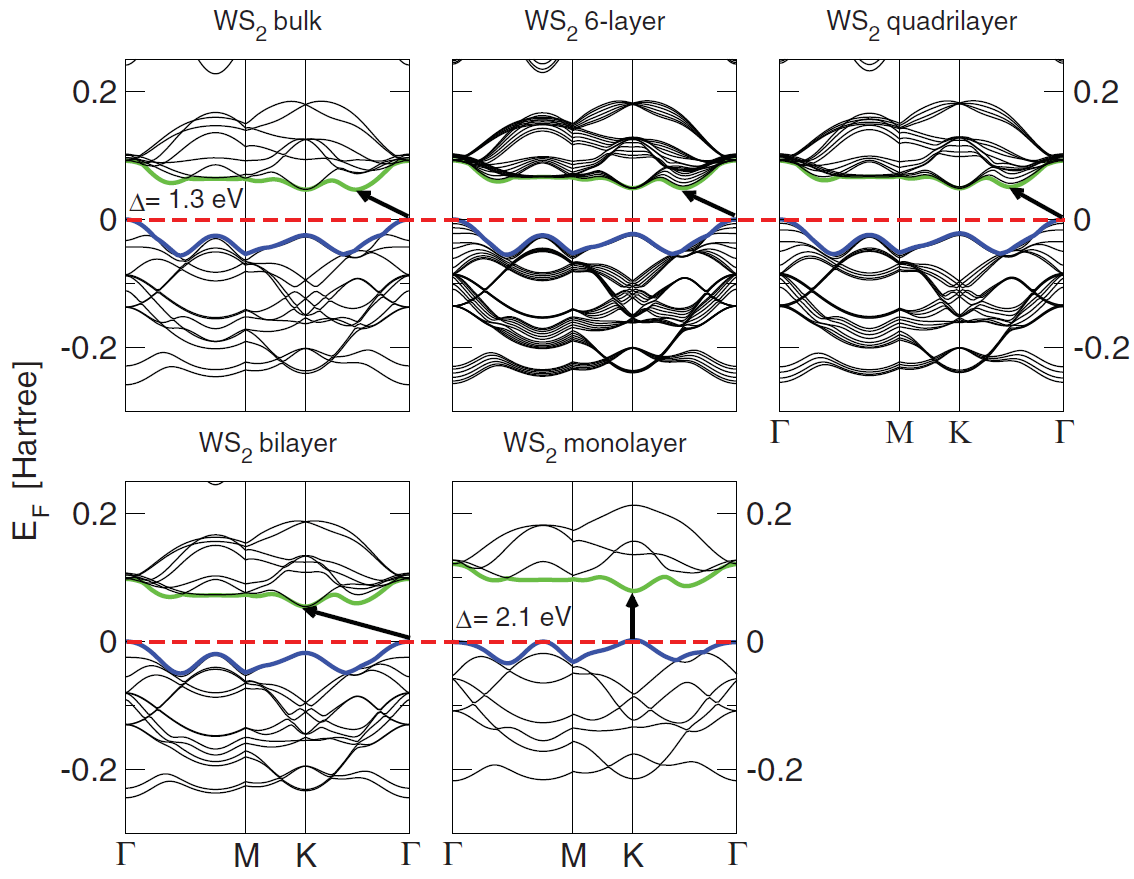
\includegraphics[scale=0.4]{WS2BandStructureSimulation.png}
	\caption{Band structures of bulk $WS_2$, its monolayer, as well as, polylayers calculated from the density functional theory (DFT) simulation. The horizontal dashed lines indicate the Fermi level. The arrows indicate the fundamental band gap (direct or indirect) for a given system. The top of valence band (blue) and bottom of conduction band (green) are highlighted. Adopted from Ref. \cite{WS2BandStructureSimulation}}
	\label{fig:WS2BandStructureSimulation}
	\end{center}
	\end{figure}
	
	Like $WS_2$ other Mo and W based TMDC undergo similar transitions as seen in Table \ref{tab:MoWBandgapsComparison}. In all cases the smaller indirect bandgap changes to greater direct bandgap with monolayer bandgap ranging from 1.1 eV to about 2.1 eV. Moreover the VBM at K points exhibits the orbit-spin band splitting at the K point of about 400 meV. This direct bandgap leads to presence of A and B excitons generated by transition between CBM and two VBMs at the K point. The conduction band as well as the valence band are dominated by the d-electron orbitals of the transition metal atoms and at the VBM and CBM they hybridize with the p-electron orbitals of the chalcogenide atoms. Because the hybridization happens mostly at the $\Gamma$ point and the chalcogenide atoms are at the surface of the TMDC layer it leads to strong interactions between the layers. This leads to significant change in the band structure at the $\Gamma$ and rise of the indirect bandgap as a result of increased number of layers. On the other hand at the $K$ point the d-orbitals of the transition metals remain mostly unaffected due to them being positioned in the middle of the layer \cite{WS2BandStructureSimulation} \cite{EmergingPhotoluminescenceInMonolayerMoS2}
	 
	 \begin{table}[h]
	 \caption{Mo and W based TMDC bandgaps comparison. Adopted from \cite{ElectronicsAndOptoelectronicsOfTwo-dimensionalTransitionMetalDichalcogenides}}
	 \label{tab:MoWBandgapsComparison}
	 \end{table}
	 
	 \begin{center}
	 \begin{tabular}{c|l|l|l}
	 
	 M$\backslash$X & $-S_2$ 			& $-Se_2$ 			& $-Te_2$			\\ \hline
	 Mo 			& Semiconducting	& Semiconducting	& Semiconducting	\\ 
	 				& 1L:1.8 eV			& 1L: 1.5 eV		& 1L: 1.1 eV		\\
	 				& Bulk: 1.2 eV		& Bulk: 1.1 eV		& Bulk: 1.0 eV		\\ \hline
	 W 				& Semiconducting	& Semiconducting	& Semiconducting	\\
	 				& 1L:2.1 eV			& 1L: 1.7 eV		& 1L: 1.1 eV		\\
	 				& Bulk: 1.4 eV		& Bulk: 1.2 eV		& 					\\
	 
	 \end{tabular}
	 \end{center}
	
	
	\subsection{Optical properties}
	\label{subsec:Optical properties}

	TMDCs exhibit a wide array of opto-electronic effects due to their strong light-matter effects. These effects are mostly caused by the abundant presence of excitons, bi-excitons, trions or bound excitons. As a result the change in layer thickness from bulk to monolayer alters the photoluminescence, photoconductivity and absorption in the visible to infrared range.
		
	The primary and most common quasi-particle that forms in such system is an exciton, which is a pair of a negatively charged electron and a positively charged hole bound together by Coulomb forces to form a structure similar to that of hydrogen atom. Such pair is electrically neutral and is of size exceeding size of single cell which makes it a Wannier–Mott exciton. The recombination of these excitons results in a photon emission which can be easily observed during photoluminescence characterisation. On top of excitons other quasi-particles such as trions, bi-excitons or bound excitons can be found. A trion is a group of 2 electrons and a hole or 2 holes and an electron, or otherwise described as a charged exciton. The exact nature of the trion depends usually on the type of intrinsic doping of the TMDC. A bi-exciton is a pair of excitons which is usually only observed in quantum dot systems but can be also seen in excitonically dense systems such as TMDCs. A bound exciton is similar to the free exciton but is trapped by a defect. In a typical photoluminescence spectrum several peaks can be observed depending on specific type of TMDC characterised. In $WS_2$ monolayer for instance as seen in Figure. \ref{fig:WS2TypicalPLSpectra} the strongest peak (often labelled as an A peak) at about 1.97 eV is caused by the direct transition of single-photon generated exciton. Slightly redshifted by about 30 meV from the A peak a generally weaker peak caused by the trion recombination can be found. At higher energies another peak can be observed due to the presence of bi-excitons. At around the 1.3 eV a much weaker peak (I) can be seen caused by the indirect transition. Additionally a B peak can be observed blueshifted from the A peak which is caused by valley splitting as discussed in chapter \ref{subsec:Electronic properties}. As seen in Figure \ref{fig:WS2TypicalPLSpectra} as the number of layers increases the main A peak becomes dramatically weaker due to lack of direct transition and redshifted following the pattern discussed in chapter \ref{subsec:Electronic properties}. At the same time the I peak becomes relatively stronger and eventually dominates the bulk material.
		
\begin{figure}[h]
	\begin{center}
		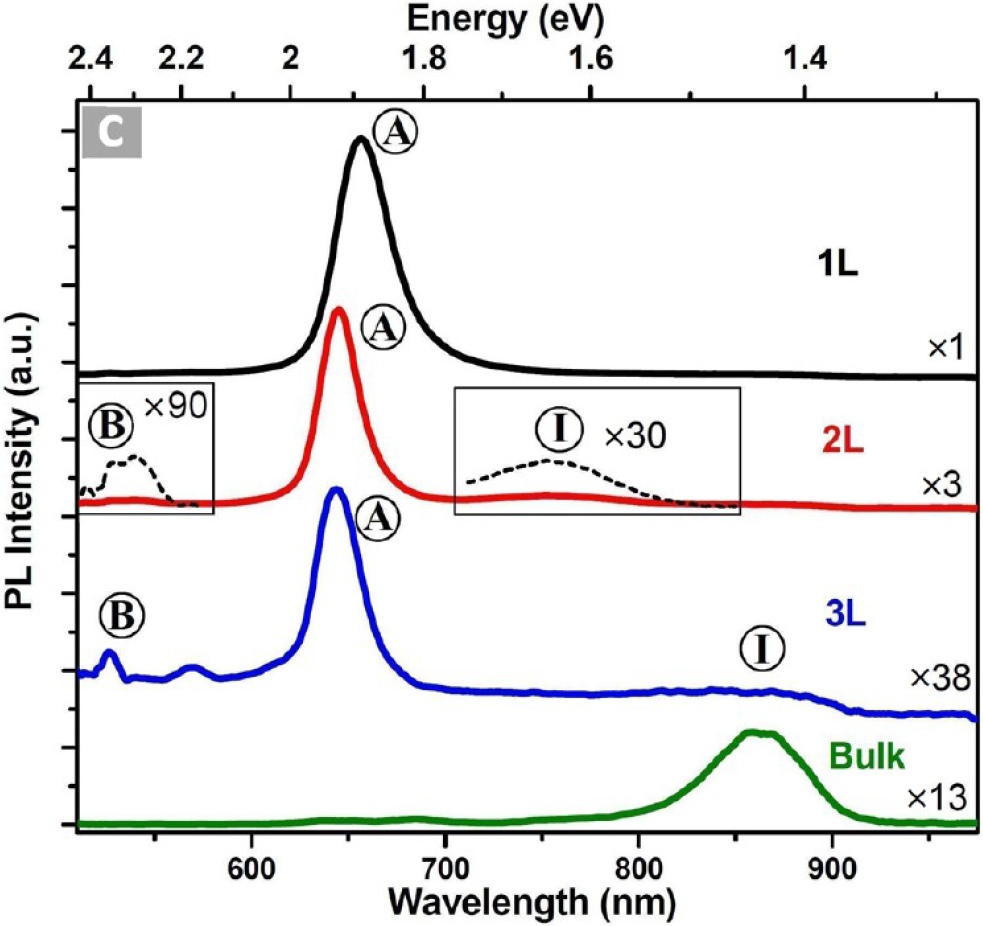
\includegraphics[scale=0.3]{WS2TypicalPLSpectra.png}
		\caption{Typical PL spectrum of $WS_2$}
		\label{fig:WS2TypicalPLSpectra}
	\end{center}
\end{figure}
		
	Similarly the photoconductivity of the TMDCs is strongly reliant on the number of layers and incident photon energy. The $MoS_2$ for instance shows 3 times stronger photoconductivity in monolayer around 1.8 eV, where the direct transition is located, than in 2L $MoS_@$ around 1.6 eV. Additionally the photoconductivity appears to increase in steps with relation to the photon energy following the direct and indirect transitions. \cite{ElectronicsAndOptoelectronicsOfTwo-dimensionalTransitionMetalDichalcogenides}.
		
	The sunlight absorption in TMDCs has been shown to be significantly more intense than in commonly used solar cell materials, at about 5-10$\%$ which is an order of magnitude greater compared to similar thickness of Si or GaAs. It is also stronger compared to 2-3$\%$ of sunlight absorption of graphene. As a result a excitonic solar cell based on $MoS_2/WS_2$ bilayer shows about 1$\%$ power efficiency, about 3 times greater than that of typical ultrathin solar cells \cite{ExtraordinarySunlightAbsorptionAndOneNanometerThickPhotovoltaicsUsingTwo-DimensionalMonolayerMaterials}.
	
	During standard single photon excitation photoluminescence studies the excitons generated can be called "bright" since they appear in PL spectrum. The reason we can observe them easily is because the spin between an electron and a hole is conserved, and thus allowing for photon emission. However another combination is possible, called dark exciton, where both electron and the hole have the same spin. Because of that they cannot recombine by emitting a photon and therefore remain absent from the PL spectrum. Even though they exist much longer than their bright counterparts their presence is of course also more difficult to observe. One way to observe them is to use two photon excitation. Due to two photon selection rule the single photon excitation can be excluded and the dark excitonic states can be observed. In $WS_2$ the dark excitons result in two peaks at 2.28 eV and 2.48 eV. \cite{Ye2014}
	
	Defect engineering allows to tune the number of charge carriers. In $MoS_2$ or $WS_2$ the sulfur vacancies lead to increased number of electrons in the material. Because of that by increasing the number of defects in those materials the level of n-doping can be changed. An easy way to observe the presence of those defects and subsequent quenching of them is to expose the material to varying amounts of oxygen, nitrogen or water. Those species attract the electrons locally and therefore the electron population in the material decreases. This in turn leads to smaller trion population since trions require an extra electron to form. This then can be observed in PL as a more narrow direct peak, with especially smaller redshifted shoulder. The effect can also be of course reversed by decreasing the amount of oxygen, nitrogen or water in the environment since those exist in already in ambient conditions \cite{Currie2015}.
	
	In order to introduce and control the amount of vacancies in the TMDC different method have to be explored. One of the ways of achieving that in already grown material is the use of oxygen plasma. It has been shown that the number of defects can be controlled by limiting the plasma exposure. During the process the oxygen also chemically bonds to the MoS2 at the defect sites and therefore partially negates the effect of defects on the optical properties. The PL can also be seen to increase in intensity with increasing number of defects with oxygen adsorped due to the increased yield of bound excitons localised at these defects \cite{Nan2014}.
	
	Similar effect has been shown using the 2,3,5,6-tetrafluoro-7,7,8,8-tetracyanoquinodimethane ($F_4TCNQ$), 7,7,8,8-tetracyanoquinodimethane ($TCNQ$) and (nicotinamide adenine dinucleotide) $NADH$ for chemical doping. Both $F_4TCNQ$ and $TCNQ$ are p-type dopants while $NADH$ is a n-type dopant. By exposing the surface of $MoS_2$ to these compounds the change in PL intensity and FWHM have been observed. Similar to doping with $O_2$, $N_2$ or $H_2O$, all of which are p-type dopants, the intensity of PL has increased in presence of $F_4TCNQ$ and $TCNQ$. The effect has been similarly ascribed to lowering the number of defects and therefore the lowering the trion population and subsequently increasing the exciton population increasing the yield. The opposite observation has been made with use of $NADH$ with PL intensity decreasing. Similarly the increase in trion population with lower PL yield is ascribed to the lower PL intensity. \cite{Mouri2013}
	
	It has also been show that alloying can be used to fine tune the PL by varying the concentration of alloying material. In monolayer $Mo_{1-x}W_xS_2$ the PL peak position initially decreases from 1.575 eV (PL peak position of pure $MoS_2$) to 1.56 eV at x=0.21 and then increase up to 1.65 eV (PL peak position of $WSe_2$) at x = 1. This effect could be attributed to the linearity of VB and non-linearity of CB with regards to change in W composition. The PL position can therefore be engineered on a monotonic range from 1.56 eV to 1.65 eV. In bilayer $Mo_{1-x}W_xS_2$ alloy the position of both direct and indirect transition PL peaks increases monotonically from about 1.49 eV and 1.53 eV for pure MoSe2 to 1.56 eV and 1.62 eV for pure $WSe_2$ as the W amount is increased. This opens another relatively easy way of engineering PL position \cite{Zhang2014}.
	
	Another effect that has been demonstrated that allows for certain degree of control of PL in TMDCs is relation between the helicity of incident light and valley population valley population. It has been shown that by exciting the monolayer $MoS_2$ with right-polarised light the resulting excitons will fill primarily the VB at K point. Similarly by exciting the $MoS_2$ with left-polarised light the excitons will fill the VB at K' point. After recombination the resulting photons will exhibit the same circular polarity as the photons that excited the electrons in the first place. \cite{Mak2012}\cite{Mak2012a}
	
	The temperature effect on TMDCs has also been investigated. In $WSe_2$ monolayer it has been shown that as the temperature of the sample increases from room temperature to about 400K the position of the direct transition PL peak redshifts from about 1.65 eV to about 1.58 eV. When the temperature is decreased from room temperature to about 5K the same peak blueshifts to about 1.7 eV. Between 100K and 50K as well 20K and 5K the position of the PL peak does not change. Additionally around 120K another peak appears and as the temperature is lowered it also blueshifts although less than the RT peak. The peak only present at RT is attributed to free excitons whereas the peak appearing at 120K is ascribed to bound excitons. As bound exciton peak appears its intensity increasese with lower temperature while the intensity of the free exiton peak decreases. This indicates that the population of free excitons decreases while the population of the bound excitons increases with decreasing temperature \cite{PhotoluminescencePropertiesAndExcitonDynamicsInMonolayerWSe2}
	
	There has been many reports on the spatial distribution of PL in the TMDCs. One of the observed patterns in $WS_2$ and $MoS_2$ has been that of much stronger PL intensity at the edges of the flakes. That effect has been primarily observed in small flakes of about 5 $\mu m$ \cite{ExtraordinaryRoomTemperaturePhotoluminescenceInTriangularWS2Monolayers}. X

Direct band-to-band transitions in two-dimensional system are characterized by a step-function-like spectrum originated from the energy-independent joint-density-of-states and transition matrix elements near parabolic band edges \cite{Haug1994} (dashed blue line in Figure \ref{fig:TMDCAbsorption}). However, TMDCs  are dominated by excitonic effects as exemplified by experimental absorption spectrum with sharp resonance features \cite{EmergingPhotoluminescenceInMonolayerMoS2} (solid green line in Figure \ref{fig:TMDCAbsorption}). These excitonic effects are enabled by the very large exciton binding energies $E_B$ (0.5–1 eV, corresponding to an exciton Bohr radius $a_B \approx 1 nm$) at room temperature which has been predicted theoretically and measured experimentally using optical spectroscopy and scanning tunnelling spectroscopy. Some discrepancies in the estimated value are still present but overall theory and experiment broadly agree. 
In addition to excitons, higher-order excitonic quasiparticles have also been observed in 2D TMDs (Figure \ref{fig:TMDCQuasiparticles}). Trions, which are bound states of two electrons and one hole, or two holes and one electron, have been observed in intrinsically doped monolayer TMDCs \cite{Mak2012}\cite{Ross2013}. Bi-excitons (bound states of two excitons) have been reported in monolayer TMDCs under pulsed optical excitations \cite{doi:10.1021/nn5059908}\cite{You2015} and the quinton (the five-particle negatively charged biexciton) \cite{Barbone2018}.
 
The existence of trions at room temperature and higher-order excitonic quasiparticles  in general, may open up many applications for room-temperature electrical transport of absorbed light energy, and creation of high-temperature and high-density quantum coherent states of excitons.
The very high excitonic effects also generate a significant transfer of oscillator strengths from the band-to-band transitions to the fundamental 1s exciton state \cite{Haug1994}. The ratio between the oscillator strength of the 1s ($f_{1s}$) and the band-to-band ($f_0$) transitions has been estimated  from the ratio of the width $\Delta$ of the 1s state (~10 meV) and exciton binding energy $E_B$ (~0.5 eV), the exciton reduced mass $\mu$ and total mass M (\cite{Feldmann1988}\cite{Haug1989}) using the following equation:

\begin{equation}
f_{1s}/f_0 \approx 24({\mu}/M)(E_B/{\Delta}) \approx 100
\end{equation} 
 
This provides a value of 100 which is a large exciton oscillator strength which gives rise to a strong light absorption. Indeed, peak absorbance as large as $A_0 \approx 0.1–0.3$ are observed at the exciton 1s state \cite{AtomicallyThinMoS2ANewDirect-GapSemiconductor}\cite{Mak2012}. Furthermore, the strong excitonic effects lead to a  short radiative lifetime $1/{\Gamma}_{1s}$ (\cite{Feldmann1988}\cite{Haug1989}). This can be estimated using the following equation: $1/{\Gamma}_{1s} = (f_0/f_{1s})(1/{\Gamma}_{r0})$
This value is $\approx 10–100 ps$ at low temperature considering a typical band-to-band radiative lifetime to be $1/{\Gamma}_{r0} \approx 1–10 ns$. Atomically pristine materials could potentially present even shorter radiative lifetime. 


\begin{figure}[!h]
	\begin{center}
		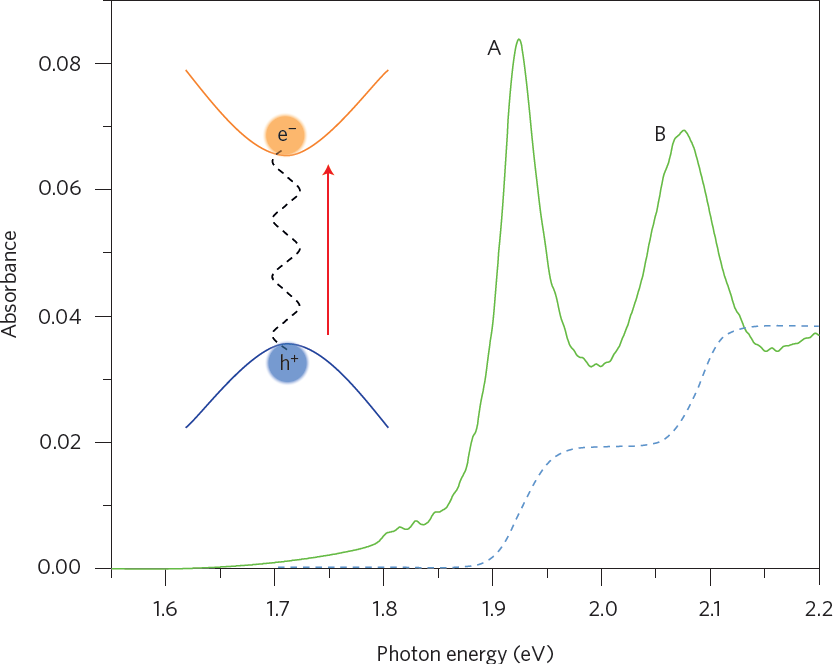
\includegraphics[scale=0.45]{TMDCAbsorption.png}
		\caption{Absorption spectrum of monolayer MoS2 at 10 K (solid green line). A and B are exciton resonances corresponding to transitions from the two spin-split valence bands to the conduction bands. The blue dashed line shows the absorbance (arbitrary units) if excitonic effects were absent. The inset illustrates the Coulomb attraction between an optically generated electron–hole pair, forming a bound exciton. Reproduced from \cite{Mak2016}}
		\label{fig:TMDCAbsorption}
	\end{center}
\end{figure}

\begin{figure}[!h]
	\begin{center}
		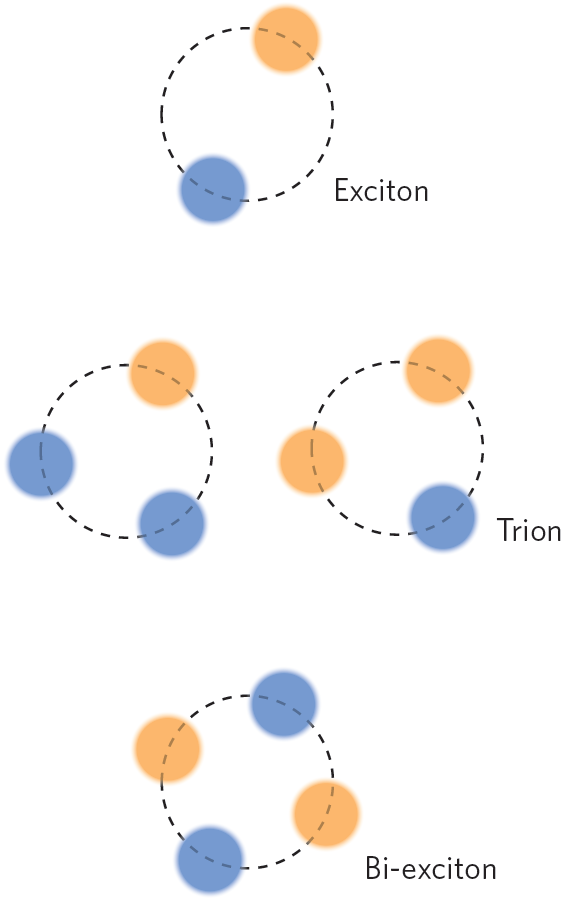
\includegraphics[scale=0.35]{TMDCQuasiparticles.png}
		\caption{Illustration of exciton and higher-order excitonic complexes: a two-particle charge-neutral exciton, a three-particle charged exciton (trion) and a fourparticle bi-exciton. Reproduced from \cite{Mak2016}}
		\label{fig:TMDCQuasiparticles}
	\end{center}
\end{figure}


\subsection{Optoelectronics applications} 

Here I summarize the main developments in optoelectronic devices based on 2D TMDs, in particular photodetectors, excitonic light-emitting devices (LEDs) and optical generation of spin–valley currents. 

\subsubsection{Photodetectors}

TMDC photodetectors are still at the early stages of development and they have been used and demonstrated in the same operational wavelengths as silicon. 2D TMDCs, however present intrinsic advantages over silicon  which are the mechanical flexibility and electronically highly tunability.
2D TMDC photodetectors operate mostly on the basis of the photovoltaic effect and exhibit low dark currents and high responsivity while the operation speed remain limited. Significant improvements should be possible given the short exciton lifetimes in these materials (~10–100 ps)\cite{Massicotte2015}\cite{Korn2011}\cite{Wang2012}. The operation modes of photodetection based on the photovoltaic effect can be divided \cite{Sze2002} into two categories: photoconduction, and photocurrent. Photoconduction is based on photoexcited carriers which increase the device's conductance, while the photocurrent, in which photoexcited carriers are converted into current with the help of a built-in electric field originated from a symmetry-lowering element such as a junction (p-n junction).
Experimental demonstration of photodetectors are based on both in-plane and out-of-plane structures of 2D TMDCs (Figure \ref{fig:PhotodetectorDiagram} and Figure \ref{fig:PhotoconductorDiagram}). In-plane devices allows to control the material's properties through electrostatic gating which offers a better accuracy than the out-of-plane devices. However the latter can support a much higher bias field (up to ~1 V $nm^{–1}$) which can enable a more efficient exciton dissociation. Indeed exciton dissociation in TMDCs is key due to the very high binding energy and in case of tunnelling ionization of excitons the process becomes inefficient when a bias electric field is small compared with $E_B/(ea_B) \approx 0.2 V nm^{–1}$ (a very large field indeed)\cite{Haug1994} while excitons dissociation is effectively achieved by electric fields (either built-in or externally applied).

There has been many successful attempts in making photodetectors based on photoconductivity and utilising TMDCs as an active material. Monolayer $MoS_2$ has been used for a transistor achieving responsivity of 880 $AW^{-1}$ with a bandwidth of $~0.1 Hz$ (Figure \ref{fig:PhotodetectorDiagram}) \cite{Lopez-Sanchez2013}. A much better bandwidth ($>10 kHz$) and therefore a faster device has been achieved, but with a smaller responsivity of $~1 AW^{-1}$ \cite{Tsai2013}. The large photogain is associated with the trapped carrier at the interface states \cite{Katz2001}. The devices conductivity tends to be modified primarily by the doping as well as trapped states \cite{Tsai2013} \cite{Furchi2014}.

Similarly devices based on photocurrent for photodetection hase been achieved. These can be made by creating a junction both out of plane \cite{Withers2015}\cite{Cheng2014} as well as in plane \cite{Ross2014}\cite{Fontana2013}. $WSe_2$ has been used to make an in plane p-n junction with a depletion region of up to 500 nm and a resulting field of 0.02 $V nm^{-1}$.  In such a device a responsivity of $~1 mAW^{-1}$ and $~200 mAW^{-1}$ was demonstrated under zero bias and a forward bias respectively \cite{Baugher2014}. Due to large diffusion length of excitons it is difficult to achieve both wide depletion area as well as a strong built in field to dissociate strongly bound excitons. On the other hand the out of plane heterojunctions made out of one n-type (e.g. $MoS_2$) and one p-type (e.g. $WSe_2$) layers can rectify these issues. Such built device can achieve very high in built electric fields of $~1 V nm^{-1}$ and a zero bias responsivity of $~0.1 A W^{-1}$ \cite{Cheng2014}\cite{Lee2014}. 

\begin{figure}[!h]
	\begin{center}
		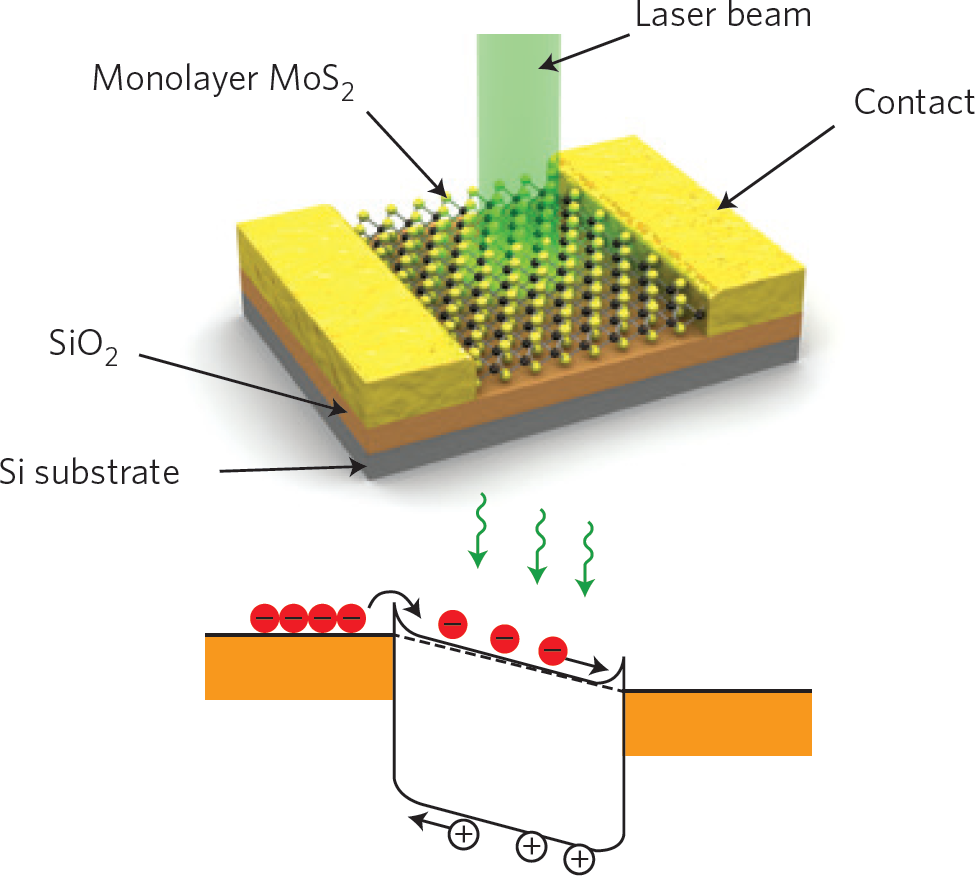
\includegraphics[scale=0.35]{PhotodetectorDiagram.png}
		\caption{Top: Schematic of monolayer MoS2 lateral photoconductor. Bottom: Band diagram of
the monolayer $MoS_2$ photodetector taking into consideration small Schottky barriers at the contacts (on state of the device). Reproduced from \cite{Mak2016}}
		\label{fig:PhotodetectorDiagram}
	\end{center}
\end{figure}

\begin{figure}[!h]
	\begin{center}
		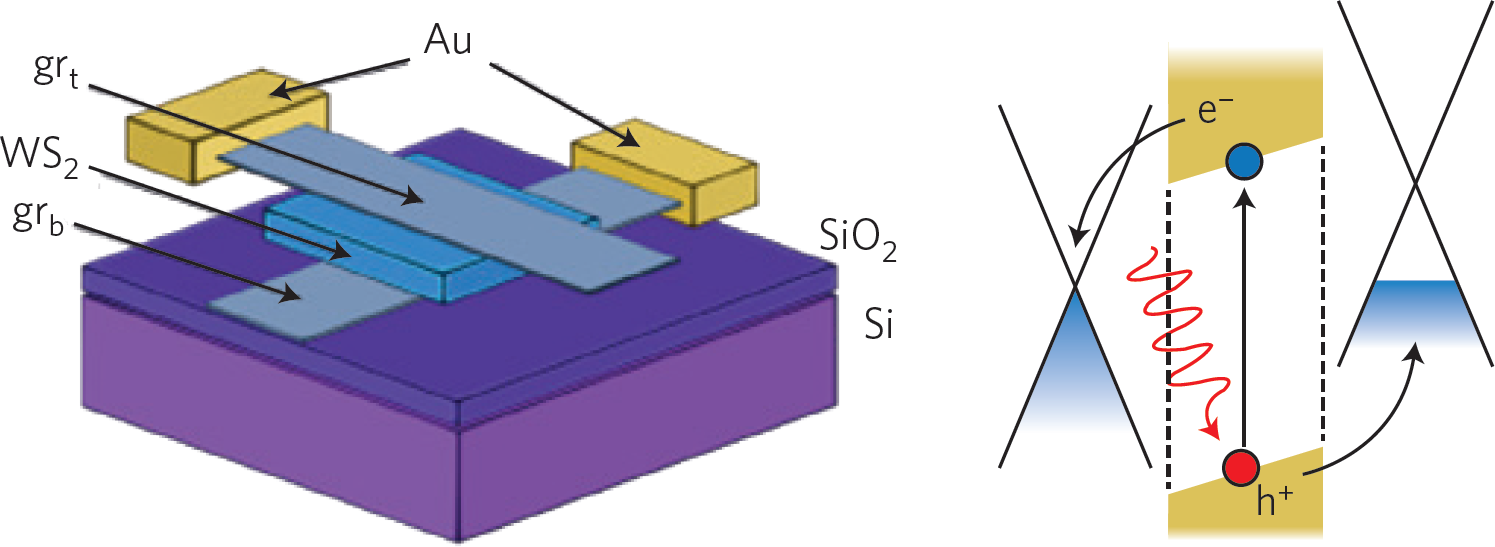
\includegraphics[scale=0.25]{PhotoconductorDiagram.png}
		\caption{Left: Fewlayer $WS_2$ vertical photoconductor with graphene top ($g_{rt}$) and back ($g_{rb}$) electrodes. Right: Schematic band diagram for a graphene/$WS_2$/graphene heterostructure with a built-in electric field to separate the generated electron–hole pair. Reproduced from \cite{Mak2016}}
		\label{fig:PhotoconductorDiagram}
	\end{center}
\end{figure}

\newpage
\begin{table}[!ht]
	\label{tab:GrapheneTMDCPhotodectorsComparison}
	\caption{Comparison of performances of graphene and 2D TMD photodetectors}
\end{table}

\begin{tiny}
\begin{center}
\begin{tabular}{l|llll}

									& Device type		& Responsivity				& Bandwidth			& Quantum efficiency	\\\hline
									& Photoconduction	& 							&					&						\\	
Near-infrared to visible gap		& In-plane			& $~1-10^3 AW^{-1}$			& 0.1 Hz to $>10$ kHz & ~50\% (E) 			\\
Strong exciton binding				& Out-of-plane		& $~0.1 AW^{-1}$			& $\leq$200 GHz 	& 						\\
Mainly based on photovoltaic effect & Heterojunction 	& 							& 					&						\\
Low dark current					& In-plane			& $1 mAW^{-1}$ (zero bias)	& - 				& ~2\% (I) (zero bias) 	\\
									& Out-of-plane		& $~100 mAW^{-1}$ (zero bias)& -				& ~10-30\% (E) (zero bias) \\\hline
\multicolumn{5}{l}{I and E are internal and external quantum efficiencies, respectively. LT, low temperature; RT, room temperature.}

\end{tabular}
\end{center}
\end{tiny}


	
\section{Phonon dispersion}
	
	The vibrational and phononic characteristics of TMDCs have been investigated at length by both theoretical simulations as well as experimental studies. The $2H-MX_2$ crystal structure of the TMDCs belongs to $D_{6h}^4$ point group and there are 18 lattice dynamical modes at the $\Gamma$ point. Phonons belonging to these modes can be represented as Eq. \ref{eq:PhononDispersionRepresentation} \cite{LatticeDynamicsInMono-AndFew-LayerSheetsOfWS2AndWSe2}: 
	
\begin{equation}
	{\Gamma} = A_{1g} + 2A_{2u} + B_{1u} + 2B_{2g} + E_{1g} + 2E_{1u} + E_{2u} + 2E_{2g}
	\label{eq:PhononDispersionRepresentation} 
\end{equation}
	
	In TMDCs 4 active Raman modes can be observed $E_{1g}, E^1_{2g}, E^2_{2g}, A_{1g}$. These can be seen in Figure \ref{fig:4ActiveRamanModes}. The $E^2_{2g}$ is a shear mode that involves 2 layers vibrating against each other. The $E_{1g}$ is an in-plane vibration of chalcogen atoms but is forbidden in the back-scattering configuration. For monolayers therefore it leaves primarily the $E^1_{2g}$ which is an in-plane mode involving vibration of both metal and chalcogen atoms as well as $A_{1g}$ which is an out-of-plane mode involving only chalcogen atoms. 
	
\begin{figure}[h]
	\begin{center}
		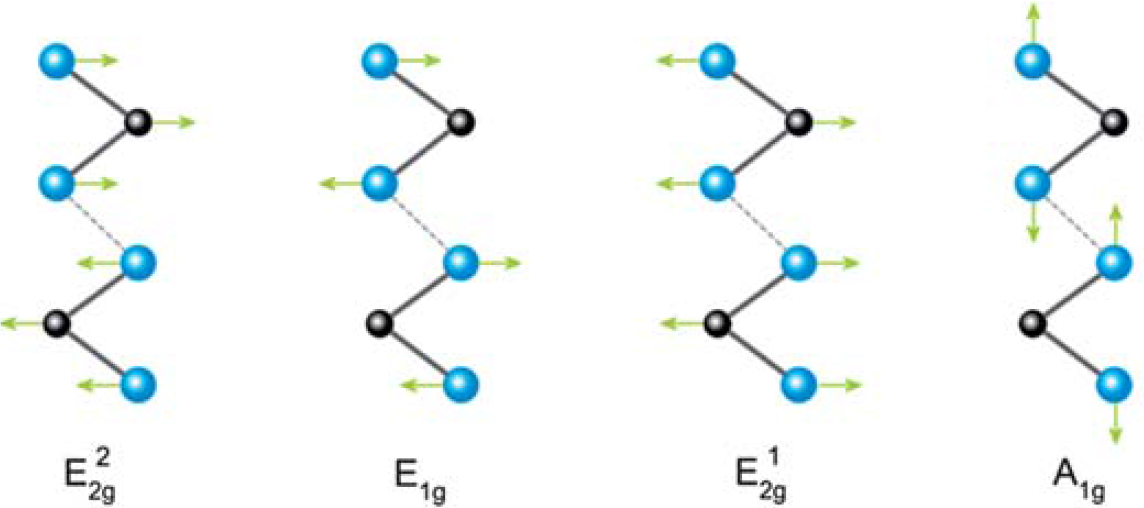
\includegraphics[scale=0.4]{RamanActiveModes.png}
		\caption{4 active Raman modes in TMDCs. Metal atoms and chalcogen atoms are black and blue respectively. Adopted from \cite{LatticeDynamicsInMono-AndFew-LayerSheetsOfWS2AndWSe2}}
		\label{fig:4ActiveRamanModes}
	\end{center}
\end{figure}
	
	These two peaks tend to dominate the spectrum of any TMDCs, whether monolayer or few-layer or bulk. The shear mode $E^2_{2g}$ appears at low Raman shift frequencies and is therefore difficult to observe but can be used to differentiate monolayer from few-layer material. Since $E^1_{2g}$ is an in-plane mode it tends to be unaffected by the number of layers due to weak van der Vaals forces between the layers but can be seen to be slightly redshifted as the number of layers increases. As seen in Figure \ref{fig:TypicalRamanSpectrumWS2} the $E^1_{2g}$ peak at about 352 $cm^{-1}$ is overlapping with another stronger peak, a 2LA(M) peak at 350 $cm^{-1}$ which is a longitudinal acoustic mode caused by in-plane collective oscillations of W and S atoms. The second strongest peak at around 416 $cm^{-1}$ is an $A_{1g}$ peak, caused by out of plane vibrations. Because of that it is much more sensitive to the number of layers and is seen to become blueshifted as the number of layers increases. This has been attributed to the restorative forces as well as increase in dielectric screening of the Coulomb forces. Combining both of these shifts in frequency with the changing number of layers the difference between these two peak position can be used to identify the number of layers in TMDCs as seen in Figure \ref{fig:LayerNumberIdentificationRamanShiftWS2}
	
\begin{figure}[h]
	\begin{center}
		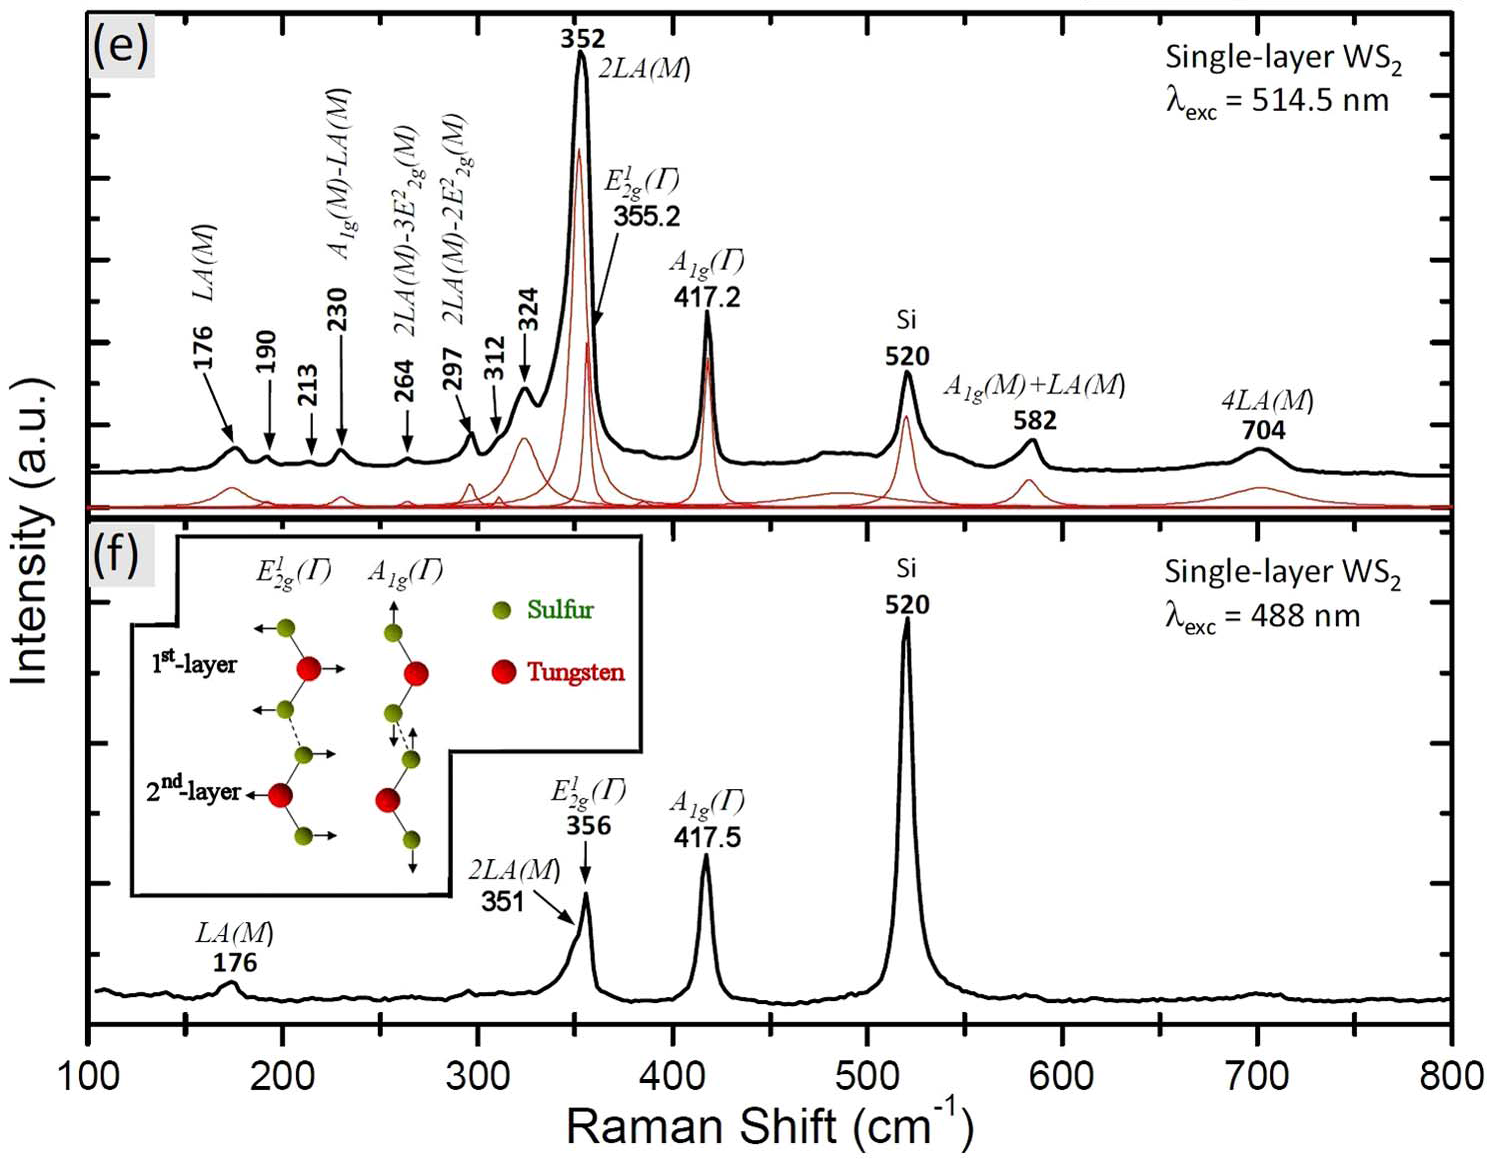
\includegraphics[scale=0.3]{RamanPeaksIdentification.png}
		\caption{Typical Raman spectrum of $WS_2$. Adopted from \cite{Berkdemir2013}.}
		\label{fig:TypicalRamanSpectrumWS2}
	\end{center}
\end{figure}
	
\begin{figure}
	\begin{center}
		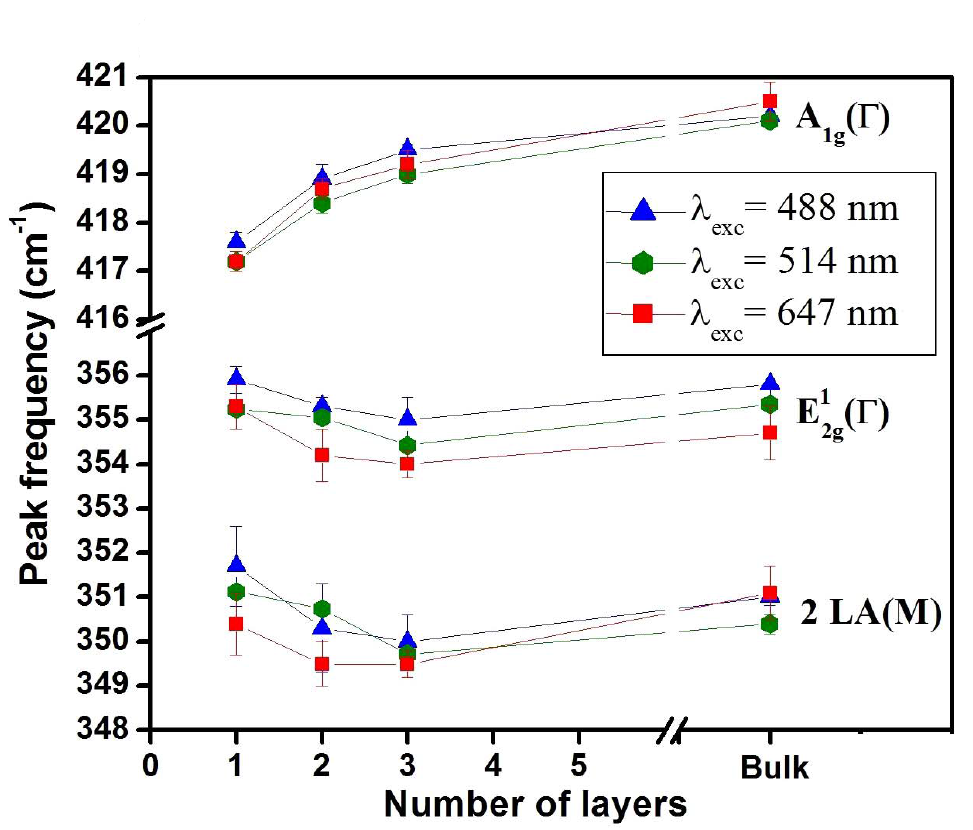
\includegraphics[scale=0.3]{NumberLayerIdentificationRaman.png}
		\caption{Identification of number of layers by the difference in position of $A_{1g}$ and $E^1_{2g}$ peaks. Adopted from \cite{Berkdemir2013}.}
		\label{fig:LayerNumberIdentificationRamanShiftWS2}
	\end{center}
\end{figure}

Similarly in $MoS_2$ the $E^1_{2g}$ and $A_{1g}$ peaks can be observed easily using Raman spectroscopy. The position of the monolayer $E^1_{2g}$ and $A_{1g}$ peaks are found to be about $385 cm^{-1}4 and 403 cm^{-1}$ respectively. Unlike the $WS_2$ and especially in monolayer form the $E^1_{2g}$ does not overlap with the 2LA peak which helps greatly with resolving and peak fitting individual peaks. Similarly to the $WS_2$ the peak position of those two peaks changes with the number of layers in a same manner. As the number of layers increases from monolayer to bulk the $E^1_{2g}$ shifts a small amount to the red being largely unaffected since that vibrational mode exists in plane and is therefore not influenced by the layer above or below. The $A_{1g}$ on the other hand, similarly to the $WS_2$ $A_{1g}$ peak blueshifts by relatively larger amount due to out of plane vibrations which are affected by the number of layers. The separation between those two peaks can be used therefore as an indicator of the number of layers similarly to the $WS_2$. 

\begin{figure}[h]
	\begin{center}
		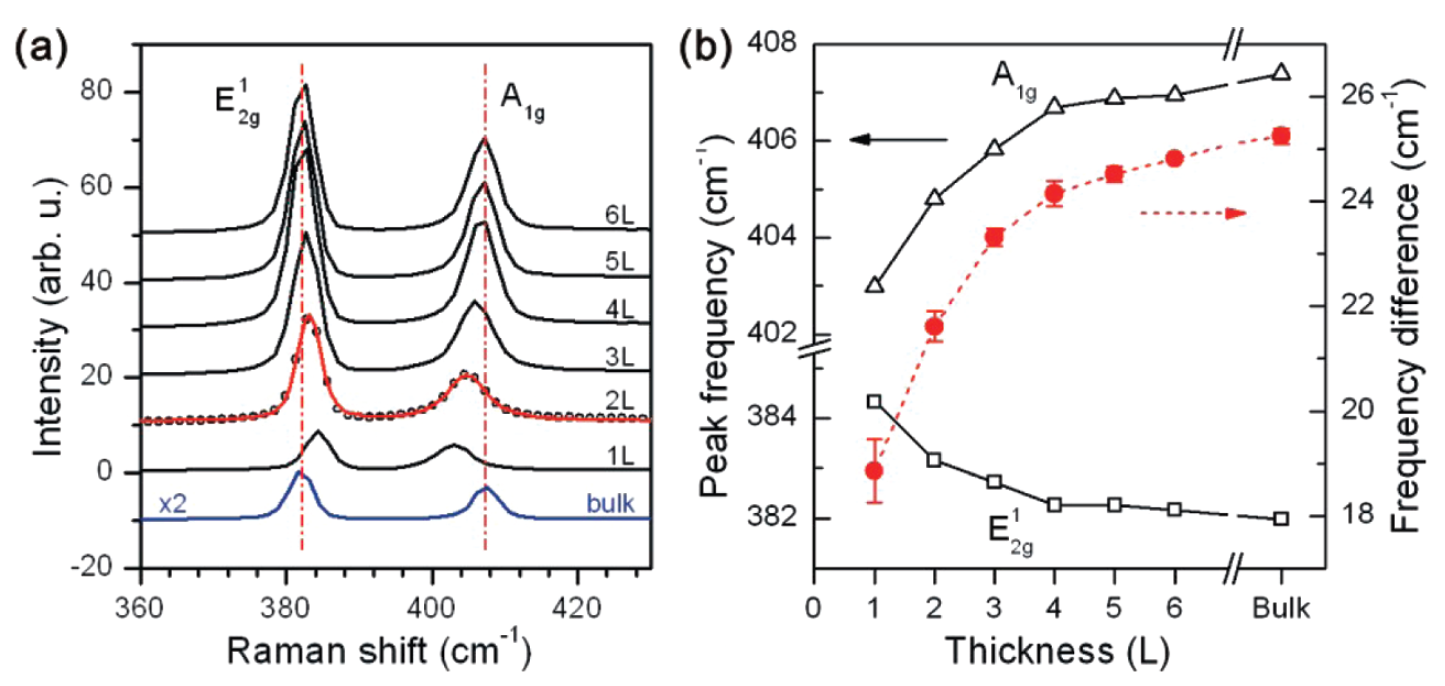
\includegraphics[scale=0.3]{NumberLayerIdentificationRamanMoS2.png}
		\caption{(a) Raman spectra of thin (nL) and bulk $MoS_2$ films. The solid line for the 2L spectrum is a double Voigt fit through data (circles for 2L, solid lines for the rest). (b) Frequencies of $E^1_{2g}$ and $A_{1g}$ Raman modes (left vertical axis) and their difference (right vertical axis) as a function of layer thickness. Adopted from \cite{Lee2010}.}
		\label{fig:NumberLayerIdentificationRamanMoS2}
	\end{center}
\end{figure}

\section{Conclusions}

In this chapter we have presented and discuss the electronic and vibrational properties on group VI TMDs with a specific focus on $WS_2$ and $MoS_2$. We have summarized the current state of the art which involves experimental and simulation studies. In conclusion mono- and few layer TMDCs have become an important class of materials to study in recent years. Despite their knowledge and usage in bulk forms for many more years their atomically thin form remained largely unexplored. Their particularly interesting properties arise most strikingly when the number of layers is very small. The sulphides and selenides of group VI transition metals  (Mo and W) exhibit an indirect to direct bandgap placed in visible to infrared range, high electronic mobilities of ~$10^3$ $cm^2 V^{-1} s^{-1}$, FET switch ratio of $>10^7$ and strain rates up to 20{\%}. Those materials provide therefore a great potential for many applications in electronic and optoelectronic devices for light detection, emission and harvesting. One of the limiting factors in future development of material synthesis and devices is understanding of the TMDCs properties and ability to characterise them easily.
\chapter{Methodology}

\section{Introduction}

In order to characterise the synthesised materials and acquire information about the chemistry, crystallinity, morphology as well as its optical and electrical properties a suite of state of the art techniques has to be utilised. An overview of those techniques has been provided in theory and experimental setup.

\section{Raman spectroscopy}

Raman spectroscopy is one of the most useful and versatile characterisation techniques for 2D TMDCs due to its non destructive and ease of use. The lack of need to extensively prepare the sample like in some other techniques allows for relatively fast measurements of a large number of samples. Additionally the lack of transfer required results in minimal changes to to the material itself as well allows for easier tracking of specific areas of the sample across different techniques. Raman spectroscopy can be used to measure as grown by CVD samples on $Si/SiO_2$ substrate or any other solid substrate as well as liquid solution samples produced by liquid exfoliation.

The Raman spectroscopy can be used to extract information about the chemistry of the material as well as the crystal structure, the number of layers of 2D TMDCs or the strain within the layers. 

When a material is irradiated with light the photons generally scatter at different angle but same wavelength. However certain small part of the incident photons (about 1 in 10 million) is scattered at different wavelength than the incident one. This is known as the Raman effect and the photons that are scattered at wavelengths greater than the incident ones are due to Stokes scattering, while the ones emitted at wavelengths smaller than the incident one are due to anti-Stokes scattering. In the Stokes scattering phenomena the phonon is emitted while during the anti-Stokes scattering the phonon is absorbed as seen in Figure \ref{fig:MethodologyRamanEnergyLevels}. In order for the Raman effect to take place a transition between two resonant states must occur. The probability of transition from lower to higher energy state depends on the population of the states. In a thermodynamically stable system the lower energy states are more occupied than the higher energy and therefore the transition from lower to higher is more likely to occur (Stokes scattering). The spectrum of photons scattered as a result of Raman scattering forms what is known as Raman spectrum, where the number of photons scattered is plotted against the photon frequency difference between the incident and the scattered photons. The spectrum is symmetrical around the spectrum origin in regards to the frequency but not in terms of intensity. Because of that only the Stokes part is generally used as a Raman spectrum.

\begin{figure}[!h]
	\begin{center}
		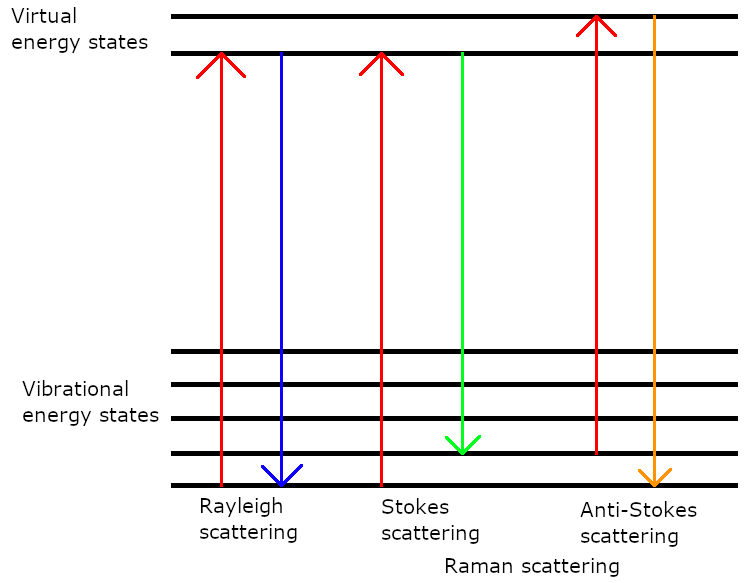
\includegraphics[scale=0.3]{Methodology/RamanEnergyLevels.png}
		\caption{An energy diagram comparing elastic and inelastic scattering. Reproduced from en.wikipedia.org}
		\label{fig:MethodologyRamanEnergyLevels}
	\end{center}
\end{figure}

The phonons that are emitted or absorbed during the transitions between the virtual states in the Raman effect are phonons of the vibrational modes in the material. For any solid state crystalline material the point group can be defined. Using the point group the available vibrational modes can be found. In order for Raman scattering to occur a change in polarisability must occur in a given vibration mode. Similarly if the vibrational mode results in change in dipole moment it results in an IR active mode. As a result a set of available Raman active modes can be found. The Raman spectrum can be therefore used to identify the vibrational modes and therefore gain insight about various factors that influence those vibrational modes.

A typical Raman spectroscope setup involves a monochromatic light source, generally a laser, which is focused on a sample. As a result some of the light is scattered elastically (Rayleight scattering) while even smaller part is scattered inelastically (Raman scattering). The scattered light is then passed through a filter to remove the elastically scattered light at the wavelength equal to that of the incident photons. The remaining Raman scattered light is passed through a monochromator and then onto a CCD detector. A diagram of a Raman spectroscope can be seen in Figure \ref{fig:MethodologyRamanSetup}.

\begin{figure}[!h]
	\begin{center}
		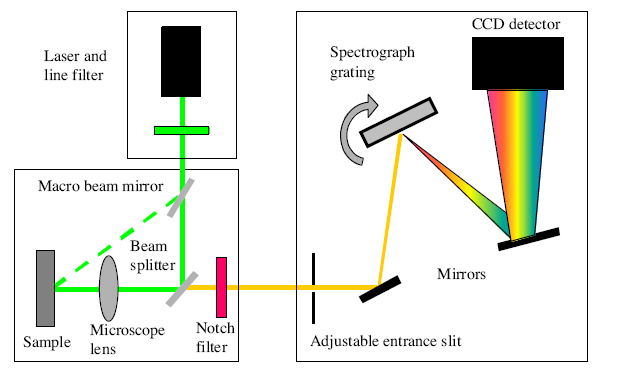
\includegraphics[scale=0.7]{Methodology/RamanSetup.png}
		\caption{A typical Raman spectroscope setup. Reproduced from www.sas.upenn.edu}
		\label{fig:MethodologyRamanSetup}
	\end{center}
\end{figure}

A Raman spectrometer used in this work is a Renishaw Raman spectrometer. The 532nm laser was used as a light source in a backscattering geometry. Unless otherwise specified the measurements were taken at room temperature and ambient pressure. An objective lens of 100x with 0.9 numerical aperture was used as the focusing lens. The laser power was set to be 1.6mW with 0.1s acquisition time for mapping and 1s acquisition time for single spectra. The grating of 1800 lines/mm was used resulting in a resolution of about 1.5 $cm^{-1}$. For calibration purposes a silicon sample was used with a peak at 520 $cm^{-1}$. All data analysis was performed using MATLAB software. The peak fitting script used has been attached in Appendix \ref{app:Matlab}.

\section{Photoluminescence spectroscopy}

The photoluminescence spectroscopy (PL) is an another versatile non-destructive characterisation technique. When applied to the 2D TMDCs it can provide great insight into the crystal stricture, electronic structure of the material as well as some direct information about its optical properties. One of the great advantages of PL spectroscopy is shared with the Raman spectroscopy in that the sample preparation and handling is very easy and quick allowing for high throughput of characterisation. Unlike Raman spectroscopy a substrate choice might become more important for PL measurements owing to the fact that the conductive substrate might result in PL quenching. Since the bandgap of many of the 2D TMDCs lies within the optical range of the spectrum or near to it a single laser at 532nm can be used to excite the samples.

Photoluminescence is a type of luminescence where an excitation is provided by the incident light. In a semiconducting material like many of the 2D 2H TMDCs the electron from valence band is excited to the conduction band. Following the excitation the electron and resulting hole relax in both energy and momentum to the edge of the conduction and valence band respectively. Thus they form an exciton, a quasi particle that contains no net charge and can move across the material. An exciton in TMDCs can approach large sizes (Wannier-Mott exciton) due to great value of dielectric constant and resulting screening between the electron and the hole. Such exciton can also interact with the material by getting pinned by defect sites. After very short lifetime the exciton recombines emitting the photon at the same time. The photons emitted by the recombining exciton can be then collected. A plot of the photon count versus the energy of the detected photon forms the PL spectrum.

Therefore the PL spectrum can be used to directly infer the optical bandgap which is the electronic band gap of the material minus the binding energy of the exciton. In TMDCs on top of excitons additional type of quasi particle like trions or biexcitons can be found. Those particles exhibit varying level of binding energy and sometimes require special conditions to become excited. The PL spectrum can be therefore used to infer about the presence of those particles and therefore gain insight into the structure of the material. An energy diagram representing the photoluminescence (fluoresecence) process can be seen in Figure \ref{fig:MethodologyPLDiagram}.

\begin{figure}[!h]
	\begin{center}
		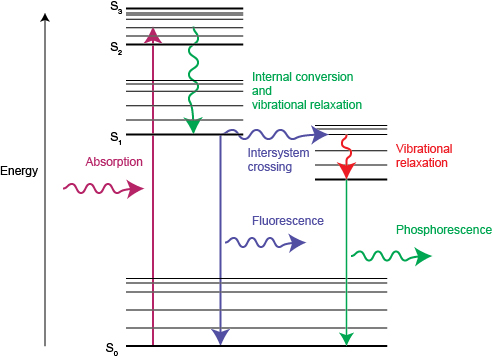
\includegraphics[scale=0.7]{Methodology/PLDiagram.png}
		\caption{The photoluminescence (fluorescence) process. Reproduced from www.renishaw.com}
		\label{fig:MethodologyPLDiagram}
	\end{center}
\end{figure}

The PL signal becomes broadened due to variety of factors. On of the most important contributors is temperature which results in Gaussian broadening. At room temperature there is a constant peak broadening of about 25 meV. Because that broadening is relatively close to the binding energy of the trion ($\sim$30 meV). Therefore at room temperature the trion peak which is generally weaker than the exciton peak cannot be easily resolved. In order to be able to resolve those peaks a PL measurement at lower temperature can be performed.

A photoluminescence setup can look very similar to that of the Raman setup as seen in Figure \ref{fig:MethodologyRamanSetup}. A monochromatic light source e.g. a laser illuminates the sample at the energy greater than that of the materials bandgap. As a result of that the photons emitted from the material together with the inelastically (Raman) and elastically (Rayleigh) scattered photons pass through a filter to remove the latter. The remaining light is then passed through monochromator and detected at the CCD detector. As a result the PL and Raman spectra can be observed in the same spectrum, provided that the sample material can produce both of those signals. 

For low temperature (77K) measurements an environmental stage, Linkam THMS-350V. A pump was used to lower the pressure in the chamber down to about $2 \times 10^{-3}$ mbar. The liquid nitrogen was used to cool down the stage down to 77K. The stage was placed in Renishaw Raman spectrometer to capture PL spectra.

The PL spectrometer used in this work is a Renishaw Raman spectrometer. The 532nm green laser with objective lens of 100x with 0.9 numerical aperture was used and the data was recorded in backscattering configuration. The laser power used was 0.32mW with 0.1s exposition time for maps and up to 5s exposition time for a single extended spectrum. The 1800 lines/mm grating was used resulting in a resolution of about 1.5 $cm^{-1}$. The spectrum was calibrated using silicon Raman peak at 520 $cm^{-1}$. All data analysis was carried out was done using MATLAB software and the peak fitting script can be found in Appendix \ref{app:Matlab}.

\section{X-ray photoelectron spectroscopy}

One of the most useful characterisation techniques for study of 2D TMDCs is X-ray photoelectron spectroscopy. It is a non-destructive method which allows to gain information about the chemical composition of the studied material. It is a very surface sensitive method that allows for obtaining signals from about 10 nm of the sample depth. In order to perform the XPS measurement the sample must be placed in high vacuum (about $10^{-8}$ mbar). It is therefore necessary that the sample contains no liquids or adsorbed gasses which would increase the pressure inside the analysis chamber. 

When a sample is irradiated with a beam of x-ray photons some of those photons get absorbed by the electrons in the sample. Because the energy of the incident photons is relatively large the electrons have enough energy to leave the atoms and travel towards the detector. At the detector their kinetic energy is measured. Because the energy of the incident x-ray photons is known and the kinetic energy of the photoelectrons is measured the remaining energy can be calculated using Equation \ref{eq:XPSEquation}:

\begin{equation}
E_{binding}  = E_{photon} - (E_{kinetic} + \Phi)
\label{eq:XPSEquation}
\end{equation}

If the $\Phi$ which is a instrumental correction factor is known then the $E_{binding}$ can be found. This binding energy depends on the specific atoms from which the electron as well as the specific atomic configuration. Because of that the chemical composition of a given sample surface can be determined. Additionally the number of detected electrons is directly correlated to the concentration of the atoms in the given sample the specific atomic percentages within the scanned area can be calculated. The number of detected electrons can be then plotted against the calculated corresponding binding energy of the electrons to form an XPS spectrum. A diagram of the XPS physics can be seen in Figure \ref{fig:MethodologyXPSSetup}.

In TMDCs the XPS can be used to determine the stoichiometric composition of the as grown material as well as detect any traces of unintentional doping from alkali or halogen atoms or intentional doping by e.g. In atoms. Additionally the amount of oxides as well as the presence of 2H or 1T phases can be quantitatively determined. 

The XPS spectra were collected using the Thermo Scientific K-Alpha XPS system. The Al $K_{\alpha}$ emission line was used as the x-ray source. The pass energy of 20 eV and the energy step of 0.1 eV were used. The XPS spectra were collected at room temperature and pressure of about $3 \times 10^{-8}$ mbar. The acquired data was analysed using Avantage software.

\begin{figure}[!h]
	\begin{center}
		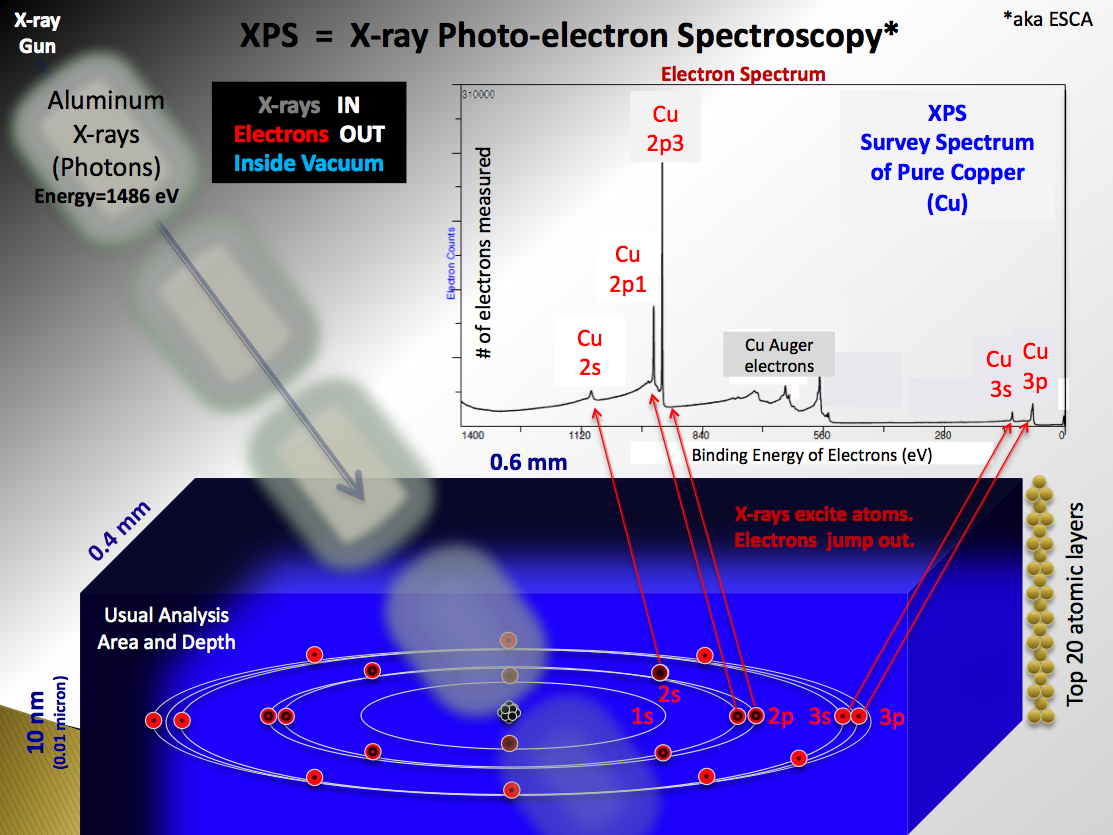
\includegraphics[scale=0.3]{Methodology/XPSSetup.png}
		\caption{XPS spectrum acquisition diagram. Reproduced from en.wikipedia.org}
		\label{fig:MethodologyXPSSetup}
	\end{center}
\end{figure}

\section{Transfer}

Due to the nature of the 2D materials, the 2D TMDCs are generally always deposited on some substrate and cannot be used independently of it. Depending on the manufacturing method different substrates can be used to initially synthesise or deposit the material. In general however the initially used substrate is different to that which can be used for either characterisation or specific application. The samples synthesised by CVD are grown generally on $Si/SiO_2$ at very high temperature and as such cannot be readily used in electronic applications due to $Si$ deterioration at high temperature. To that effect the as grown samples are required to be transferred to a new substrate. 

In this work the wet transfer method has been utilised to transfer CVD grown samples from $Si/SiO_2$ to another $Si/SiO_2$, Au or TEM grid substrate. In this method the sample is first spin-coated with a thin layer of PMMA at 3000 RPM for 60 s. After that the sample is dried and heated up to about 50 {\degree}C for about 1 hour to ensure full polymerisation. Following that the substrate with the sample is then placed in a bath of 8\% KOH solution for about 45 min or until the $Si$ under the $SiO_2$ has completely sank to the bottom of the beaker. The thin layer of PMMA with the sample at the bottom is then scooped up with a glass slide and transferred to a DI water to remove the KOH. The sample is held in a water bath for about 30 min and the step is repeated 2-3 more times. After the last dilution step the sample is scooped onto a target substrate. The sample is then gently dried using compressed nitrogen or air to drive any water from between the PMMA and the substrate. The substrate is then heated up to about 50 {\degree}C for about an 1h to completely dry the sample of any water and ensure better adhesion to the substrate. The substrate is then placed in a bath of acetone and isopropanol heated up to 60 {\degree}C for about an 1h to remove the PMMA layer. After all PMMA has been removed the sample is heated again on a hot plate up to 100 {\degree}C to remove any traces of PMMA.

\section{Device fabrication}

In order to measure the electric properties of the as-grown materials the material can be used to make a field effect transistor (FET) device. For that purpose the as grown mono- and bi-layer $WS_2$ was transferred onto a $Si/SiO_2$ substrate with the $SiO_2$ layer of 285 nm in thickness. The $Si$, which is highly p-doped, then acts as a global gate electrode while the $SiO_2$ is a gate dielectric. On top of the deposited contacts for source and drain electrodes additional probes were used in each of the FET devices to eliminate any voltage contributions from the contacts and thus allow for correct measurement of the channel conductance. The drain and source drains as well as the voltage drains were deposited using electron beam lithography. The contacts as well as the probes were made using 50 nm thick Au, while the rest of the leads were made using 5nm thick Ti and 50 nm thick Au. Following the contacts and leads deposition the FET devices were annealed at 200 {\degree}C fpr 2h under $H_2/Ar$ (10/90) flow at 1 bar to remove any remaining PMMA from the lithographic process. The sample was then annealed at 115 {\degree}C for 60 h under high vacuum ($10^{-6}$ mbar) to remove any remaining water.

Following the FET preparation the samples were then characterised in a vacuum chamber in high vacuum ($10^{-6}$ mbar). A low noise source-meter was used to bias the drain electrode with source being grounded. Additionally another source was used to bias the gate electrode. The current across the channel $I_(ds)$ was measured using ammeter while the voltage $V_{A-B}$ across the voltage probes was measured with a voltmeter. The gate bias was applied until the measured current reached linear regime where it is described by Equation \ref{eq:FETCurrent} \cite{Sze2006}: 

\begin{equation}
I_d = {\mu}_nC_{Ox}\frac{W}{L}(V_{gs} - V_{th})V_{ds}
\label{eq:FETCurrent}
\end{equation}

where ${\mu}_n$ is electron field effect mobility, $C_{Ox}$ is the $SiO_2$ capacitance, W, L are the channel width and length, $V_{th}$ is the threshold voltage, $V_{ds}$ and $V_{gs}$ are the drain-source voltage and gain-source voltage respectively. From the measurement of the current the field-effect mobility for the mono- and bi-layer of the $WS_2$ can be calculated using the linear part of the plot from Equation \ref{eq:FETMobility}: 

\begin{equation}
\mu_{n} = C_{Ox}^{-1}\frac{d{\sigma}}{dV_{gs}}
\label{eq:FETMobility}
\end{equation}

where $\sigma$ is the channel conductivity which can be calculated from Equation \ref{eq:FETConductivity}:

\begin{equation}
\sigma = \frac{LI_{ds}}{W V_{A-B}}
\label{eq:FETConductivity}
\end{equation}

and the oxide capacitance $C_{Ox}$ was calculated to be 115$\mu F m^{-2}$ using Equation \ref{eq:FETCapacitance}:

\begin{equation}
C_{Ox} = \frac{{\epsilon}_0{\epsilon}_r}{d_{Ox}}
\label{eq:FETCapacitance}
\end{equation}

where ${\epsilon}_0$ and ${\epsilon}_r$ are the vacuum and relative permittivity of $SiO_2$ respectively and $d_{Ox}$ is the oxide thickness \cite{Sze2006}.

Additionally the the resistance vs temperature measurements were performed flakes were contacted using two wires configuration. The contacts were deposited using standard photolithographic method by applying the photo resist mask (AZ 5214E) followed by evaporation of Ti (5 nm) and Au (30 nm) using thermal evaporation and sputtering respectively. The measurements were then performed using six arm cryogenic probe station. The measurements were taken at high vacuum of $10^{-5}$ mbar and liquid nitrogen temperature. Following the measurements the conductivity was calculated from $\sigma = \frac{L}{RA}$, where L is the distance between contacts ($\sim$3 $\mu m$), R is the resistance while A is the flake cross section (0.9 nm - 40$\mu m$). The Keithley 2410 source measure unit as well as Lakeshor temperature controller were used for the measurement.

\section{Scanning electron microscopy (SEM)}

Scanning electron microscopy (SEM) is a versatile technique that allows for high resolution imaging of the sample surface. The fundamental operation of the SEM is based on a high energy (1 - 30 keV) electron beam which is rastered across the surface sample under high vacuum ($<10^{-5}$ mbar). The incident beam then is scattered by the atoms producing backscattered electrons, secondary electrons, Auger electrons, characteristic x-rays, fluorescent x-rays and continuum x-ray. The backscattered electrons (BSE) are those electrons that undergo elastic scattering during the process and are then measured by the detector. Similarly the secondary electrons (SE) are those electrons that undergo the inelastic scattering and can then, using a different detector to the BSE, can be detected and counted. The depth from which the BSE are detected ranges up to $\sim$100 nm while that of the SE is limited to $\sim$10 nm.

The SEM images were produced using field emission gun SEM (FEG-SEM, Gemini 1525) with an In-Lens SE detector. The FEG-SEM allows for narrower spot size ($<5 nm$) and a higher signal to noise ratio compared to the conventional thermionic emitters utilised in SEM \cite{Ogura2009}. Due to the thickness of the $WS_2$ the SE were primarily used for imaging. Due to the position of the In-Lens SE detector in the electron column with a rotational symmetry around the optical axis it allows for use of low energy ($\sim$1 - 5 keV) for acceleration and close distance. Because of that the contrast between different number of layers can be achieved for some 2D materials \cite{Kochat2011}. However in order to maintain good signal to noise ratio a slightly higher energy (5 - 10 keV) was utilised.

\begin{figure}[!h]
	\begin{center}
		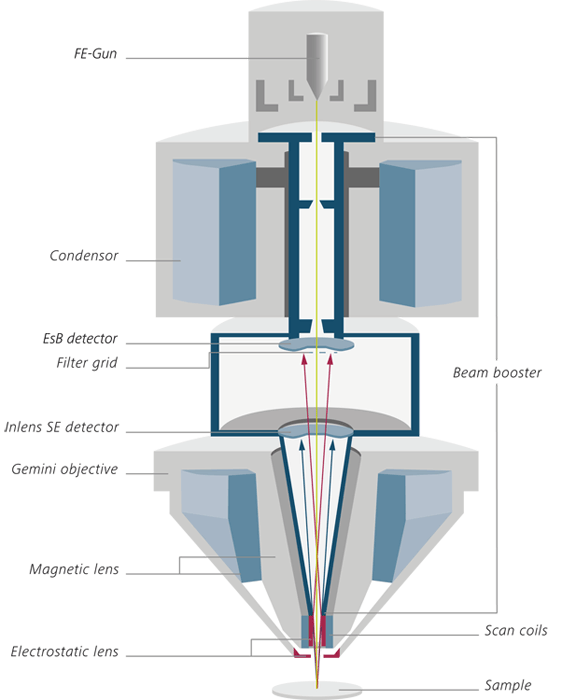
\includegraphics[scale=0.3]{Methodology/SEMSetup.png}
		\caption{Cross section of the SEM optical column. Reproduced from zeiss.com}
		\label{fig:MethodologySEMSetup}
	\end{center}
\end{figure}

\section{Atomic force microscopy (AFM)}

The atomic force microscopy (AFM) is one of scanning probe microscopy methods that allows for imaging surface morphology below the nm range as well as manipulation and force measurement. As seen in Figure \ref{fig:MethodologyAFMSetup} the AFM operates by touching and following the sample surface. The probe, which is a very sharply ended tip made of silicon or silicon nitride and a tip radius in the range of nanometers, is mounted on a cantilever. That cantilever is then controlled by a piezoelectric actuator which adjust the position based on the feedback from the laser measuring the actual cantilever deflection. The tip itself when brought close to the surface of the sample experiences a number of possible forces such as van der Waals forces, electrostatic forces, magnetic forces, chemical bond forces or mechanical contact forces which leads to a deflection one way or the other.

\begin{figure}[!h]
	\begin{center}
		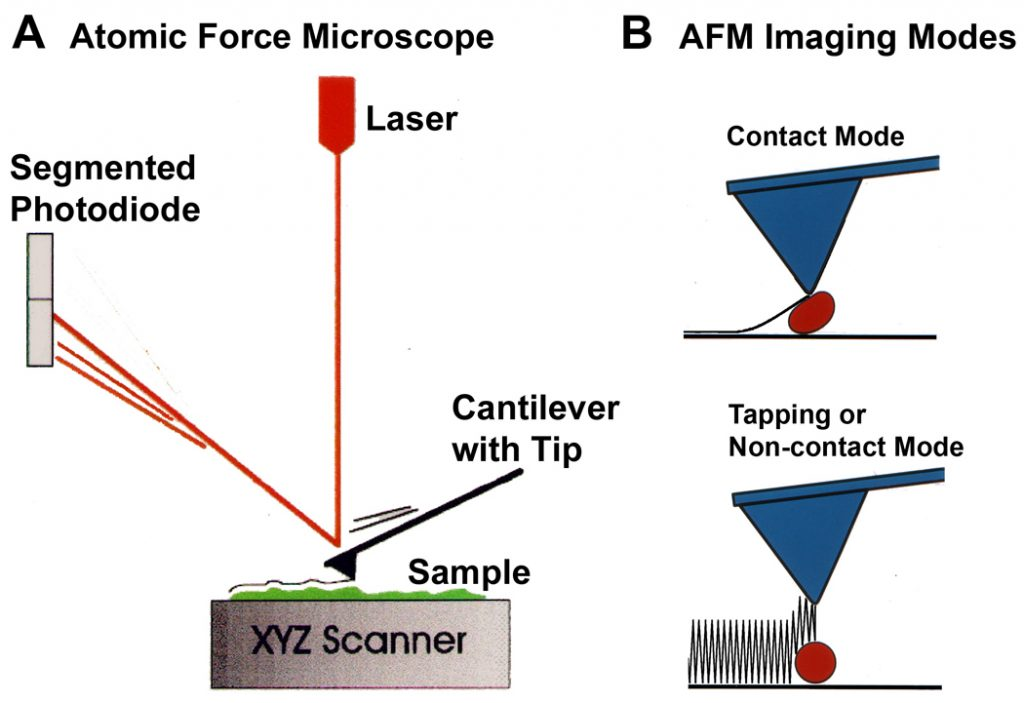
\includegraphics[scale=0.3]{Methodology/AFMSetup.png}
		\caption{Diagram of AFM setup and operating basics. Reproduced from ccem.mcmaster.ca}
		\label{fig:MethodologyAFMSetup}
	\end{center}
\end{figure}

The measurement can be performed in different modes as seen in Figure \ref{fig:MethodologyAFMSetup}. In contact mode the tip is dragged along the surface and either a tip deflection is directly measured or a constant height is maintained while the deflection required to maintain it is recorded \cite{Binnig1993}. Alternatively in a tapping mode the tip is oscillated at a resonant frequency and a constant amplitude is maintained. As the tip gets closer to the surface the forces act stronger and therefore the required correction is recorded and surface morphology and force can be determined. A tapping mode tends to be more useful for characterisation of 2D materials as it avoids damage to them but it is slower and may result in some artefacts \cite{Schmitz1997}.

When using tip with radius of $<$5 nm of curvature a lateral resolution of $\sim$5 nm and a vertical resolution of few \r{A} can be achieved. With a contaminated surface the resolution can quickly become bigger and therefore the thickness measurement of the 2D materials can become overestimated. In this work the measurements were carried out using AFM Asylum MFP 3D in a tapping mode with a probe tip made of silicon nitride and a radius of $\sim$8 nm on a PPP-NCHR 20 Nanosensors cantilever.

\section{TEM}

Transmission electron microscopy (TEM) is a microscopy technique in which a high energy (60-300 kV) electron beam is directed at a very thin ($<$100 nm) sample. As a result an image of the sample can be produced at resolution much greater than that achieved with optical microscopy due to much smaller wavelength of the electrons compared to the visible photons. As the electron beam passes through the sample it carries information about its electron density, periodicity and phase and can then form an image on a fluorescent screen. The resulting bright field image shows contrast due to variation in thickness across the sample, and as the magnification increases the interaction between the electron beam and the sample becomes more complex giving rise to different types of contrast. 

\begin{figure}[!h]
	\begin{center}
		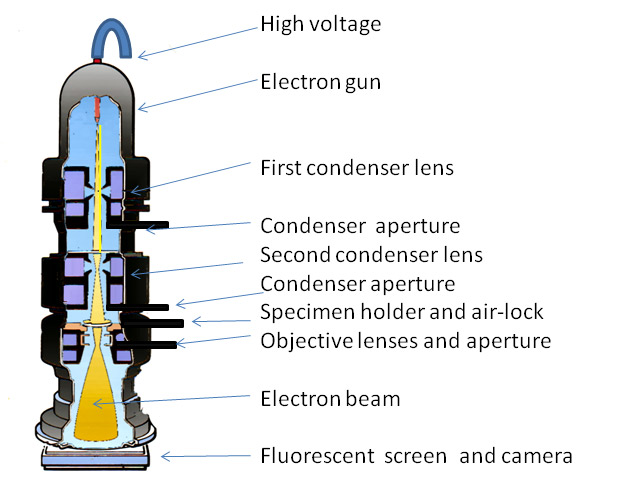
\includegraphics[scale=0.3]{Methodology/TEMSetup.png}
		\caption{Crossection of a TEM column. Reproduced from ccber.ucsb.edu}
		\label{fig:MethodologyTEMSetup}
	\end{center}
\end{figure}

Because the wavelength of the high energy electrons is much smaller than the distance between the atoms in a crystal lattice, the sample can act as a diffraction grating for the incident beam. By shifting the back focal plane instead of the image plane onto the imaging screen and inserting an aperture the diffraction pattern from selected area (SADP) can be achieved. This allows to gain information about the crystal structure and defects within much smaller area than what is possible with x-ray diffraction.

In this work the TEM used was a FEI Titan 80-300 S/TEM at 80kV with a monochromator and $C_s$ aberration image corrector. The focal series images were produced using different objective lens focus values ($C_s = -4\mu m$). Exit wave reconstruction was achieved using TrueImage (FEI).

\section{MATLAB Script}

In order to analyse the PL and Raman spectra, both individual and maps, the MATLAB software was utilised. The spectra were exported from the Wire software used for Renishaw Raman spectrometer and they were then imported into MATLAB. Using "peakfit.m" script from "https://terpconnect.umd.edu/~toh/spectrum/peakfit.m" the peaks were fitted with required number of peaks. For peak fitting the Voigt peakshape was used. Several scripts were developed for the purpose of automating data import, analysis and peak fitting of PL and Raman maps.
\section{$WS_2$ CVD state of the art}

One of the major hurdles in development in the field of the TMDCs is the lack of scalable and reproducible method of producing large area samples of TMDCs. One of the most popular method of obtaining samples, especially for the purposes of further research, has been mechanical exfoliation from bulk crystals to single or few layer TMDCs. Said bulk crystals can be found naturally or synthesised using a chemical vapour transport (CVT) method. In this method the precursors are kept in a closed system together with carrier gas and the target substrate and the temperature gradient is applied across the system. The precursor powder (a mixture of metal and chalcogenide precursors) evaporates with the assist of the transport agent to then deposit on the target substrate over the course of days to weeks \cite{Reale2016}\cite{Schmidt2013}. Utilising this method it has been shown that single bulk crystals of $WS_2$, $MoS_2$, $WTe_2$, $MoSe_2$, $MoTe_2$ can be grown \cite{Reale2016}\cite{Schmidt2013}\cite{Al-Hilli1972}\cite{Brixner1962}\cite{Lenz1997}\cite{Brown1966}\cite{Sunil1997}\cite{Lenz1997}. Such grown crystals are then used to produced single and few layer TMDCs by micromechanical exfoliaiton and deposition onto a desired substrate. While as produced thin layers show good optical and electronic properties their size, thickness and distribution are not easily controllable.

Because of that a different method of direct synthesis of thin layers of TMDCs has been used. For the synthesis of $WS_2$ thin films several different W has been considered. The most common W precursor used is a $WO_3$ which tends to produce $WS_2$ samples with very low number of impurities. At the same time however it requires the high temperature ($\sim$1000 {\degree}C) to evaporate and sulfurise. As an alternative with much lower evaporation temperature (~300 {\degree}C) and high volatility the tungsten hexacarbonyl ($WC_6$) can be used. The downside of that precursor however is the potential contamination of the sample with carbon and oxygen. Finally the tungsten halides can form films of high purity, but at the same time their usage results in release of highly corrosive byproducts \cite{Reale2016}. As an alternative to regular CVD the metal organic chemical vapour deposition (MOCVD) has been used to produce uniform $WS_2$ films of $\sim$65 nm thickness using $WC_6$ and $H_2S$ as precursors \cite{Chung1998}.

One of the methods of producing $WS_2$ thin films is a two step process where a thin film of W or $WO_3$ is first deposited onto the substrate and subsequently sulphurised. Those thin films of tungsten can be first deposited using electron beam evaporation or magnetron sputtering. In order to produce thin film of $WO_3$ the as produced W film can be then thermally oxidised. Finally the thin film of W or $WO_3$ is placed in a tubular furnace, like the one used in CVD, heated up to $\sim$800 {\degree}C and exposed to chalcogen atmosphere. As grown $WS_2$ films of up to $\sim$200nm in lateral size from W films retain the distribution and shape of the W films. The $WS_2$ films produced from $WO_3$ films showed triangular growths of up to micrometers in size . This suggests that in case of the sulphurisation of the thin layers of $WO_3$ the W and S species diffuse on the substrate nucleating $WS_2$ triangles and growing to coalesce with other islands resulting in distribution of $WS_2$ domains \cite{doi:10.1021/nn400971k}\cite{Reale2016}.

The CVD approach to growing atomically thin layers of TMDCs have been mostly a single step growth process using metal oxide and chalcogenide powders as precursors \cite{Reale2016}\cite{doi:10.1021/nn4046002}\cite{Cong2013}\cite{Rong2014}\cite{Dumcenco2015}\cite{Lee2012}\cite{Ling2014}\cite{Najmaei2013}\cite{Ji2013}\cite{Zhang2014a}\cite{Yu2013}. For $WS_2$ growth one of the main challenges in this process is a significant difference of vapour pressure between the W and S precursors. It is therefore crucial to carefully control the evaporation rate of both of the precursors to allow for a degree of reproducibility. In order to do that the usual precursors, $WO_3$ and $S$ powders, are placed in separate crucibles in a quart tube in a CVD tubular furnace \cite{Bosi2015}\cite{Shi2015}. Because of great difference in evaporation temperature of S (100-150{\degree}) and $WO_3$ (800 - 1070{\degree}) two separate furnaces are generally used. The growth is generally performed under inert atmosphere of Ar or $N_2$ owing to high reactivity of S when reducing the $WO_3$. The $H_2$ can be introduced into the process to promote the reduction of $WO_3$ which can help regulate the shape of the grown samples from jagged edges to smooth triangles \cite{doi:10.1021/nn403454e}. The synthesis of $WS_2$ can be achieved at both atmospheric pressure as well as low pressure \cite{Bosi2015}\cite{Shi2015}. The low pressure growth condition allows for greater volatility of precursors as well as keeps the substrate free of particulates thus leading to more uniform nucleation. The atmospheric growth can however produce good quality $WS_2$ using metal halides for promoting growth \cite{Li2015}. Thanks to reaction between the metal halides and tungsten oxide species and the subsequent formation of tungsten-oxyhalide species the growth temperature can be brought down to 850 {\degree}C \cite{Li2015}. In order to improve the substrate coverage and produce more flakes on the substrate nucleation promoters have been used. By dropping a solution of perylene-3,4,9,10-tetracarboxylic acid tetrapotassium salt (PTAS) onto the substrate and drying it prior to growth of $WS_2$ a number of PTAS nuclei are formed across the substrate. This promotes the subsequent CVD synthesis of $WS_2$ via heterogeneous nucleation. It also allows for CVD synthesis on a variety of surfaces (sapphire, quartz, silicon) with different surface corrugation \cite{Lee2013}. The growth temperature has also been shown to have great effect on the flake size with a change from 880 {\degree}C to 900 {\degree}C resulting in later size of flakes increasing from $\sim 5 \mu m$ to $\sim 50 \mu m$ \cite{doi:10.1021/nn403454e}. Different approaches to heating the precursors as well as precursor and substrate placement have also been proposed. By placing both $WO_3$ and $S$ precursors in the same furnace, with $WO_3$ in the centre and $S$ at the edge small triangles with anisotropic PL signal across the flake have been observed. The variation in PL has been attributed to S deficiencies resulting from premature evaporation of the S precursor \cite{doi:10.1021/nn4046002}. It has also been shown that by spreading $WO_3$ powder onto one $Si$ wafer positioned in the centre of the furnace and placing target substrate above it and facing it with S precursor in a separate heating element a successful growth can be achieved. The resulting flakes however showed a wide range of both lateral sizes as well as thickness with monolayer flakes showing uniform PL signal across the flake \cite{Cong2013}.  A CVD synthesis was performed on a hBN substrate using $WCl_6$ as a tungsten precursor with flakes up to $3 \mu m$ and narrow PL emission (26 meV) centred around 2.01 eV \cite{doi:10.1021/nn503093k}. In order to grow large area monolayer flakes $WS_2$ Rong et al. has shown that by controlling the S evaporation time and therefore presulphurising the $WO_3$ powders by 10 min flakes of up to 370 $\mu m$ were grown \cite{Rong2014}.

At the same time the CVD growth of $WSe_2$ has proven to be much more difficult. The most common strategy involves the use of $H_2Se$ as the Se source which is a corrosive and extremely toxic gas. Because of that there is need to find substitutes to limit any possible exposure. There has been some successful growths using $Se$ powders but the growth is often limited by low reactivity of Se, especially compared to S \cite{Ahn2017}\cite{Hsu2017}\cite{Li2015}. The resulting flakes therefore tend to be on the size order of 20-30 $\mu m$. There is then room for further study and improvements to achieve bigger flakes with better substrate coverage.

\section{Conclusions}

In conclusion there has been a tremendous push in the area of CVD growth of mono and few layer TMDCs. Especially in case of $MoS_2$ and $WS_2$ many discoveries have been made regarding the mechanism responsible for the nucleation, growth, precursors evaporation and transport. Many strategies however manages often to optimise one parameter at cost of others and therefore no one of those methods can be easily utilised for scalable production for future applications. In case of less popular TMDCs like $WSe_2$ there is even more that needs to be discovered to achieve parity with the established techniques for more common TMDCs.
\chapter{The state-of-the-art of bilayer heterostructure of $MoS_2/WS_2$}

\section{Introduction}

As two-dimensional TMDCs have emerged as promising candidate materials for next-generation electronic and optoelectronic technologies with valley functionalities it has become apparent the need of enhancing some of their properties in view of their applications. For instance, creating band offsets between different monolayer TMDCs would enable efficient separation of charge carriers and rectification of charge flow. This would offer a mechanism for designing devices made by entirely van der Waals atomically thin materials.  Furthermore, the semiconducting monolayer TMDCs — $MoS_2$, $MoSe_2$, $WS_2$ and $WSe_2$ — are also interesting because they possess direct bandgap in the visible region at energy degenerate band edges (valleys), spin–valley coupling and valley-contrasting electronic and excitonic properties.
 The valley physics of TMDC excitons have been intensely studied in the past few years, with recent advances including the optical generation and control of exciton valley coherence. However, as the valley degree of freedom is affected by very fast recombination time (picosecond timescale) would impede any possible exploitation of the valley-functional optoelectronic devices based on valley excitons in monolayer TMDCs in practical applications. The fabrication of bilayered van der Waals (vdW) heterostructures would enable to fully exploit the potential of TMDC in electronic, opto and valleytronic applications.

\section{Properties of bilayer heterostructures}

As it has been explained in Chapter \ref{sec:Introduction}, TMDCs undergo a crossover from indirect bandgap in the bulk to direct bandgap in the monolayer form. As a consequence of this direct band gap, monolayers absorb and emit light rather efficiently. The band structure changes as a function of the number of layers due to the strong interlayer coupling, which results in different shifts in the conduction and valence band edges at various symmetry points in the Brillouin zone as a function of the layer number \cite{WS2BandStructureSimulation}. Vertical TMDCs heterostructures formed by stacking up different monolayers offer a rich collection of physics and functionalities. Theory predicts that any stacked $MX_2$ heterostructures form type II semiconductor heterojunctions and thus it facilitate efficient electron–hole separation \cite{Amin2015}. This would be particularly beneficial for light harvesting and light detection applications. It has been further demonstrated that the charge separation can occurs over ultra fast time scales, such as femtosecond \cite{Hong2014}.
In type II semiconductor heterojunctions, the conduction band minimum and valence band maximum are found in two separate materials. If electrons and holes are photoexcited they will then prefer to stay in different materials. The alignment of electronic bands of $MoS_2$ and $WS_2$ monolayers as predicted \cite{Gong2013} is reported in Figure \ref{fig:HeterostructuresChargeSeperationDiagram}. It shows that monolayer $MoS_2$ and $WS_2$ have bandgaps of ~2.39 eV and ~2.31 eV, respectively, and the $MoS_2$ valence band maximum is 350 meV lower than that of $WS_2$ and the conduction band level is also lower. Thus is this material system, the conduction band minimum resides in $MoS_2$ and the valence band maximum in $WS_2$. This heterojunction structure can lead to efficient charge transfer upon optical excitation with separated electrons and holes residing in two layers. Hong et al has demonstrated that the electron-hole separation occurs in ~50 fs \cite{Hong2014}. The fast separation can be particular beneficial in solar-driven applications such as photoelectron catalysis and solar cells as it reduces the chances of immediate recombination of the charges.
We have demonstrated that the formation of this type of heterojunction of chemically exfoliated $MoS_2$/$WS_2$ and assembled in a form of thin films can be beneficial for photoelectrochemical water splitting. In Chapter \ref{cha:Heterostructures} we discuss the formation of $MoS_2$/$WS_2$ heterostructures in the form of thin films via CVD and their identification via physical characterization. The same structures have been used for photoelectrochemical water splitting. In general, the most studied bilayer heterostructures is formed by $MoS_2$ and $WS_2$ monolayers. This is due to the fact that synthesis of these materials via CVD is better established as compared to the selenides materials. 

\begin{figure}[h]
	\begin{center}
		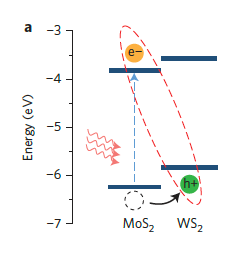
\includegraphics[scale=1]{Heterostructures/HeterostructureChargeSeparationDiagram.png}
		\caption{Charge seperation across heterojunction following photoabsorption. Adoptped from \cite{Hong2014}}
		\label{fig:HeterostructuresChargeSeperationDiagram}
	\end{center}
\end{figure}

\section{Fabrication of bilayer heterostructures}

The first studies of heterostructures of TMDCs have been based on CVD materials. Two different approaches have been adopted. The first strategy was based on the transfer of two monolayers priorly synthesized independently. While the second approach, which has not seen nearly any further work on, was based on the direct synthesis of heterostructures via CVD. 

\subsubsection{Transfer -approach}

$WS_2$/$MoS_2$ heterostructures have been prepared from conventional PDMS stamping method from CVD grown monolayers \cite{Tongay2014}. In the first report about this \cite{Gong2014}, $MoS_2$ and $WS_2$ monolayers have been grown by high-pressure CVD technique onto $SiO_2/Si$ substrates. The CVD $MoS_2$ monolayers were continuous over 1mm with large, single-domain crystals reaching up to 75 microns while the CVD $WS_2$ monolayers were in the form of individual triangle islands of ~5-50 microns in size. 
The fabrication process consisted in a first transfer of the $WS_2$ monolayers onto PDMS substrates, followed by stamping the $WS_2$ monolayers onto CVD $MoS_2$ monolayers, which formed vertical heterostructures of $WS_2$/$MoS_2$ \cite{Tongay2014}. The overlap region (approximately 40 ${\mu}m$) of $MoS_2$ and $WS_2$ monolayers show slightly darker contrast under the optical microscope and it is the region which has been characterized by Raman spectroscopy and photoluminescence and electrical measurements.

\begin{figure}[h]
	\begin{center}
		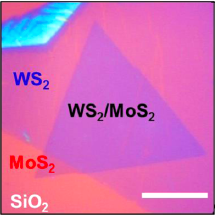
\includegraphics[scale=1]{Heterostructures/HeterostructureOpticalMap.png}
		\caption{Optical micrograph of the heterostructure of $WS_2$/$MoS_2$. Adopted from \cite{Tongay2014}.}
		\label{fig:HeterostructuresOpticalMap}
	\end{center}
\end{figure}

\subsubsection{Direct synthesis of vertical heterostructures}

Firstly, with the term, vertical heterostructures, we differentiate those from the lateral heterojunction created by two adjacent and consecutive layers of two different TMDs.
This terminology differentiates these two different types of heterojunction which can be obtained by direct CVD synthesis.
The direct synthesis of bilayer heterostructures have been obtained via CVD where molybdenum trioxide ($MoO_3$) powder was placed in  front of a bare $SiO_2/Si$ wafer for the growth of $MoS_2$ in a tubular furnace. A mixed powder of tungsten and tellurium was scattered on the wafer for the growth of $WS_2$. A small amount of tellurium was used to accelerate the melting of tungsten powder during the growth \cite{Gong2014}. Upstream in a low-temperature zone, the sulphur powder was placed. The furnace was heated up to the temperature range of 650-850 {\degree}C and argon gas was used as a carrier gas to protect the system from oxygen and carry sulphur vapour from the upstream of the tube during the reaction. The difference in the nucleation and growth rates of $MoS_2$ and $WS_2$ and the chosen growth temperature favours the sequential growth of $MoS_2$ and $WS_2$, instead of  the formation of their ternary alloy ($Mo_xW_{1-x}S_2$ alloy). Vertically stacked bilayers were found to grow preferentially at temperature of ~850 {\degree}C, whereas in-plane lateral heterojunctions were found at ~650 {\degree}C. The CVD  synthesis can lead to clean interfaces \cite{Gong2014}[our paper submitted ] between the two monolayer components, in contrast with mechanical transfer of layers or assembly from liquid phase. A typical optical, SEM and atomic force microscopy (AFM) images of the layers are shown in Figure \ref{fig:HeterostructuresOpticalSEMAFMImages}. The bilayers can be easily distinguished from monolayers via optical contrast (Figure \ref{fig:HeterostructuresOpticalSEMAFMImages}), with $MoS_2$ monolayers showing a light purple colour and the bilayer regions a much darker purple.

\begin{figure}[h]
	\begin{center}
		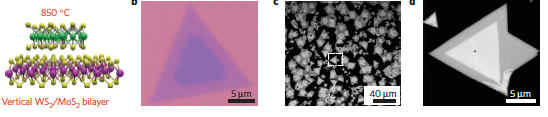
\includegraphics[scale=1]{Heterostructures/HeterostructureOpticalSEMAFMImages.png}
		\caption{Heterostructure imaging. Adopted from \cite{Gong2014}.}
		\label{fig:HeterostructuresOpticalSEMAFMImages}
	\end{center}
\end{figure}

\section{Characterization of bilayer heterostructures}

\subsection{Raman spectroscopy}

Heterostructures fabricated by both these approaches were characterized by Raman spectroscopy. As the vibrational modes of $MoS_2$ and $WS_2$ are quite different the Raman spectrum of the heterostructure displays in-plane ($E^1_{2g}$) and out-of-plane ($A_{1g}$) modes of $MoS_2$ and $WS_2$ at the same frequencies as in their monolayers. The $WS_2$ $E^1_{2g}$ and $A_{1g}$ modes are located at 350 $cm^{-1}$ and 416 $cm^{-1}$ while for $MoS_2$ they are at 380 $cm^{-1}$ and 405 $cm^{-1}$ respectively \cite{Tongay2014}. Spatial maps show consistently distinct signal from each of the two layers using both fabrication techniques (Figure \ref{fig:HeterostructureRamanSpectrumIntro}). In the transferred bilayered heterostructures there is a clear difference  between the Raman modes position of the as transferred materials versus an annealed heterostructure. The position of the peaks for each material in the as transferred materials is compatible with  monolayers while after annealing (at the temperature of 70 {\degree}C) the peaks are affected by redshift/blueshitft as it is characteristics of bilayer materials. This result suggest that as a consequence of annealing (120 {\degree}C at $<$0.13Pa for 6 h) there is an increased interlayer interaction. The fact that no changes are observed in the E modes in plane can be explained with the fact that they are generally less sensitive to changes in the environment. The increased interaction has been also revealed by AFM where the step height of the bilayer heterostructure can be reduced from 1.6 nm toward the expected 0.8 nm by annealing. This can be explained with the possibility that such annealing is able to drive out trapped residual molecules, such as water. In the CVD grown materials, the $A_{1g}$ Raman peaks appears at 418.5 $cm^{-1}$ and 405.3 $cm^{-1}$ respectively for $WS_2$ and $MoS_2$. These values are compatible with a bilayer structures of the annealed transferred samples. This suggest there is an increased interaction between the layers in CVD grown materials in line with layered bulk materials \cite{Tongay2014}.

\begin{figure}[h]
	\begin{center}
		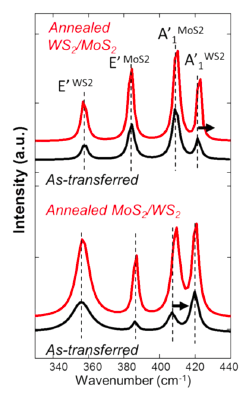
\includegraphics[scale=0.7]{Heterostructures/HeterostructureRamanSpectrumIntro.png}
		\caption{Heterostructure Raman spectrum. Adopted from \cite{Tongay2014}.}
		\label{fig:HeterostructureRamanSpectrumIntro}
	\end{center}
\end{figure}

\begin{figure}[h]
	\begin{center}
		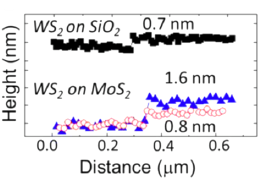
\includegraphics[scale=1]{Heterostructures/HeterostructureAFMProfile.png}
		\caption{Comparison of AFM profiles of $WS_2$ on $Si/SiO_2$ and $MoS_2$. Adopted from \cite{Tongay2014}.}
		\label{fig:HeterostructureAFMProfile}
	\end{center}
\end{figure}


\subsection{Photoluminescence}

\begin{figure}[h]
	\begin{center}
		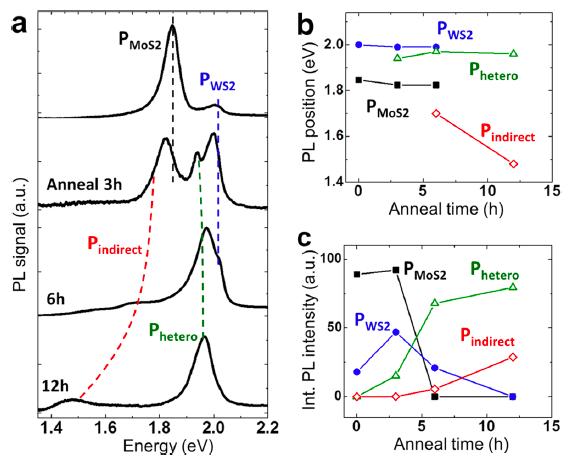
\includegraphics[scale=1]{Heterostructures/HeterostructurePLSpectrumIntro.png}
		\caption{PL Spectrum of heterostructure after annealing. Adopted from \cite{Tongay2014}.}
		\label{fig:HeterostructurePLSpectrumIntro}
	\end{center}
\end{figure}

The vertical heterostructures were further characterized by photoluminescence (PL) spectroscopy.
The as transferred heterostructures manifest PL peak typical of $MoS_2$ and $WS_2$. The spectrum can be defined as additive. The PL peak of $MoS_2$ show intensity much higher $WS_2$ and this was attributed to possibly higher density of defects in $WS_2$ associated with its higher growth temperatures. After annealing the $WS_2$/$MoS_2$ heterostructures, the PL spectrum gradually changes. The transition as seen in Figure \ref{fig:HeterostructurePLSpectrumIntro} from transferred to fully annealed bilayer heterostructures occur through the followings: (1) A new PL peak ($P_{hetero}$) appears at 1.94 eV, and its integrated intensity grows for prolonged annealing time. (2) Upon the annealing, $P_{MoS_2}$ and $P_{WS_2}$ gradually decrease up to the point of appearing as small features at lower and higher energy of the $P_{hetero}$ peak (3) at the end of 12 hours of annealing, another weak emission peak ($P_{indirect}$) appears at 1.75 eV, and the peak position rapidly and eventually red-shifts to ~1.5 eV \cite{Tongay2014}. 

The explanation for this trend has been the following. As a consequence of the transfer the two monolayers end up well separated from each other due to residual water molecules and/or impurities trapped between the sheets. This large distance has been assessed by AFM (Figure \ref{fig:HeterostructureAFMProfile}). This system display PL peaks characteristics of isolated monolayer $MoS_2$ ($P_{MoS_2}$) and monolayer $WS_2$ ($P_{WS_2}$). After the annealing, the PL peak intensity of $MoS_2$ ($P_{MoS_2}$) and $WS_2$ ($P_{WS_2}$) decreases and two new peaks appear, called $P_{hetero}$ and $P_{indirect}$, with the former arising from the electronic coupling between the two monolayer materials while the latter arising due to the indirect band gap formed at the interface of the heterobilayer (Figure \ref{fig:HeterostructurePLSpectrumIntroComparison}). Because the $P_{indirect}$ peak position changes rapidly with the degree of coupling (annealing time). This has been attributed to a phonon-assisted, indirect bandgap transition, which involves the valence band maximum (VBM) at the {$\Gamma$}-point and the conduction band minimum (CBM) at the K-point. To prove this hypothesis, the authors have fabricated by transfer method a $MoS_2$/$MoS_2$ heterostructure and the indirect peak has similar behaviour. This suggested that the indirect peak can be associated with a similar behaviour as the bulk material. DFT calculations has supported this hypothesis \cite{Zande2014}. The formation of a type II heterojunction led to establishing a large electric field which develops across the ~1 nm thick junction. This leads to strong exciton splitting by which holes (electrons) are rapidly swept from $MoS_2$ to $WS_2$ (from $WS_2$  to $MoS_2$).

In order to understand the interlayer interactions DFT simulations have been performed. It has been observed that the twist angle between 2 layers has an effect on several properties of the TMDCs. By twisting the layers from being aligned at 0{\degree} to 30{\degree} the distance between the layers increases by about 0.3 \r{A}. The trend then reverses with distance returning back at 60 {\degree} to the same value as at the 0{\degree}. Additionally it has been predicted that as the twist angle changes from 0{\degree} to 30{\degree} the valence band at K point remains mostly unchanged while the valence band at $\Gamma$ point rises. Due to this the direct transition K-K remains unchanged while the indirect K-$\Gamma$ transition shows lower energy gap. As an explanation of that phenomenon it has been noted that the both valence and conduction band states at K point involve primarily $Mo$ states that are located within the layer. The valence state at the $\Gamma$ point however involves appreciable $p_z$ content of $S$ atoms and $Mo-d_z^2$. Because of that the overlap between those $p_z$ states of $S$ atoms varies significantly with the layer separation \cite{Nayak2017}.

\begin{figure}[h]
	\begin{center}
		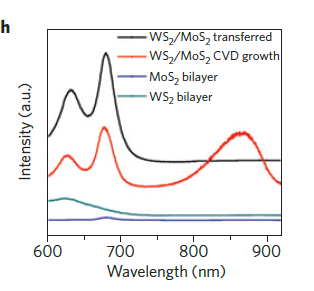
\includegraphics[scale=1]{Heterostructures/HeterostructurePLSpectrumIntroComparison.png}
		\caption{Comparison of PL spectra from hetero and homo bilayers of $WS_2$ and $MoS_2$. Adopted from \cite{Gong2014}.}
		\label{fig:HeterostructurePLSpectrumIntroComparison}
	\end{center}
\end{figure}

The CVD grown heterostructures shows a bandgap of 1.42 eV while at the same time separate pronounced PL peaks of $MoS_2$ and $WS_2$ can be seen (Figure \ref{fig:HeterostructurePLSpectrumInterlayerIntro}) \cite{Gong2014}. Subsequent studies have tremendously developed the understanding of the heterobilayer PL behaviour. The main factor which has been taken into consideration in the following studies is the mismatch angle between the lattices orientations of the two monolayers. Experimentally, it was found that the twist angle in a heterobilayer determines the photoluminescence efficiency of interlayer excitons (bound  electrons and holes situated in adjacent layers) and their peak position. It has been hypothesized that twist-angle-dependent interlayer orbital hybridization can cause the variation in the photon emission energies of indirect excitons in heterobilayers (e.g. $MoS_2$/$WSe_2$) and also in $MoS_2$ bilayers \cite{Nayak2017}. Additional experimental work has reported similar results \cite{Heo2015}\cite{Liu2014a}. 

Specifically, in a study by Kunstamnn \cite{Kunstmann2018} the heterobilayer region of $MoS_2$/$WSe_2$ shows the peaks of the two individual materials are discernible among with a new peak near 1.6 eV. This has been interpreted as the indirect exciton, and renamed as interlayer exciton (ILE). By altering the twist angle between the $MoSe_2$ and $WSe_2$ layers from 0{\degree} to 30{\degree} the ILE peak intensity has decreased and further from 30{\degree} to 60{\degree} the intensity has increased again. Similarly the ILE peak position has blueshifted from 0{\degree} to 30{\degree} and redshifted back from 30{\degree} to 60{\degree}. The separation between the layers is also found to be highest at about 30{\degree} and smallest at 0{\degree} or 60{\degree}. At the same time the other PL peaks, associated with monolayer $WSe_2$ and $MoS_2$, are unaffected. The ILEs can be therefore associated with the K-$\Gamma$ transition.

\begin{figure}[h]
	\begin{center}
		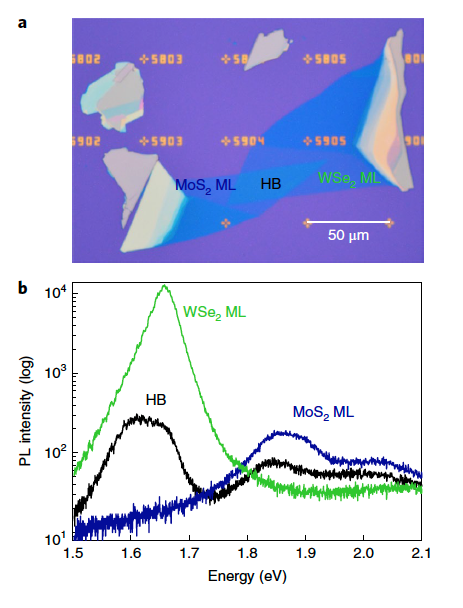
\includegraphics[scale=1]{Heterostructures/HeterostructurePLSpectrumInterlayerIntro.png}
		\caption{PL spectra taken from heterostructure. Adopted from \cite{Kunstmann2018}}
		\label{fig:HeterostructurePLSpectrumInterlayerIntro}
	\end{center}
\end{figure}

Very recently, Alexeev et al \cite{Alexeev2019} have shown the latest achievement in the field consist of bilayered TMDs heterostructures formed by transfer of CVD grown TMD as well as mechanically exfoliated. It has been shown that in the $WSe_2$/$MoS_2$ heterostructure the PL peak associated with $MoS_2$ monolayer redshifts while the one of the $WSe_2$ monolayer remains largely unaffected. Additionally as the twist between the layers increases from 0{\degree} to 60{\degree} the position of that PL peak increases initially and plateaus soon after and drops again near the 60{\degree} twist. It has been then suggested that a strong hybridazation takes place between interlayer and intralayer excitons. The Moir\'{e} pattern formed by twisting the layers results in formation of mini Brillouin zones. Those mini Brillouin zones (mBZ) at small angle twists result in additional interlayer peaks.  Those additional peaks are very strongly twist angle dependent and become less intense and more blueshifted at higher twist angles. 

\begin{figure}[h]
	\begin{center}
		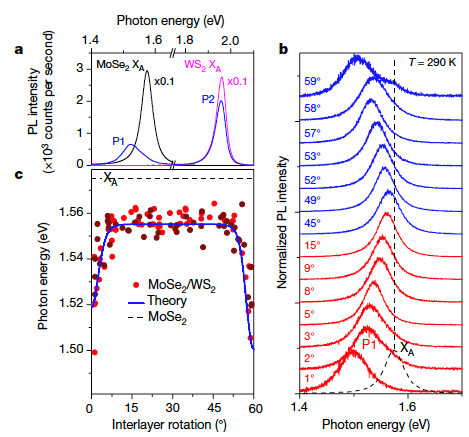
\includegraphics[scale=1]{Heterostructures/HeterostructurePLSpectrumInterlayerTwist.png}
		\caption{PL spectra of heterostructure. Adopted from \cite{Alexeev2019}}
		\label{fig:HeterostructurePLSpectrumInterlayerTwist}
	\end{center}
\end{figure}
\chapter{Polymorphism in group VI transition metals dichalcogenides; a specific case of 1T' and 2H phases of $WSe_2$}

\section{Introduction}

In contrast to other 2D materials like hBN or graphene, TMDCs exhibit structural polymorphism and as such open an additional avenue in 2D material engineering. The relation between different phases observed in TMDCs can be seen in Figure \ref{fig:1T'TMDCPhases}. On top of altering the electronic nature of the TMDC, semiconducting or metallic, there can also be observed a variety of superconducting states \cite{Saito2015}\cite{Lu2015}, quantum spin Hall insulators \cite{Qian2014}\cite{Choe2016}\cite{Liu2016a}\cite{Fei2017} or Weyl semimetals \cite{Sun2015}. Interestingly the various TMDC phases can coexist at specific temperatures and pressures \cite{Kappera2014}\cite{Keum2015}\cite{Cho2015}. Those different phases can exhibit small difference in energy per formula unit $MX_2$. As such a phase transition can be induced via e.g. a charge injection \cite{Duerloo2014}. Overall the various phases of the TMDCs and the transitions between are of great interest and remain unexplored in full detail.
The monolayers of TMDCs can be usually found in either 1H or 1T phase where the exact configuration depends on the thermodynamics \cite{Keum2015}\cite{Cho2015}. In order to identify which of those phases is more favourable the crystal field theory can be applied. The number of electrons in d orbitals of transition metals needs to be counted for a given TDMC material. For group 4 TMDCs (Ti, Zr and Hf) that number is 0 ($d^0$) while for group 10 (Ni, Pd and Pt) the number is 10 ($d^6$). It can be therefore shown that the number of electrons in d orbitals correlates with the phase transitions in TMDCs as seen in Figure \ref{fig:1T'EnergyDiagram}. The group 4 TMDCs ($d^0$) for instance are most stable in 1T phase. However the $d_{z^2}$ level of the 1H phase has the lowest energy and therefore the TMDCs of group 5 ($d_1$) and group 6 ($d_2$) fill that level first and therefore, they group 5 TMDCs are found most stable in  either 1T or 1H phase while the group 6 TMDCs are most favourable in 1H. After filling the $d_{z^2}$ level in group 6 TMDCs, the additional electron in group 7 TMDCs contribute to the 1T levels and results in a distorted octahedral coordination (1T') with clusterisation or Peierls distortions of the metal atoms. Furthermore the group 9 and 10 TMDCs are most stable in the regular octahedral coordination (1T).

\begin{figure}[!h]
	\begin{center}
		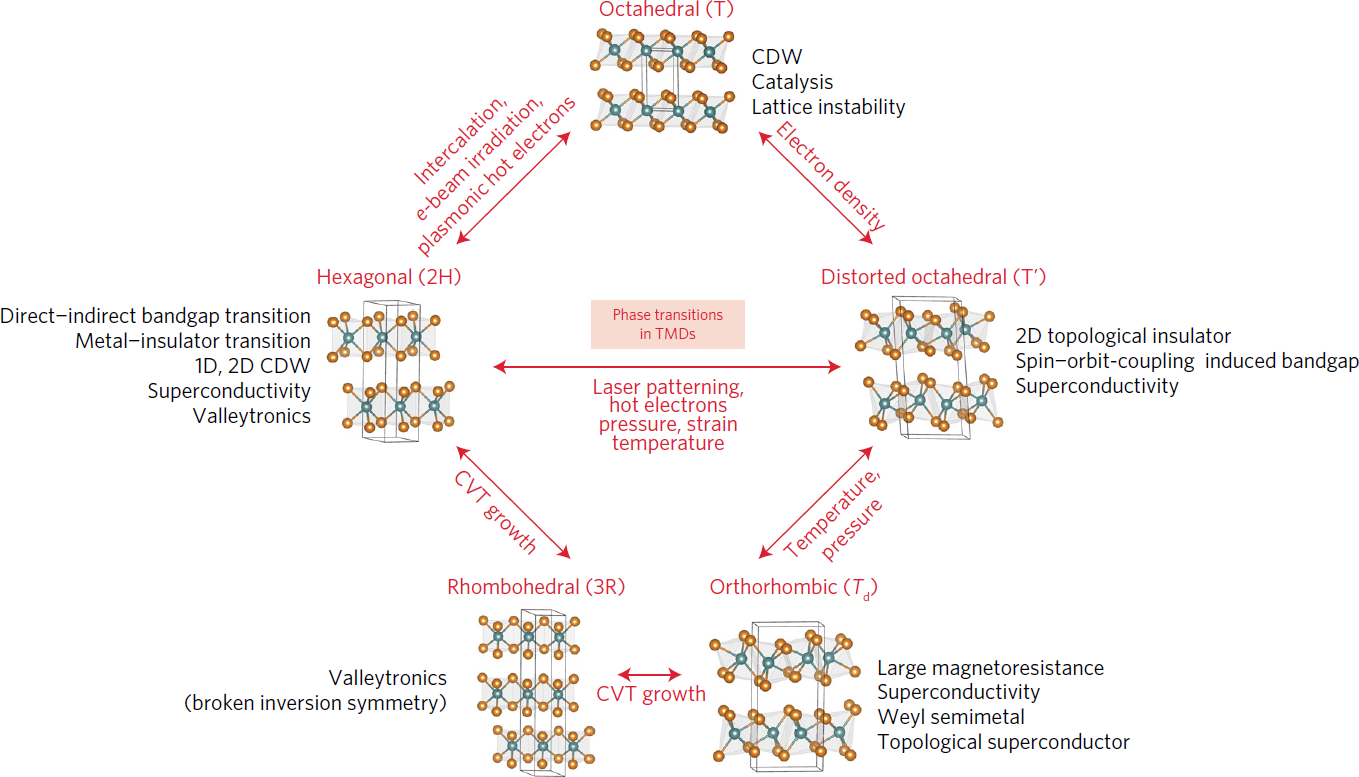
\includegraphics[scale=0.3]{1T'/TMDCPhases.png}
		\caption{Transition and correlation between phase and physics in TMDCs. Reproduced from \cite{Yang2017}}
		\label{fig:1T'TMDCPhases}
	\end{center}
\end{figure}

\begin{figure}[!h]
	\begin{center}
		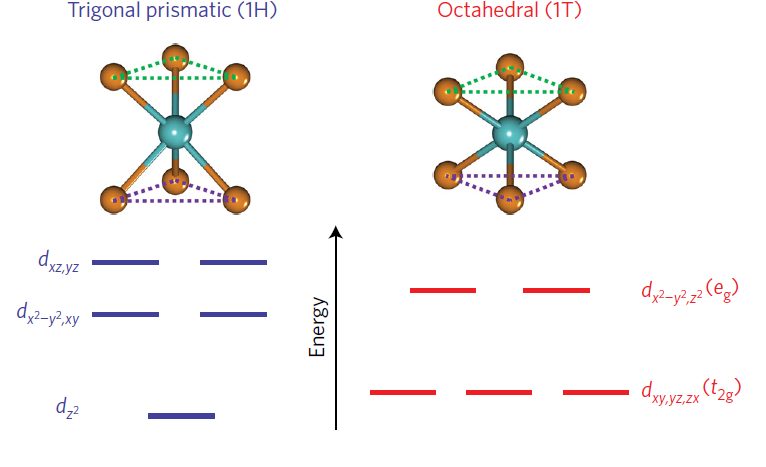
\includegraphics[scale=0.5]{1T'/EnergyDiagram.png}
		\caption{Schematic images of 1H and 1T lattice symmetries and energy levels of d-orbital electrons induced by the crystal field. Reproduced from \cite{Yang2017}.}
		\label{fig:1T'EnergyDiagram}
	\end{center}
\end{figure}

Recently the 1T' phase has received attention due to the predictions of potential Weyl semimetal or quantum spin Hall effects for group 6 TMDCs \cite{Qian2014}\cite{Sun2015}. Additionally the lattice distortion orientation can be affected by strain which allows for mechanical control of ferroelasticity and potential application as a shape memory material \cite{Li2016}. In order to achieve those effects in group 6 TMDCs a phase transition from 1H to 1T' generally has to be occur \cite{Chhowalla2013}. Such transition is usually performed via the lithium intercalation or chemical exfoliation. Following the lithiation the excess of the electrons is found in the d orbitals of the transition metals. As a result of that the electron density of those orbitals increases from $d_2$ to $d_{2+x}$. In order for a full transition from 1H to 1T to occur the excess of the electrons must be in range of 0.2 to 0.4. However if the excess is smaller than that then the distortion of the lattice may help to accommodate the phase transition.

One of the most important characteristics of TMDCs that influences a myriad of different properties is the number of layers. Especially in case of optical and electronic properties of 2H TMDCs the number of layers strongly affects the size and the nature of the bandgap, transitioning from indirect in bulk to direct in monolayer. The number of layers is however also of crucial importance to quantum effects observed or predicted in TMDCs in that the bulk material exhibits the in-plane inversion symmetry while the monolayers break it \cite{Saito2015}\cite{Lu2015}. Such breaking of symmetry leads to strong spin-orbit coupling as well as effective Zeeman fields in TMDCS. Additionally and out of plane spin polarisation which depends on the valley, K or -K point, has been observed when a strong anisotropic magnetic field has been applied to quench the superconductivity in 2H-$MoS_2$. There has also been observed a superconducting state in monoclininc and 1T' $MoTe_2$, and where also the Weyl semimetal and topological insulator states are expected \cite{Qian2014}\cite{Sun2015}\cite{Qi2016}.

Due to the distortion in the 1T' phase of the group 6 TMDCs a band inversion near the Fermi level with p and d bands from chalcogenides and metal atoms respectively. These bands result in some interesting phenomena, the Weyl state and quantum spin Hall effect. Those effects can manifest themselves in distorted octahedral phase (1T') or ortorhombic ($T_d$) phase. It has been shown using DFT calculations that group 6 TMDC in the T' phase exhibit the band inversion resulting in the quantum spin Hall effect \cite{Qian2014}\cite{Choe2016}. The change in number of layers results not only in inversion symmetry breaking but also affects the bandgap magnitude and as such is crucial in achieving the dissipationless spin transfer by the QSH \cite{Kane2005}\cite{Konig2007}. It has theorised that a topological FET can be realised through the application of the external electric field which can turn the topological states on or off.

In contrast to the 1T' phases of group 6 TMDCs, the orthorombic $T_d$ phase shows Weyl semmimetalic states as a result of the inversion symmetry breaking. The $T_d$ phase can be achieved via control of the defects, cooling down the T' phase below 240K or as a result of high pressure \cite{Qi2016}. 

A phase transition from 2H to 1T in $MoS_2$ has been observed using the TEM. Several intermediate phases have been identified and the gliding planes of Mo and S atoms have been observed. It has also been shown that the electron injection in TEM can be used to pattern the phase transition, and therefore that the electron driven phase transition is possible \cite{Lin2014}. Additionally it has been shown that local heating and the chalcogenide defects created as a result can induce an irreversible transition from hexagonal to monoclinic phase in $MoTe_2$ \cite{Cho2015}. A laser irradiation can also cause a phase transition in $MoS_2$ from monoclinic to hexagonal, where the activation energy for the transition has been found to be ~400 meV \cite{Guo2015}. There has also been demonstrated transition from hexagonal to monoclinic $MoS_2$ using plasmonic hot electrons \cite{Kang2014}. The injected hot electrons in the 4d band of the Mo atoms result in a more stable monoclinic phase according to the crystal field theory. As one of the potential application an infrared sensor can be proposed where a phase transition is engineered by strain to occur at such low temperature that a small change in temperature can induce it \cite{Song2015}.

A contact between the 2D TMDC layer and rest of the device is of critical importance for any electronic and energy application. The commonly used transfer method of assembling the material with the contacts is generally undesirable as it alters the structure of the TMDC material. To this effect the homojunction offers a viable alternative as it has been presented with local transition from 2H $MoS_2$ to 1T $MoS_2$ \cite{Kappera2014}. The resulting 1T metallic phase interface as seen in Figure \ref{fig:1T'Homojunction} with the metal contacts reduces the contact resistance in $MoS_2$ FET.

\begin{figure}[!h]
	\begin{center}
		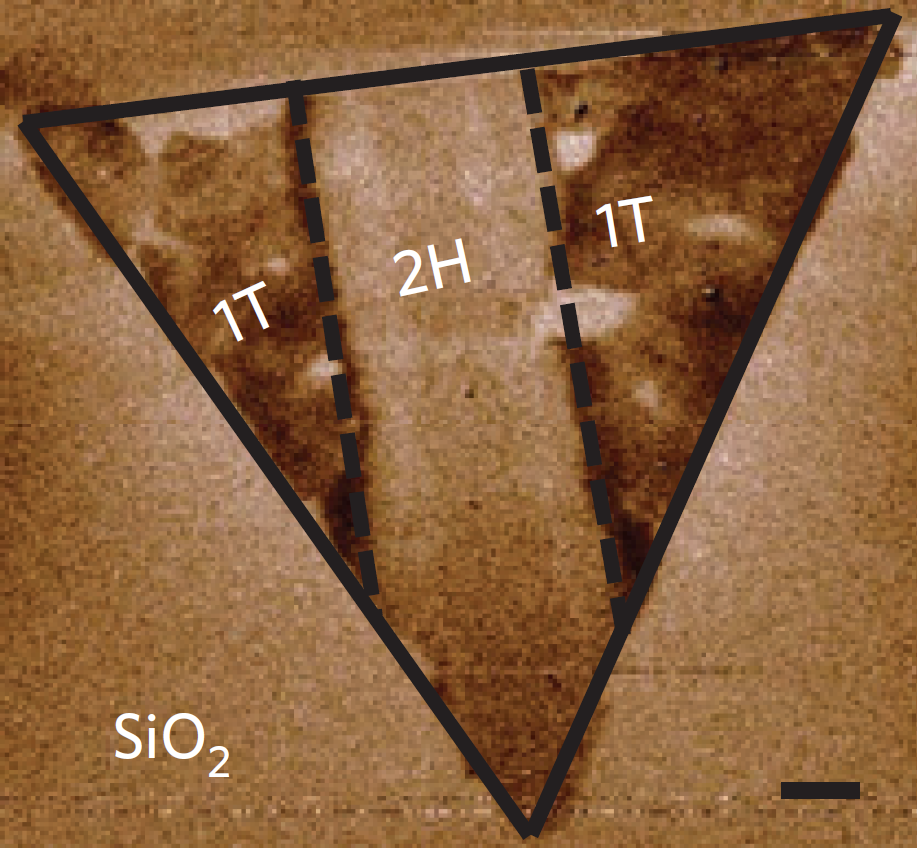
\includegraphics[scale=0.25]{1T'/Homojunction.png}
		\caption{Electrostatic force microscopy phase image of a monolayered MoS2 homojunction. Reproduced from \cite{Kappera2014}}
		\label{fig:1T'Homojunction}
	\end{center}
\end{figure}

\section{Conclusions}

In this chapter we have summarized the fundamental differences between 2H and 1T/1T’ phases of TMDCs with emphasis on the different crystalline phases and electronic properties along with different phenomena that can be enabled by the 1T’ phases. Additionally, we have laid out a short summary of the synthesis methods for the metastable 1T/1T’ phases.
\chapter{Role of precursors in growth of monolayer $WS_2$}

In this chapter the CVD growth of $WS_2$ using different precursors is investigated. The as grown samples were characterised by Raman and PL spectroscopy as well as XPS, XRD, AFM and electrical measurements. As a result it was concluded that using $H_2WO_4 + NaCl$ at 850 {\degree}C gives best results. Such grown samples exhibit biggest flakes up to 200 $\mu m$ in size as well as show the strongest and most narrow PL peak with 36 meV FWHM. The samples grown using $H_2WO_4 + NaCl$ at 950 {\degree}C show also best transistor electron mobility in monolayer CVD grown $WS_2$ while that grown using $WO_3 + NaCl$ at 950 {\degree}C shows best transistor electron mobility in bilayer CVD grown $WS_2$. 

\section{Introduction}
	
Monolayers of transition metal sulphides and selenides exhibit range of interesting properties such as strong light absorption in the IR and visible range \cite{AtomicallyThinMoS2ANewDirect-GapSemiconductor}\cite{ExtraordinarySunlightAbsorptionAndOneNanometerThickPhotovoltaicsUsingTwo-DimensionalMonolayerMaterials}\cite{EvolutionOfElectronicStructureInAtomicallyThinSheetsOfWS2AndWSe2}, valley polarisation \cite{ControlOfValleyPolarizationInMonolayerMoS2ByOpticalHelicity} \cite{ValleyPolarizationInMoS2MonolayersByOpticalPumping}, spin-orbit interactions \cite{CoupledSpinAndValleyPhysicsInMonolayersOfMoS2AndOtherGroup-VIDichalcogenides}\cite{GiantSpin-orbit-inducedSpinSplittingInTwo-dimensionalTransition-metalDichalcogenideSemiconductors}, tightly bound excitons \cite{TightlyBoundTrionsInMonolayer} or second-harmonic generation \cite{ProbingSymmetryPropertiesOfFew-LayerMoS2Andh-BNByOpticalSecond-HarmonicGeneration}. Some of these effects can be attributed to the lack of free dangling bonds and configuration of d-orbitals \cite{TheTransitionMetalDichalcogenidesDiscussionAndInterpretationOfTheObservedOpticalElectricalAndStructuralProperties}, \cite{ElectronicPropertiesOfMoS2Nanoparticles}.

Among these materials one of the most promising is the $WS_2$. Its visible range bandgap of 2eV as well as an easy and safe manufacturing route via CVD makes it one of the more interesting and studied TMDCs. The typical characterisation by photoluminescence spectroscopy allows to probe the varying synthesis conditions, the grain boundaries or defect population \cite{ExtraordinaryRoomTemperaturePhotoluminescenceInTriangularWS2Monolayers} \cite{doi:10.1021/nn4046002} \cite{Li2015} \cite{Rong2014}. The PL efficiency in as-grown monolayer $WS_2$ produced via CVD growth shows {$\sim$}2-6\% efficiency \cite{doi:10.1021/nn4046002}\cite{Yuan2015} \cite{doi:10.1021/nn403682r}. This efficiency is caused mostly by defect-mediated non-radiative recombination centres \cite{Amani2015}. LEDs have been successfully produced \cite{doi:10.1021/nl500171v} showing external quantum efficiency up to 10\% \cite{Zeng2016}\cite{Withers2015}. $WS_2$ is typically a n-type semiconductor due to the presence of sulphur vacancies \cite{ExtraordinaryRoomTemperaturePhotoluminescenceInTriangularWS2Monolayers}\cite{doi:10.1021/nn5059908}\cite{Iqbal2015}. In order to utilise this material in any potential future applications a reliable and scalable manufacturing method must be developed to ensure a high quality crystal on the wafer scale area. The main method for $WS_2$ synthesis that satisfies these conditions is Chemical Vapour Deposition (CVD) \cite{Hofmann1988}. The growth of tungsten based TMDCs have been less successful than the equivalent molybdenum based TMDCs and has produced mostly isolated flakes of up to 40 $\mu m$ \cite{ExtraordinaryRoomTemperaturePhotoluminescenceInTriangularWS2Monolayers} \cite{doi:10.1021/nn403454e} \cite{Rong2014} \cite{doi:10.1021/nn400971k}\cite{doi:10.1021/acsnano.5b01480}\cite{Fu2015}\cite{Lee2013}. Even larger films of monolayer $WS_2$ have been shown, however they also exhibit low carrier mobility \cite{Kang2015}\cite{Gao2015}. In the typical CVD synthesis process the sulphur and tungsten oxide are evaporated simultaneously in a tubular furnace with a constant flow of carrier gas like argon at temperatures of at least 900 {\degree}C \cite{ExtraordinaryRoomTemperaturePhotoluminescenceInTriangularWS2Monolayers}\cite{doi:10.1021/nn403454e}\cite{Rong2014}\cite{doi:10.1021/nn400971k}\cite{doi:10.1021/acsnano.5b01480}\cite{Fu2015}\cite{Lee2013}. Such growth is predicated by topotacic transformation leading to low density distribution of domains on an amorphous \cite{ExtraordinaryRoomTemperaturePhotoluminescenceInTriangularWS2Monolayers}\cite{doi:10.1021/nn403454e}\cite{doi:10.1021/nn400971k}\cite{Fu2015}\cite{Lee2013} or crystalline substrate \cite{Rong2014}\cite{doi:10.1021/acsnano.5b01480}\cite{doi:10.1021/nn503093k} possibly due to low evaporation rates of $WO_3$. Since $WO_3$ requires high temperatures of 950-1000 {\degree}C to evaporate while the $S$ becomes volatile at 90 {\degree}C the thermodynamics of the process are difficult to control. The low growth dictated by fast evaporation of $S$ leads to limited domain growth and lack of continuous layer. One of the proposed solutions have been to spread the $WO_3$ on the target substrate \cite{doi:10.1021/nn4046002}\cite{Li2015}\cite{Gao2015}\cite{Cong2013}\cite{Yun2015}\cite{Gong2015}\cite{Gong2014}. This has however led to low reproducibility, poor control of thickness and stoichiometry and unreacted material left on the substrate. Another approach has been to use more volatile $W$ precursors such as $WCl_6$\cite{Carmalt2003} or $W(CO)_6$\cite{Kang2015}\cite{Eichfeld2015} together with organic compounds as $S$ precursors. Such method while producing a large area domains at lower temperature has led to lower crystal quality and purity.

Here we propose a different method of CVD synthesis that allows for much larger flake growth of up to 800 $\mu m$ at temperature of 750 {degree}C. Such grown material exhibits high electron mobility in one and two layers of $WS_2$, higher than other values reported in literature. The photoluminescence peak is also very narrow at 36 meV FWHM at room temperature. 

\section{Results}
	
For the purpose of comparing the CVD synthesis method conditions the several sets of precursors were used: $WO_3$, $WO_3$ + NaCl and $H_2WO_4$ + NaCl. The standard growth procedure involves two separate crucibles placed at distance from each other in a quartz tube. Each of these crucibles is independently heated to ensure that the S and the W precursors evaporation rate is maximised at the same time. The vapours then are deposited on $SiO_2/Si$ (285 nm) substrate which is placed close to the W precursor crucible. The entire process is performed under low vacuum and a supply of Ar gas. The furnace setup can be seen in Figure \ref{fig:PaperSIFurnace}.

\begin{figure}[h]
	\begin{center}
		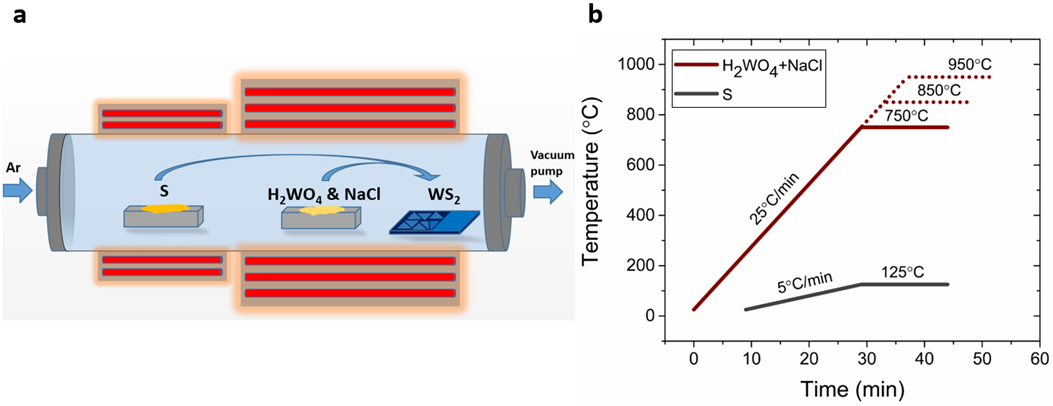
\includegraphics[scale=0.3]{PaperSIFurnace.png}
		\caption{Illustration of: (a) CVD tubular furnace set-up; (b) temperature profile of the sulphur and the W-precursors heaters respectively. The sulphur reaches 125 {\degree}C when the metal precursors are at the maximum temperature. The SiO2/Si wafers used as substrate for WS2 growth are placed 1-8 cm downstream the W-precursors crucible and they are subjected to the same temperature.}
		\label{fig:PaperSIFurnace}
	\end{center}
\end{figure} By following this method a reproducible deposition of large area flakes can be shown. As seen in Figure \ref{fig:PaperOptical} the size of the flakes increases from left to right as the precursors used ($WO_3$, $WO_3-NaCl$ and $H_2WO_4-NaCl$) change as well as demonstrating the lower temperature required to achieve these growths. All of these growths result in formation of triangular flakes with sharp edges and uniformity of colour throughout which suggest a high quality, pristine material across the flake. 
The growth using only $WO_3$ results in formation of small flakes of 10 $\mu m$ at 950 {\degree}C while no growth occurs at lower temperatures (Figure \ref{fig:PaperOptical}. This can be explained by the high sublimation temperature of $WO_3$.

\begin{figure}[h]
\begin{center}
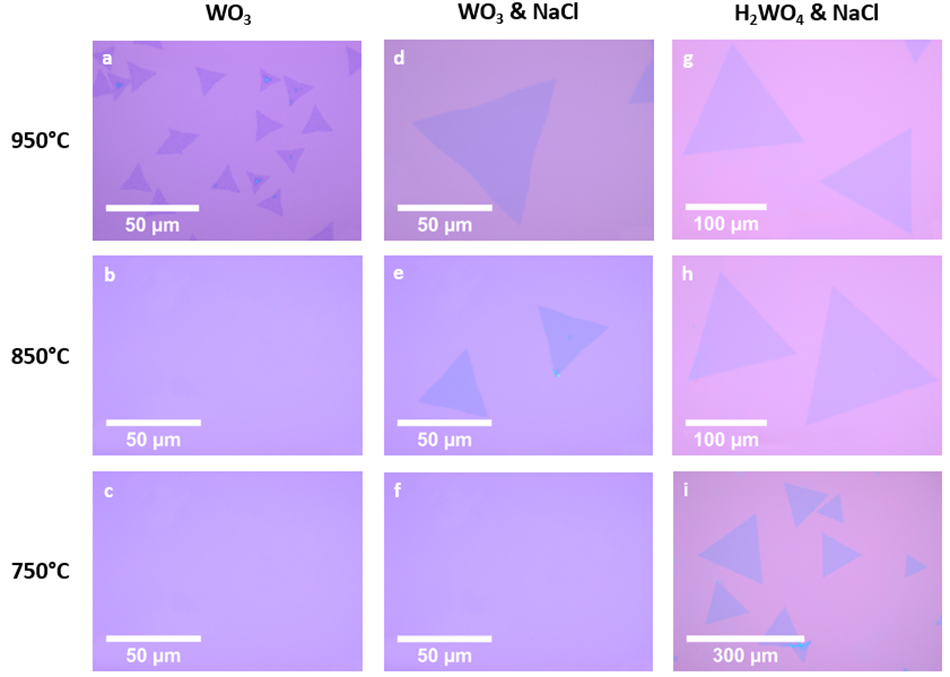
\includegraphics[scale=0.3]{PaperOptical.png}
\caption{Optical micrographs of $WS_2$ triangles grown on $SiO_2/Si$ substrates at different temperatures and using different precursors: (a) $WO_3$ at  950 {\degree}C; (b) $WO_3$ at 850 {\degree}C; (c) $WO_3$ at 750 {\degree}C; (d) $WO_3 + NaCl$ at 950 {\degree}C; (e) $WO_3+NaCl$ at 850 {\degree}C; (f) $WO3 + NaCl$ at 750 {\degree}C, the OM appears as a bare SiO2 substrate; (g) $H_2WO_4 + NaCl$ at 950 {\degree}C; (h) $H_2WO_4 + NaCl$ at 850 {\degree}C; (i) $H_2WO_4 + NaCl$ at 750 {\degree}C.}
\label{fig:PaperOptical}
\end{center}
\end{figure}

The growth can also be observed using $WO_3 + NaCl$ at 950 {\degree}C and 850 {\degree}C with the former showing flakes of size of about 60 $\mu m$ while the latter showing smaller flakes of about 30 $\mu m$ in size. To explain this difference in size a Robinson \& Robin model can be used which states that at higher temperatures the diffusivity of the adsorbed precursors is favourable to the expansion of the existing domains. On the other hand the desorption of the adsorbed species is high leading which limits the supersaturation and formation of new domains. If the temperature is lowered even further to 750 {\degree}C then no growth is observed at all, most likely due to slow evaporation of $WO_3$ precursor. 

With the change of precursors from $WO_3$ to $H_2WO_4$ a signifacnt change in size of flakes is observed at 850 {\degree}C  and higher temperatures with lengths exceeding 200 $\mu m$. Additionally the growth have been shown to occur at 750 {\degree}C with flakes of the size of 50-200 $\mu m$. Moreover continuous monolayer areas of up to 0.8 mm in size has been shown (Figure \ref{fig:PaperSIOpticalContinous}). By increasing the growth pressure (1.6 mbar to 13 mbar) at 950 {\degree}C bilayer $WS_2$ flakes can be preferentially formed (Figure \ref{fig:PaperSIOpticalAFM}.

\begin{figure}[h]
	\begin{center}
		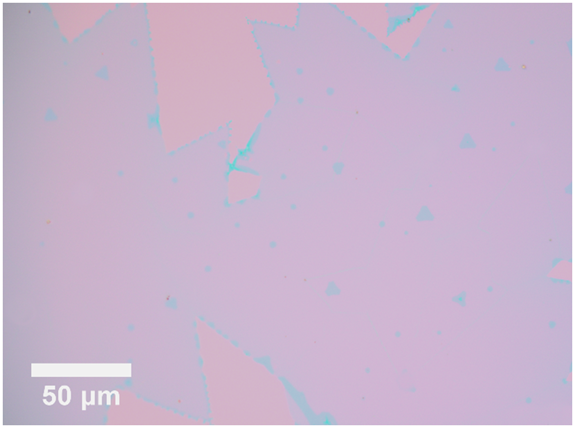
\includegraphics[scale=0.3]{PaperSIOpticalContinous.png}
		\caption{Optical micrograph of continuous layer of $WS_2$}
		\label{fig:PaperSIOpticalContinous}
	\end{center}
\end{figure}

\begin{figure}[h]
	\begin{center}
		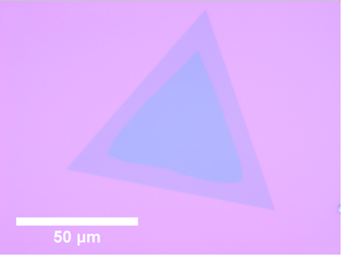
\includegraphics[scale=0.3]{PaperSIOpticalAFM.png}
		\caption{Optical micrograph of $WS_2$ bilayer}
		\label{fig:PaperSIOpticalAFM}
	\end{center}
\end{figure}

%\todo[inline]{Original paper starts here. To be replaced or rewritten}

By replacing WO3 with H2WO4 the lateral size of the WS2 monolayered domains significantly increases (Figure 1g,h,i). The triangular crystals have edge lengths exceeding 200 {$\mu$}m at temperatures higher than 850 {\degree}C and between 50-200 {$\mu$}m at 750 {\degree}C (Figure 1g,h,i). Continuous polycrystalline monolayer coverage has been obtained over areas of {$\sim$}0.8 mm extension (Figure S2). Increasing the growth pressure (from 1.6 mbar to 13 mbar) at 950 {\degree}C bilayered WS2 flakes are preferentially formed (Figure S3). To understand the facilitated synthesis of WS2 using H2WO4 and NaCl, we conducted X-ray diffraction (XRD) analysis of the reaction products between H2WO4+NaCl and WO3+NaCl systems at different temperatures (500 {\degree}C, 650 {\degree}C and 750 {\degree}C) to understand the chemical differences (Figure S4). We found that the main products of the reactions between NaCl and H2WO4 are: NaxWyOz and tungsten oxychloride (WClO4 and WO2Cl2). The NaxWyOz possesses a high evaporation temperature as it remains in the crucible (Figure S5) after the synthesis of WS2 is completed. Further, using this compound as precursors for a new growth of WS2 at 950 {\degree}C did not lead to the formation of any WS2 flakes, confirming the high evaporation temperature. On the bases of previous studies on the synthesis of bulk crystals, the formation of tungsten oxychloride species (WO2Cl2 and/or WOCl4) is likely to occur while the formation of metal halides is less favourable (e.g. WCl6) [ ][ ]. Tungsten oxychlorides are volatile already at 200 {\degree}C [ ] and they can be sulfidized in vapour phase and then be deposited onto the target substrate as atomic clusters. WOCl4 has been previously used [43] as precursor for the CVD synthesis of WS2 bulk films. Despite its strong tungsten oxygen double bonds, WOCl4 proved to be an effective precursor with a clean decomposition pathway in the CVD process without formation of tungsten oxysulfide. We have verified that using this precursor is indeed possible to obtain WS2 at temperatures as low as 550 {\degree}C (Figure S6a). The key role played by the oxyhalide species it becomes apparent if we try to grow WS2 by using only hydrated tungsten oxide. As this decomposes to form WO3, only small WS2 domains are observed with similar PL characteristics to the WO3 precursors-growth (Figure S6b). Furthermore, to confirm the key role played by Cl, we replaced NaCl with KCl and we obtained comparable growth results (Figure S6c).

% paper break

\begin{figure}[h]
	\begin{center}
		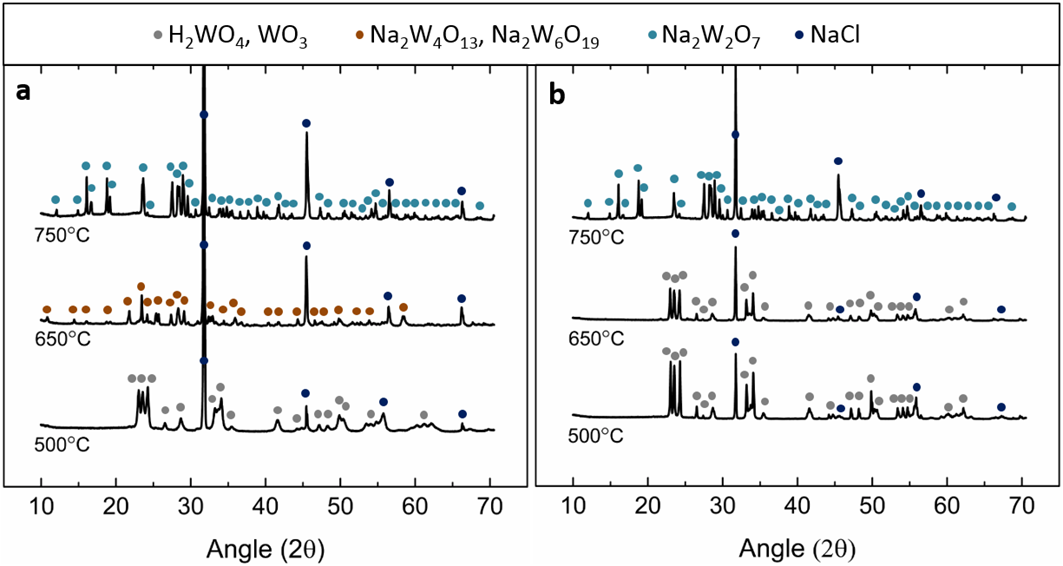
\includegraphics[scale=0.3]{PaperSIXRD.png}
		\caption{XRD pattern of the residual powder of W-precursors after thermal treatment at 500 {\degree}C, 650 {\degree}C and 750 {\degree}C respectivley, using (a) $H_2WO_4+NaCl$ and (b) $WO_3+NaCl$ as precursor.}
		\label{fig:PaperSIXRD}
	\end{center}
\end{figure}

\begin{figure}[h]
		\begin{center}
		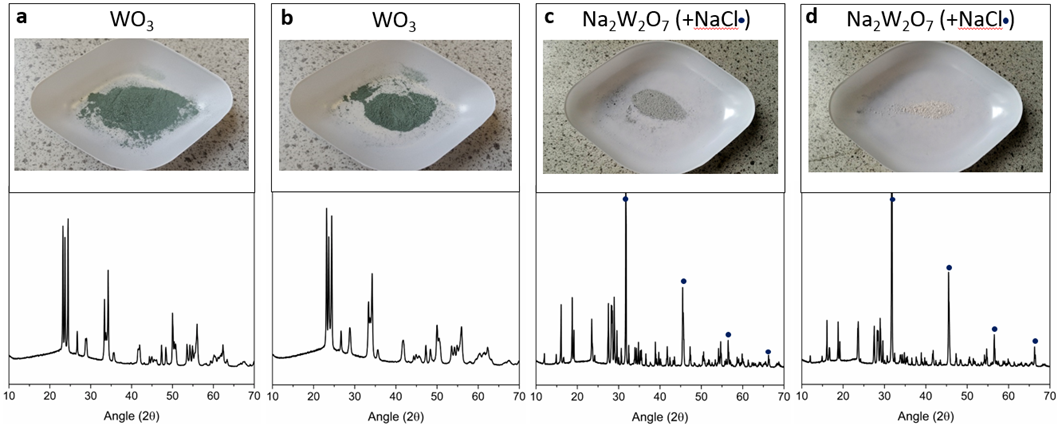
\includegraphics[scale=0.3]{PaperSIXRDOptical.png}
		\caption{Residual powders of the W-precursors and their XRD patterns after thermal treatment at 750{\degree}C using (a) $WO_3$, (b) $H_2WO_4$, (c) $WO_3+NaCl$, and (d) $H_2WO_4+NaCl$ as precursor. The blue dots in the XRD patterns indicate the presence of residual NaCl.}
		\label{fig:PaperSIXRDOptical}
	\end{center}
\end{figure}

The flakes were investigated using HRTEM to confirm high crystallinity of the material (Figure \ref{fig:PaperAFM}. The lattice constant measured in this way has been found to be 0.3 nm, which is consistent with that of 2H-WS2 (0.318 nm). The AFM characterisation allowed to confirm the presence of monolayer (Figure \ref{fig:PaperAFM}) and bilayer (Figure \ref{fig:PaperSIOpticalAFM} flakes with the step of 0.8 nm \cite{Wu2014}\cite{Rasmussen2015}.

The Raman spectroscopy characterisation of $WS_2$ flakes obtained under different growth conditions can be seen in Figure \ref{fig:PaperAFM}. All of these spectra exhibit the main 2 peaks at {$\sim$}(351{$\pm$}0.53) $cm^{−1}$ and {$\sim$}(417.6{$\pm$}1) $cm^{−1}$. The latter peak corresponds to the $A_{1g}$ vibrational mode while the former peak can be further resolved into two peaks, one related to 2LA vibrational mode and the second to $E^1_{2g}$. As seen in the Figure \ref{fig:PaperSIMapsIntensityE} and Figure \ref{fig:PaperSIMapsIntensityA} the distribution of intensity of both main peaks is uniform across the flakes. Similarly the difference between peak positions of $A_{1g}$ and $E^1_{2g}$ is also uniformly distributed as seen in Figure \ref{fig:PaperSIMapsDifference} and is equal to {$\sim$}(66.5{$\pm$}0.53) $cm^{−1}$ which is indicative of monolayer \cite{Withers2014}.

\begin{figure}[h]
\begin{center}
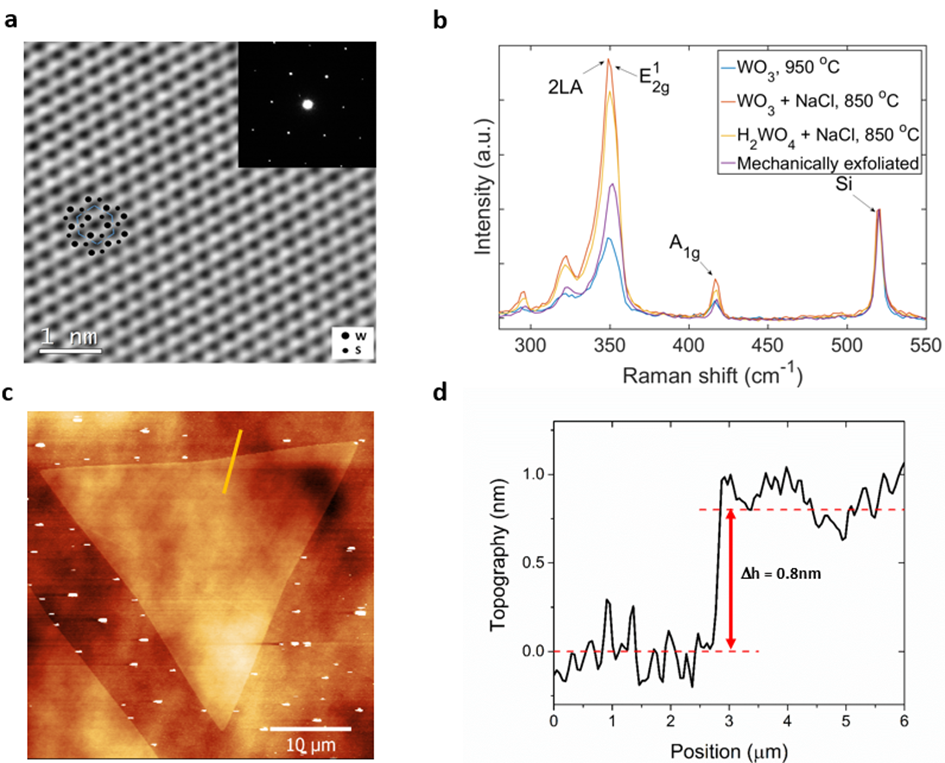
\includegraphics[scale=0.3]{PaperAFM.png}
\caption{Structural and physical characterization of WS2 triangles: (a) HRTEM image of the $WS_2$ lattice grown using $H_2WO_4+NaCl$, the inset report a selected diffraction area which show a hexagonal pattern. (b) Raman spectra showing the characteristics active modes of WS2 grown under different conditions and compared with mechanically exfoliated flakes. (c) AFM image and (d) corresponding thickness profile of monolayer $WS_2$.}
\label{fig:PaperAFM}
\end{center}
\end{figure}

As seen in Figure \ref{fig:PaperPLMaps} maps of PL intensity has been collected for samples grown using different growth condition. The sample grown using $WO_3$ at 950 {\degree}C appears to be trisected into 3 symmetrical areas. The intensity is lowest along the the trisecting lines and highest in the centre of each of the sub-triangles. The PL peak position is inversely proportional to the intensity of the PL peak as seen in Figure \ref{fig:PaperSIMapsPositionPL}. The distribution of the PL peak positions seems to be bimodal with maxima at 1.96 eV and 1.94 eV. The FWHM is distributed mostly uniformly with few small areas of greater and few of smaller FWHM (Figure \ref{fig:PaperSIMapsWidthPL} with the average value of 65 meV. These peak position and FWHM values are comparable with those reported in literature \cite{ExtraordinaryRoomTemperaturePhotoluminescenceInTriangularWS2Monolayers}\cite{Rong2014}\cite{Hu2016}\cite{Kang2015a}. The PL spectra taken from one of the three smaller parts of the flake are redshiftted by about 0.02 eV and are wider than average. This can be explained by the presence of defects, in particular sulfur vacancies, which effectively cause the $WS_2$ to be n-doped \cite{Hui2013}\cite{Peimyoo2014}. This in turn increases the trion population which introduces new peak, redshifted by about 30 meV, which results in overall shift and broadening of the PL peak \cite{Tongay2013}\cite{ExtraordinaryRoomTemperaturePhotoluminescenceInTriangularWS2Monolayers}. Additionally such localised changes in PL peak intensity and position can be caused by local strain \cite{Liu2014}\cite{Hui2013}. To investigate the potential effect of strain on the observed PL pattern a flake was cut using high power 532nm laser. As seen in Figure \ref{fig:PaperSIMapsCutting} the resulting pattern remains the same as before treatment. Therefore the observed pattern is most likely caused by the local variation in defect density \cite{Liu2016}.

By introducing the NaCl and mixing it with $WO_3$ precursor $WS_2$ samples are grown that exhibit higher energy and narrower PL peaks. The spectra are asymetric and can be therefore deconvoluted to obtain an exciton and trion component (Figure \ref{fig:PaperPLSpectraHistograms}). The spatial distribution of the PL position and width is mostly uniform throughout the flake. However the distribution of PL peak positions and FWHM across different flakes grown at the same conditions is bimodal (Figure \ref{fig:PaperPLSpectraHistograms}. The PL peak position is found to be ({$\sim$}1.95{$\pm$}0.002 eV and 1.96{$\pm$}0.002 eV) while the FWHM is ({$\sim$}43{$\pm$}2.8 meV and 51{$\pm$}3 meV) which is smaller than most reported works \cite{ExtraordinaryRoomTemperaturePhotoluminescenceInTriangularWS2Monolayers}\cite{Rong2014}\cite{Hu2016}\cite{Kang2015a}. This can be explained by smaller trion component in the PL spectrum which in turn means that $WS_2$ samples grown at these conditions contain less structural defects compared to the pure $WO_3$ growth. A difference in growth mechanism (topotactic or molecular conversion) which results in different defect distribution can be attributed to the differences in samples.

\begin{figure}[h]
\begin{center}
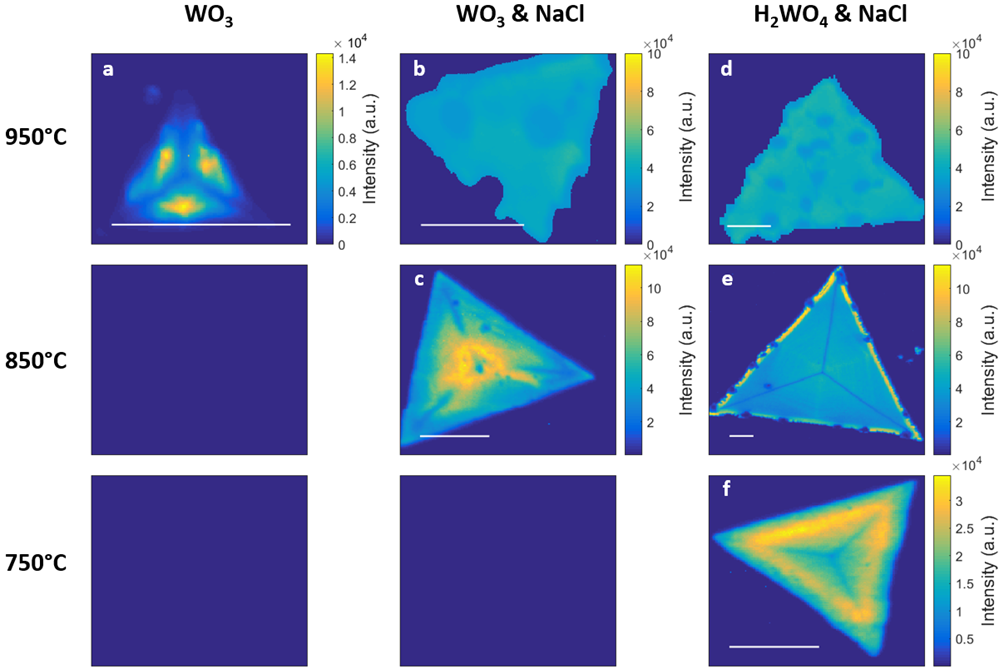
\includegraphics[scale=0.3]{PaperPLMaps.png}
\caption{Spatial maps of PL intensity of $WS_2$ grown in the conditions exemplified in Figure 1. The scale bar length is 10$\mu$m.}
\label{fig:PaperPLMaps}
\end{center}
\end{figure}

By changing the $WO_3$ precursor to the $H_2WO_4$ precursor a further shift in PL peak position, as well as increase in PL intensity and narrowing of he PL peak is observed as seen in Figure \ref{fig:PaperPLMaps}, \ref{fig:PaperPLSpectraHistograms}. The PL peak position distribution across the flake is narrow and is ({$\sim$}1.980{$\pm$}0.005 eV) which is higher than that of the $WO_3$ and $WO_3 + NaCl$ systems. The FWHM is found to be ({$\sim$}36{$\pm$}3 meV) which is also smaller than that of the $WO_3$ and $WO_3 + NaCl$ systems. The PL peak width is also smaller than that reported in literature for CVD grown \cite{ExtraordinaryRoomTemperaturePhotoluminescenceInTriangularWS2Monolayers}\cite{Rong2014}\cite{Hu2016}\cite{Kang2015a} exfoliated $WS_2$ \cite{EvolutionOfElectronicStructureInAtomicallyThinSheetsOfWS2AndWSe2}\cite{doi:10.1021/nn5059908}. At the same time it is comparable to the $WS_2$ grown on van der Waals substrates \cite{doi:10.1021/nn503093k} as well as mechanically exfoliated $WS_2$ \cite{doi:10.1021/nl500171v}. Additionally the peak position as well as FWHM variation is also smaller than that of other samples (5meV and 3 meV respectively) (Figure \ref{fig:PaperSIScatterComparison}. The PL peak intensity map (Figure \ref{fig:PaperPLMaps}) shows that the spatial distribution of intensity is also much more homogeneous with faint weak pattern of three trisecting lines still visible.

\begin{figure}[h]
\begin{center}
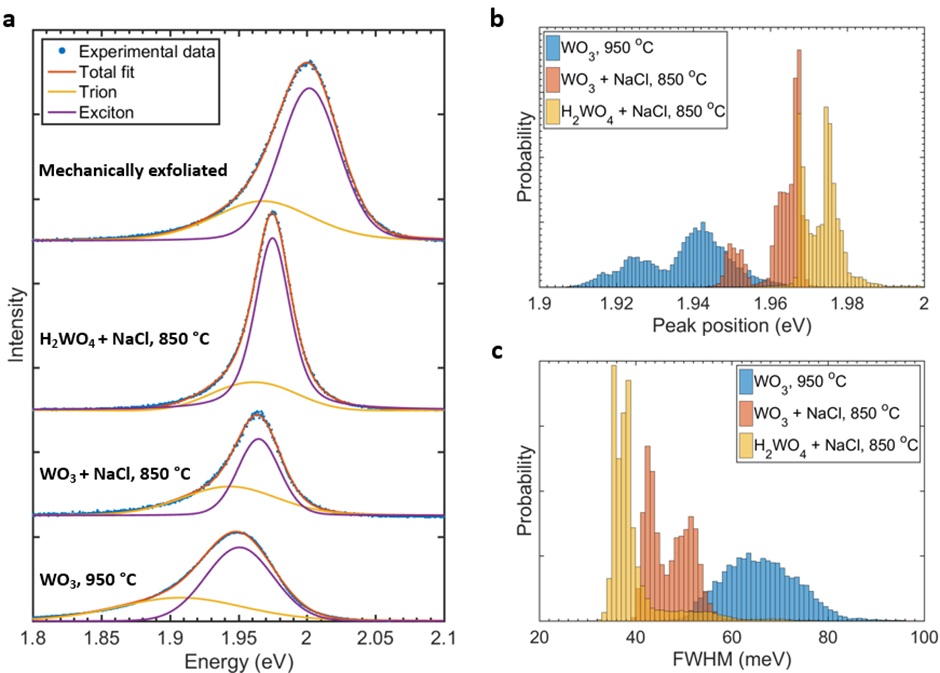
\includegraphics[scale=0.3]{PaperPLSpectraHistograms.png}
\caption{PL spectra characteristics of $WS_2$ grown using: $WO_3$ at 950 {\degree}C, $WO_3+NaCl$ at 850 {\degree}C, $H_2WO_4+NaCl$ at 850 {\degree}C: (a) individual spectra (dotted line) and deconvolution in exciton and trion components; (b) distribution of PL peak position and (c) distribution of PL FWHM for several $WS_2$ grown using the three different precursor systems.}
\label{fig:PaperPLSpectraHistograms}
\end{center}
\end{figure}

As seen in Figure \ref{fig:PaperSIMapsRaman} the Raman peaks are generally uniform in both intensity and position for most samples. The irregularities in the intensity and position of both the $E^1_{2g}$ and $A_{1g}$ in the sample grown at 950 {\degree}C with both $WO_3 + NaCl$ and $H_2WO_4 + NaCl$ are caused primarily by residue deposited on top of the flakes after the growth as seen in optical micrographs. Additionally as seen in Figure \ref{fig:PaperSIMapsIntensityE} the deviations from the mean value are located primarily at the edges of the sample. This suggests that the rest of flake is pristine and the deviations are associated with residue located at the edges. The coefficient of variation (CV) for the intensity and position for the samples grown at 950 {\degree}C with $WO_3$ and at 850 {\degree}C with $WO_3 + NaCl$ and $H_2WO_4 + NaCl$ is on the order of up to $10^{-4}$ which indicates a very high homogenity across the samples. This further shows that the crystal quality of the flakes is quite uniform regardless of the growth method.

\begin{figure}[h]
	\begin{center}
		\begin{subfigure}[b]{0.4\textwidth}
			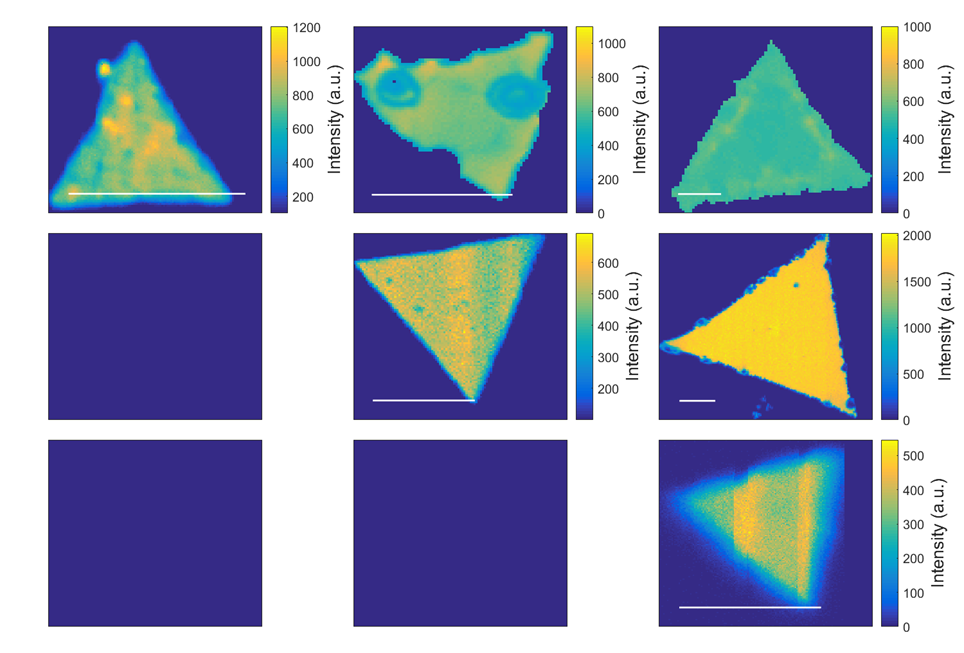
\includegraphics[width=\textwidth]{PaperSIMapsIntensityE.png}
			\caption{Maps of Raman $E^1_{2g}$ peak intensity}
			\label{fig:PaperSIMapsIntensityE}
		\end{subfigure}
		\quad
		\begin{subfigure}[b]{0.4\textwidth}
			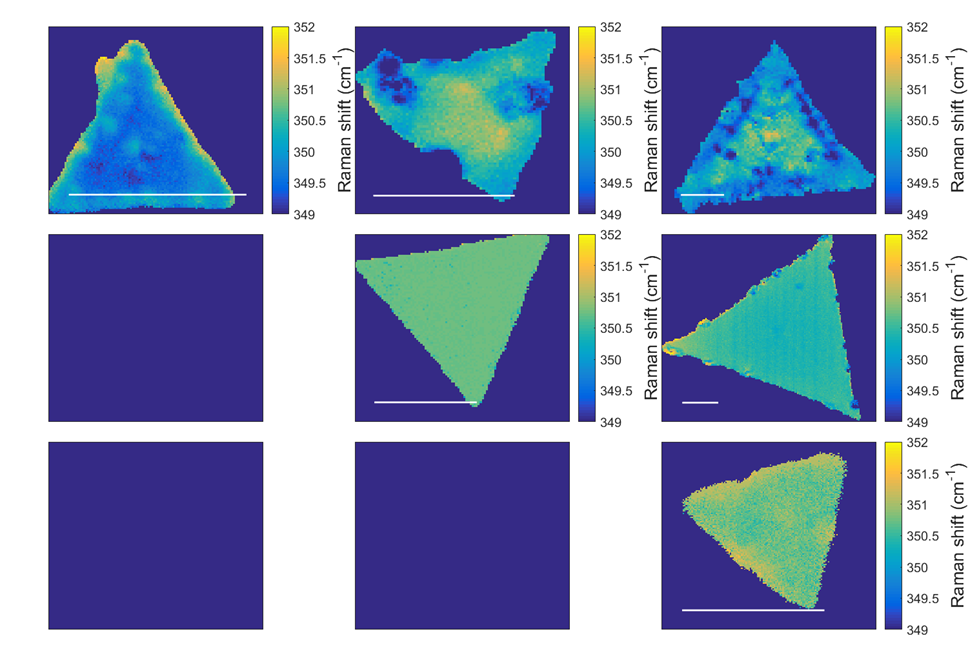
\includegraphics[width=\textwidth]{PaperSIMapsPositionE.png}
			\caption{Maps of Raman $E^1_{2g}$ peak position}
			\label{fig:PaperSIMapsPositionE}
		\end{subfigure}
		\hfill
		\begin{subfigure}[b]{0.4\textwidth}
			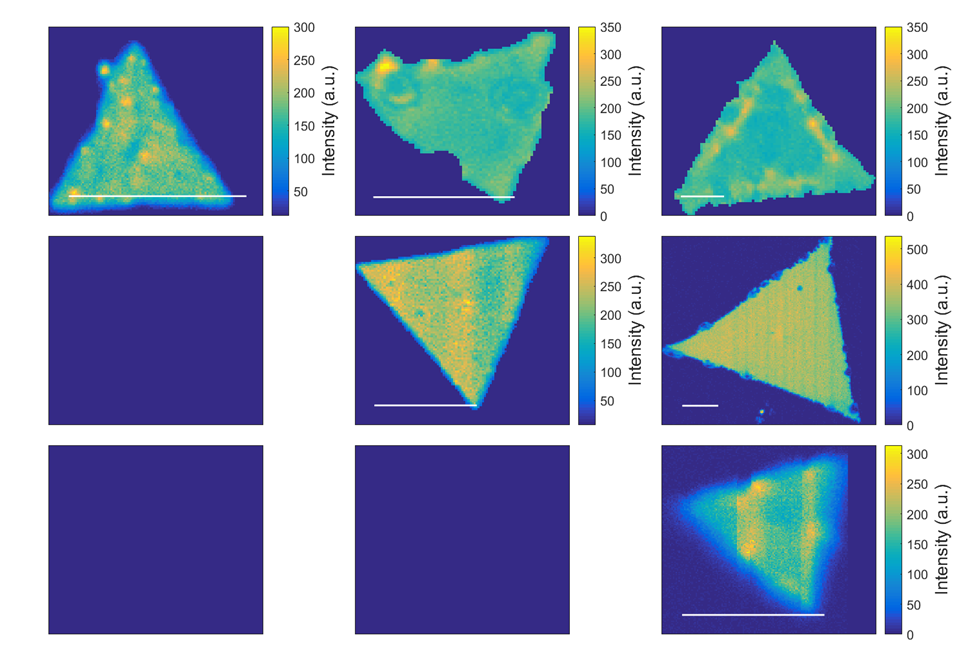
\includegraphics[width=\textwidth]{PaperSIMapsIntensityA.png}
			\caption{Maps of Raman $A_{1g}$ peak intensity}
			\label{fig:PaperSIMapsIntensityA}
		\end{subfigure}
		\quad
		\begin{subfigure}[b]{0.4\textwidth}
			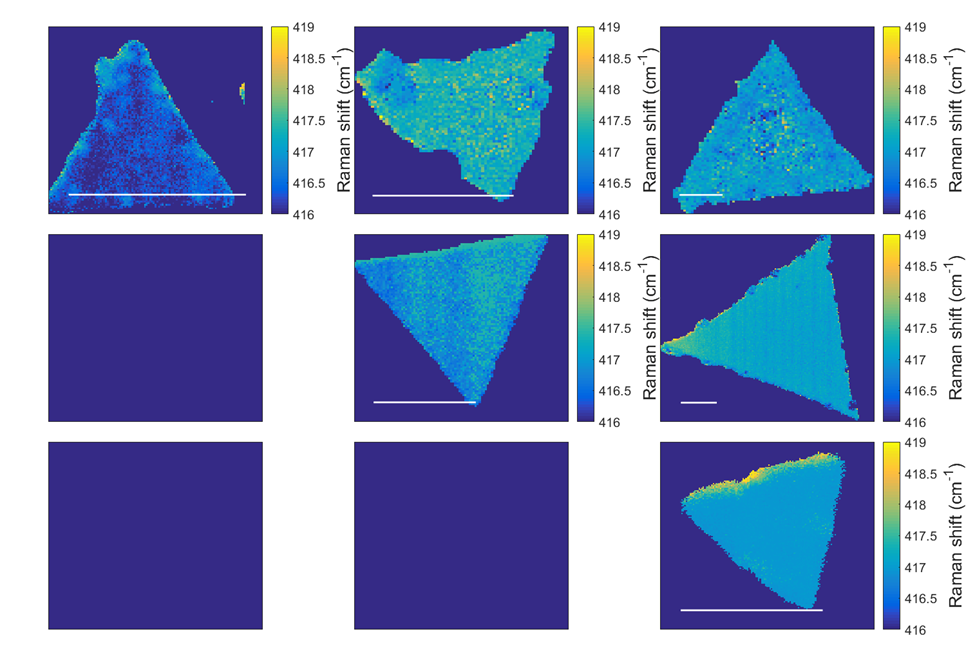
\includegraphics[width=\textwidth]{PaperSIMapsPositionA.png}
			\caption{Maps of Raman $A_{1g}$ peak position}
			\label{fig:PaperSIMapsPositionA}
		\end{subfigure}
		\caption{Maps of Raman peaks intensities and positions}
		\label{fig:PaperSIMapsRaman}
	\end{center}
\end{figure}

By looking at the difference in position between $A_{1g}$ and $E^1_{2g}$ peak positions as seen in Figure \ref{fig:PaperSIMapsDifference} is can be further concluded that the flakes are uniformly monolayer. The deviations from the mean are heavily localised and correlated with differences in PL as well as optical images and are most likely caused by precursors residue. Additionally no trisecting lines (as seen in Figure \ref{fig:PaperPLMaps}) can be seen in the maps of Raman spectra.

\begin{figure}[h]
	\begin{center}
		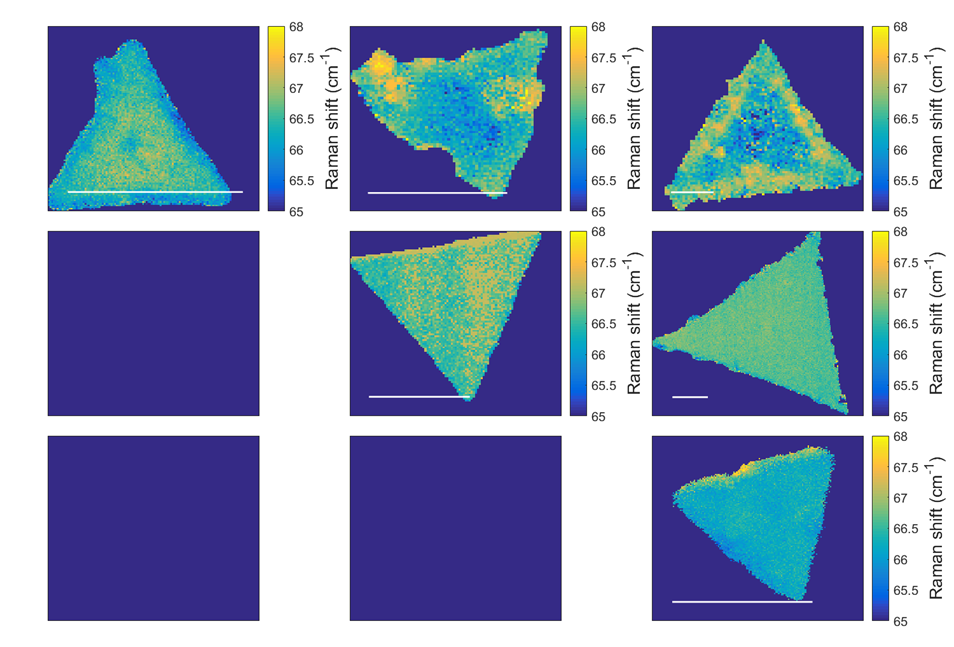
\includegraphics[scale=0.3]{PaperSIMapsDifference.png}
		\caption{Raman spectroscopy: $2LA-A_{1g}$ energy differences. Scale bar is 10 $\mu$m}
		\label{fig:PaperSIMapsDifference}
	\end{center}
\end{figure}

The maps of PL peak positions and widths can be seen in Figure \ref{fig:PaperSIMapsPL}. The PL positions map of the sample grown at 950 {\degree}C using $WO_3$ shows some variability with spots of lower energy that loosely correlate with the PL intensity. There is still faintly visible pattern of three trisecting lines of higher energy as seen in Figure \ref{fig:PaperPLMaps}. This indicates the areas with higher intensity correlate with lower peak position, especially along the trisecting lines. The other maps, especially the ones grown at 850 {\degree}C and 750 {\degree}C with $WO_3 + NaCl$ and $H_2WO_4 + NaCl$, are more uniform in terms of PL peak position and PL peak width. The deviations are again highly localised and correlated with the deviations in Raman and PL intensity. These deviations are generally of lower PL peak position as well as greater PL peak width which generally indicates lower crystal quality.

\begin{figure}[h]
	\begin{center}
		\begin{subfigure}[b]{0.4\textwidth}
			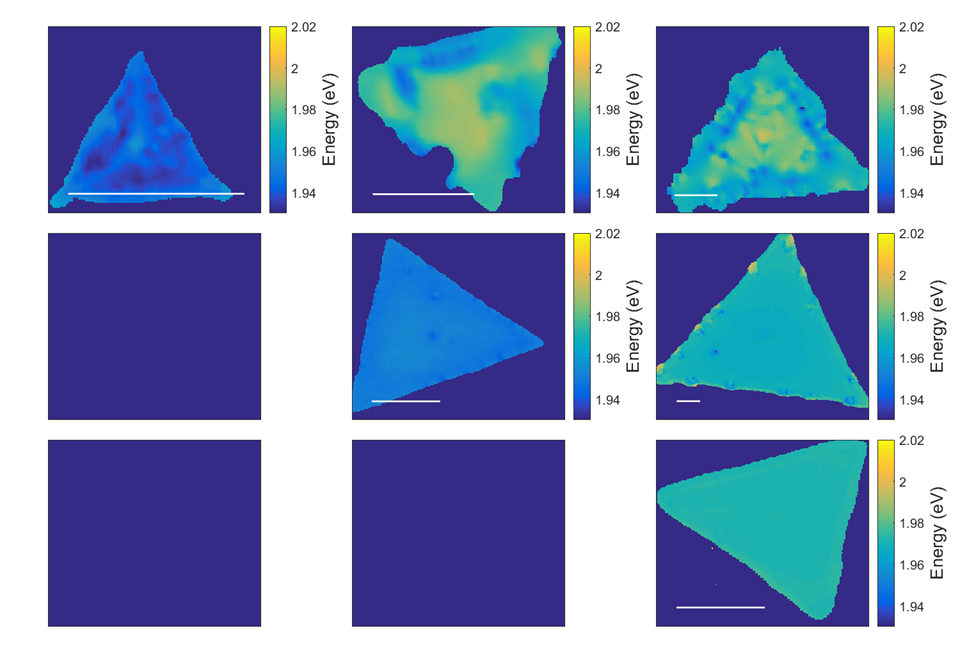
\includegraphics[width=\textwidth]{PaperSIMapsPositionPL.png}
			\caption{Maps of PL peak position}
			\label{fig:PaperSIMapsPositionPL}
		\end{subfigure}
		\quad
		\begin{subfigure}[b]{0.4\textwidth}
			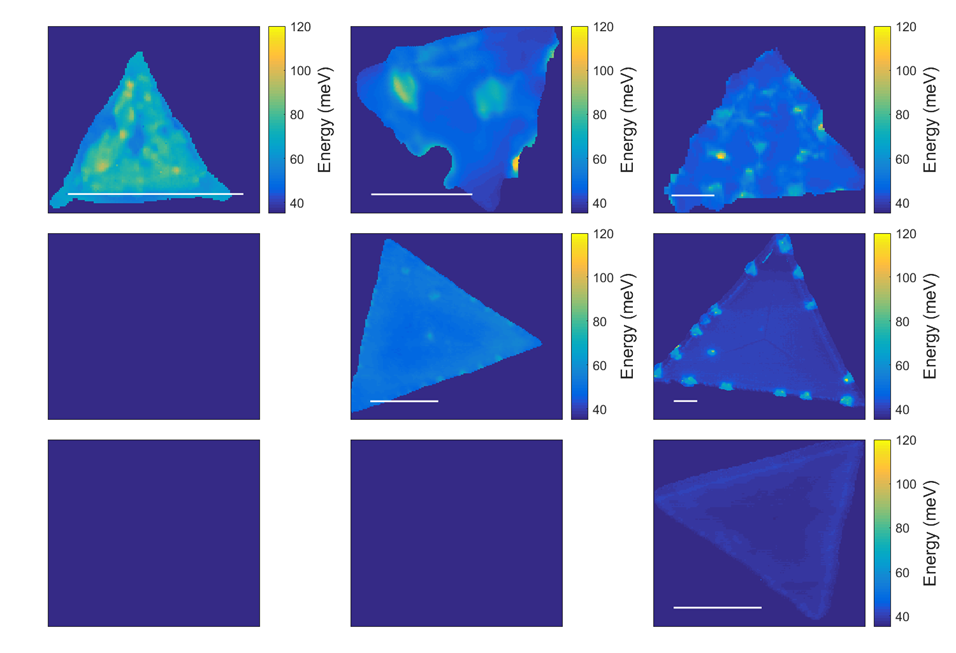
\includegraphics[width=\textwidth]{PaperSIMapsWidthPL.png}
			\caption{Maps of PL peak width}
			\label{fig:PaperSIMapsWidthPL}
		\end{subfigure}
		\caption{Maps of PL peak positions and width}
		\label{fig:PaperSIMapsPL}
	\end{center}
\end{figure}

One possible explanation of the pattern of trisecting lines as seen in e.g. Figure \ref{fig:PaperPLMaps} is the thermal strain caused by difference in thermal expansion coefficient between $WS_2$ and the $SiO_2$ substrate. Since it is known that the strain in TMDCs including $WS_2$ can casue the change in Raman and PL spectrum \cite{Liu2014}\cite{Hui2013} then removing a piece of the material should cause the strain to adapt to new bounding conditions. In order to investigate the trisecting pattern a flake with such pattern has been cut using 532 nm high intensity laser (50 mW). As seen in Figure \ref{fig:PaperSIMapsCutting} both the PL intensity maps and Raman $E^1_{2g}$ maps show a clear separation. The resulting PL and Raman intensity maps however do not show any significant change in the pattern. The trisecting lines as well as local maxima can still be seen in PL intensity map. The Raman shows few spots of increased intensity on of the halves of the flake as well as a very weak increased intensity area along the cut. Since there is no observed increased intensity along any edges before cutting the flake it does not appear that the increased intensity along the cut is a result of strain being resolved into new bounding conditions. It appears therefore that cutting the material did not alter the pattern nor alter the rest of the PL or Raman spectra maps.

\begin{figure}[h]
	\begin{center}
		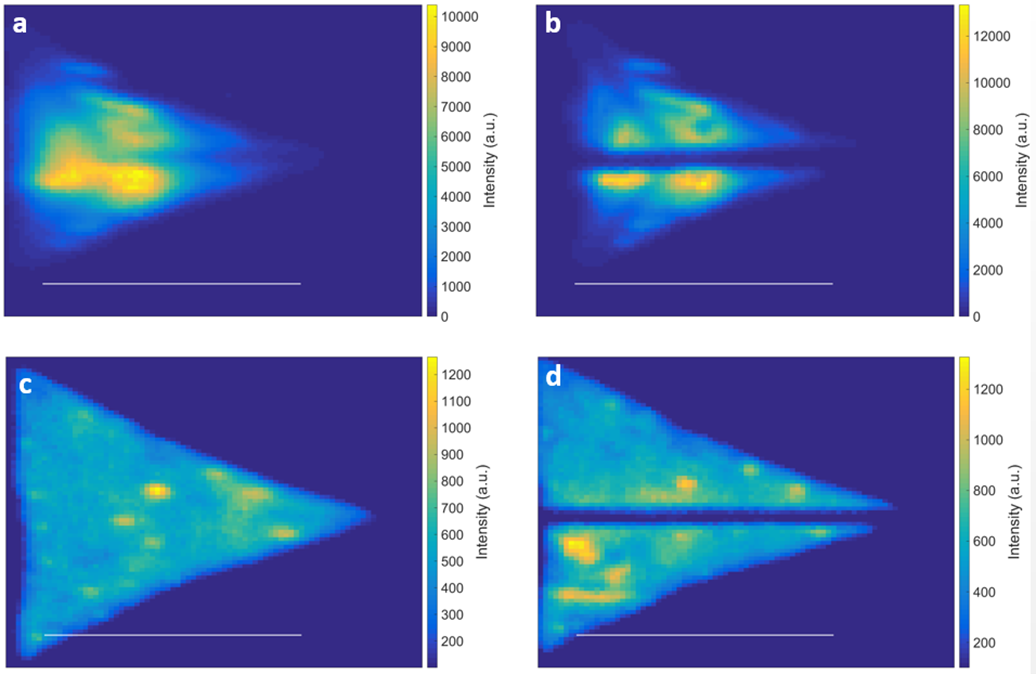
\includegraphics[scale=0.3]{PaperSIMapsCutting.png}
		\caption{PL intensity (a) before and (b) after the cutting. $2LA+E^1_{2g}$ Raman intensity (c) before and (d) after the cutting. Scale bar is 10 $\mu$m}
		\label{fig:PaperSIMapsCutting}
	\end{center}
\end{figure}

The spectral maps from different flakes grown with the same conditions were then collected and plotted as graphs of intensity or width versus position. As seen in Figure \ref{fig:PaperSIScatterComparison} the PL intensity seems to be largely independent of the PL position. If PL is present at given position then intensity is mostly uniformly distributed in terms of intensity. The PL width seems to be inversely related with regards to PL position. In samples grown at 850 {\degree}C with $WO_3 + NaCl$ the relation seems to be the strongest. Across all the samples the values vary between around 60-80 meV at low PL energies (1.92 eV) to 40-60 meV at high PL energies (1.98 eV). This seems to be related to overall quality of the crystals, i.e. the presence of defects, stoichiometry, crystallinity, doping, adatoms. The more uniform the sample the less mechanisms for peak broadening as well as fewer added energy levels facilitating different electron recombination paths.

\begin{figure}[!h]
	\begin{center}
		\begin{subfigure}[b]{0.8\textwidth}
			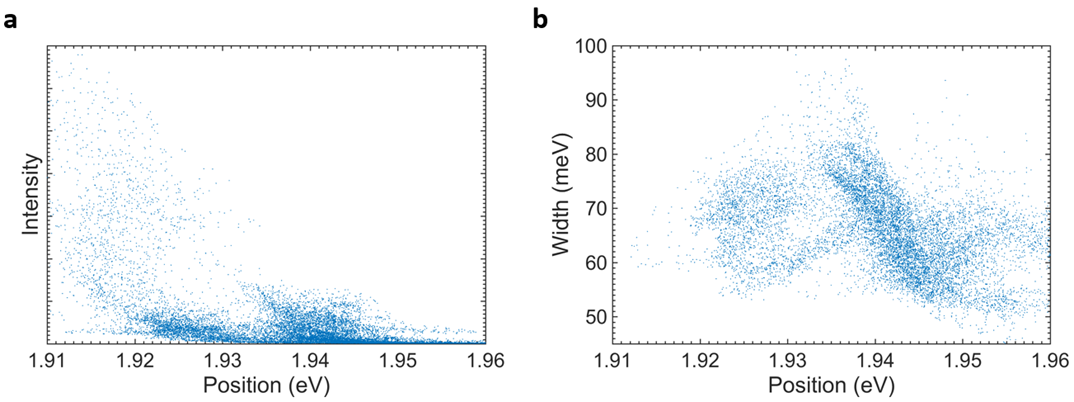
\includegraphics[scale=0.3]{PaperSIScatterWO3.png}
			\caption{(a) PL Intensity vs position, (b) PL FWHM vs position of $WS_2$ grown using $WO_3$ at 950 {\degree}C}
			\label{fig:PaperSIScatterWO3}
		\end{subfigure}

		\begin{subfigure}[b]{0.8\textwidth}
			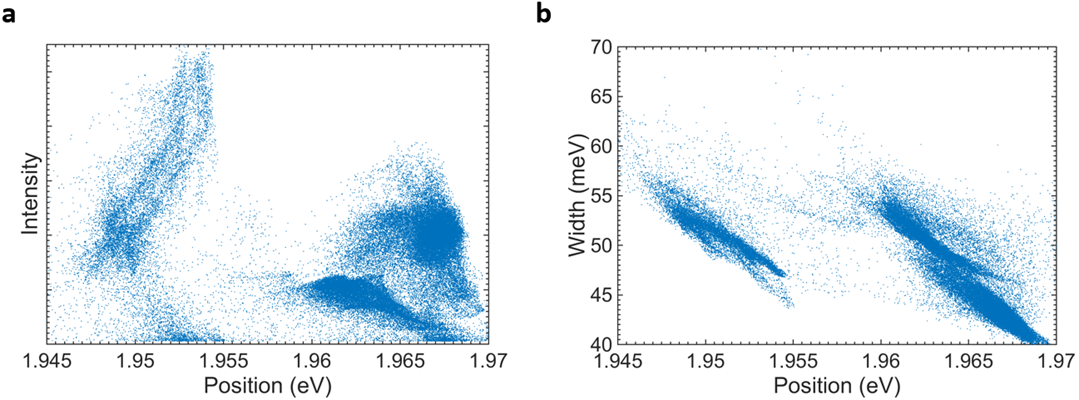
\includegraphics[scale=0.3]{PaperSIScatterWO3NaCl.png}
			\caption{PL Intensity vs position, (b) PL FWHM vs position of $WS_2$ grown using $WO_3+NaCl$ at 850 {\degree}C}
			\label{fig:PaperSIScatterWO3NaCl}
		\end{subfigure}

		\begin{subfigure}[b]{0.8\textwidth}
			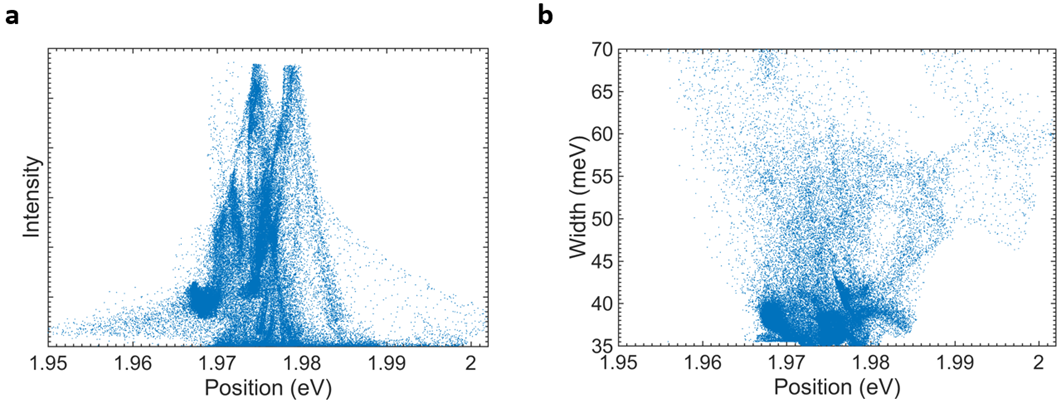
\includegraphics[scale=0.3]{PaperSIScatterH2WO4NaCl.png}
			\caption{(a) PL Intensity vs position, (b) PL FWHM vs position of $WS_2$ grown using $H_2WO_4+NaCl$ at 850 {\degree}C}
			\label{fig:PaperSIScatterH2WO4NaCl}
		\end{subfigure}

		\begin{subfigure}[b]{0.8\textwidth}
			\includegraphics[scale=0.3]{PaperSIScatterComparison.png}
			\caption{(a) PL Intensity vs position, (b) PL FWHM vs position of $WS_2$ grown using $WO_3$, $WO_3+NaCl$, $H_2WO_4+NaCl$}
			\label{fig:PaperSIScatterComparison}
		\end{subfigure}
	\end{center}
\end{figure}

The chemical composition of the flakes grown using $H_2WO_4 + NaCl$ has been investigated using XPS. The W 4f5/2 and W 4f7/2 core levels show peak positions that of the $W^{4+}$ in $WS_2$ \cite{Cattelan2015}\cite{Martinez2004} (32.7 eV 34.8 eV respectively) with FWHM of 1 eV (Figure \ref{fig:PaperXPS}, the smallest possible using Mg K$\alpha$ x-ray source. It means therefore that the $WS_2$ is of perfect stoichiometric ratio of W and S. Additionally by integrating the intensity of the W 4f and S 2p core level peaks the same result is achieved. Furthermore the S 2p1/2 and 2p3/2 core levels are also present at the expected position for $WS_2$ (162.3 eV and 163.4 eV respectively, Figure \ref{fig:PaperXPS}) and small FWHM of 1 eV \cite{Martinez2004}. Small peaks indicative of $W^{6+}$ (W 4f5/2 and W 4f7/2 at 35.9 eV and 38.1 eV respectively, Figure \ref{fig:PaperXPS}) can be attributed to presence of $WO_3$ and which partially overlaps with W 5p core level (38.5 eV). These peaks however disappear after the flakes are transferred to another $Si/SiO_2$ substrate, suggesting that they can be caused by residue $WO_3$ given that the XPS spot size is relatively big ({$\sim$}1 mm). The FWHM of the W 4f core levels was unchanged after the transfer, indicating that the crystallinity and the quality of the flakes was preserved with no extra defects introduced.

The $WS_2$ samples grown using $WO_3 + NaCl$ have been characterised by XPS as well and the stoichiometric ratio of 2:1 for S:W has been found. However the $W^{6+}$ component, caused most likely by presence of $WO_3$ (W 4f5/2 and W 4f7/2 at 35.9 eV and 38.1 eV respectively) is more pronounced indicating incomplete sulfurisation. Similarly to the sample grown with $H_2WO_4 + NaCl$ this component disappears entirely upon transferring the sample onto new $Si/SiO_2$ indicating it is present around the flakes, distributed across the substrate. The $W^{4+}$ 4f core levels peak width is {$\sim$}1.2 eV which indicates higher defect concentration compared to that of the sample grown using $H_2WO_4 + NaCl$. This FWHM however increases after the transfer, which is most likely caused by the increase in the concentration of the defects caused by the mechanical stress during the transfer. In conclusion the $H_2WO_4$ is shown to be a better precursor compared to $WO_3$.
 
\begin{figure}[h]
\begin{center}
\includegraphics[scale=0.3]{PaperXPS.png}
\caption{XPS spectra of the W 4f and S 2p core level peak regions. (a) Comparison  of W 4f5/2 , W 4f7/2  and W 5p core levels of WS2 grown using H2WO4+NaCl at 950 {\degree}C (blue spectrum) with WS2 grown using WO3+NaCl at 950 {\degree}C (red spectrum). The deconvolution of W 4f5/2 , W 4f7/2  and W 5p core levels and overall fit of the spectrum are reported as black dashed and a continuous line respectively. (b) The S 2p1/2 and 2p3/2 core levels for each of the two growth conditions are reported in the central panel. (c) W 4f5/2 , W 4f7/2  and W 5p core levels before (dashed line) and after transfer (continuous like) onto a new SiO2/Si substrate are compared showing the complete disappearance of the residual WO3 components. The spectra were fit by Doniach-Sunjic function after subtracting a Shirley background (black dashed line).}
\label{fig:PaperXPS}
\end{center}
\end{figure}

The samples were further characterised for their electrical properties. Bottom-gated field effect transistors were prepared as seen in Figure \ref{fig:PaperElectricalMeasurementMonolayer}. The FET transfer curve indicates accumulation-type n-channel transistor, where the drain current increases with applied gate bias after a threshold is crossed. Once the current-bias curve reaches linear range it can be described by $I_d = {\mu}_nC_{ox}(W/L) ((V_{gs}-V_{th})V_{ds})$, where ${\mu}_n$ is the electron field-effect mobility, $C_ox$ is the oxide dielectric and $V_th$ is the threshold voltage. As seen in Figure \ref{fig:PaperElectricalMeasurementMonolayer} a typical response curve for both the as grown as well as transferred samples of $WS_2$ grown with $H_2WO_4$ show an asymmetry around $V_{ds}=0$ V due to difference in the source and drain potentials. The Schottky barrier at the source is pinned by the gate, while the barrier at the drain diminishes proportionally to the drain bias and vice versa. The contacts however become more "Ohmic", when the bands bend more at the semiconductor/metal interface while the gate bias increase, leading to more significant tunnelling current.

\begin{figure}[h]
\begin{center}
\includegraphics[scale=0.3]{PaperElectricalMeasurementMonolayer.png}
\caption{Electrical characteristics of monolayer WS2: (a) Schematic of the bottom-gated field effect transistors; (b) optical micrograph of the device (scale bar is 20${\mu}$m); (c) FET transfer curve for the monolayer WS2 grown using H2WO4+NaCl at 950 {\degree}C showing the highest mobility of 28 cm2/Vs (linear region of the transport graph marked with a red-dashed line); (d) Response curves at different gate biases for a WS2 triangle grown using H2WO4+NaCl; (e) FET transfer curve for the monolayer WS2 grown using WO3+NaCl at 800 {\degree}C; (f) electron mobilities of monolayer WS2 grown using different conditions.}
\label{fig:PaperElectricalMeasurementMonolayer}
\end{center}
\end{figure}

By looking at the linear regime of the transport graph (red-dashed line in Figure \ref{fig:PaperElectricalMeasurementMonolayer}) the field-effect mobility can be calculated as ${\mu}_n=C_{ox}^{-1}(d{\sigma}/dV_{gs})$. The electron mobility calculated for $WS_2$ grown with $H_2WO_4 + NaCl$ is generally higher than that of $WS_2$ grown with $WO_3 + NaCl$ (Figure \ref{fig:PaperElectricalMeasurementMonolayer}) which further indicates higher crystal quality when using $H_2WO_4$. The monolayer $WS_2$ exhibits electron mobility of 28 $cm^2 V^{-1} s^{-1}$, the highest reported value for CVD grown $WS_2$ and transferred onto $SiO_2$ \cite{Li2015}\cite{Kang2015}\cite{Gao2015}\cite{doi:10.1021/nn403454e}\cite{doi:10.1021/acsnano.5b01480}\cite{Lee2013}\cite{Yun2015}\cite{Alharbi2016}\cite{Lan2015}\cite{Hussain2013}\cite{Cui2015} and comparable to mechanically exfoliated $WS_2$ \cite{Withers2014}\cite{Iqbal2016}\cite{Georgiou2014}\cite{Iqbal2015a}. The highest mobilities were recorded in $WS_2$ grown at 950 {\degree}C, grown with either $H_2WO_4 + NaCl$ or $WO_3 + NaCl$, which indicates a role of the growth temperature in improving the quality of the $WS_2$. As the temperature is lowered the difference between precursors becomes more pronounced in terms of the crystal quality. The $H_2WO_4 + NaCl$ precursor system grown $WS_2$ shows electron mobility of 10 to 20 $cm^2 V^{-1} s^{-1}$ at temperatures of 750 {\degree}C and 850 {\degree}C. The electron mobilities of $WS_2$ grown using $WO_3 + NaCl$ are much lower, {$\sim$}2 $cm^2 V^{-1} s^{-1}$ at 800 $\sim$C. Bilayer $WS_2$ samples have overall greater electron mobility than their monolayer equivalent (between {$\sim$}38 $cm^2 V^{-1} s^{-1}$ and 52 $cm^2 V^{-1} s^{-1}$), similarly to the mechanically exfoliated flakes \cite{Ovchinnikov2014}\cite{Iqbal2015a}. The electron mobility of bilayer $WS_2$ (52 $cm^2 V^{-1} s^{-1}$) (Figure \ref{fig:PaperElectricalMeasurementBilayer} and Figure \ref{fig:PaperMobilityComparison}) is also higher than that of other CVD grown $WS_2$ as well as mechanically exfoliated onto $SiO_2$ samples of $WS_2$ reported  \cite{Iqbal2015}\cite{Ovchinnikov2014}\cite{Iqbal2015a}. The highest mobility has been obtained for bilayer system using $WO_3 + NaCl$ indicating that the precursor choice is less important for electron mobility in such systems. 

\begin{figure}[h]
\begin{center}
\includegraphics[scale=0.3]{PaperMobilityComparison.png}
\caption{Comparison of our results with the literature of CVD grown material and mechanically exfoliated WS2 (MEX) : electron mobility for (a) monolayer WS2 and (b) bilayer WS2. The histograms show our record values for both monolayer and bilayer amongst the best values reported for CVD grown WS2.}
\label{fig:PaperMobilityComparison}
\end{center}
\end{figure}
 
\begin{figure}[h]
\begin{center}
\includegraphics[scale=0.3]{PaperElectricalMeasurementBilayer.png}
\caption{Electrical characteristics of bilayer WS2: (a) Optical micrograph of the device (scale bar is 30$\mu$m); (b) FET transfer curve for the bilayer WS2 grown using WO3+NaCl at 950 {\degree}C showing the highest mobility of 52 cm2/Vs (linear region of the transport graph marked with a red-dashed line); (c) electron mobility of bilayer WS2 grown by using different precursor systems.}
\label{fig:PaperElectricalMeasurementBilayer}
\end{center}
\end{figure}

\section{Conclusions}

In conclusion a synthesis route has been developed that allows for high quality monolayer and bilayer $WS_2$ CVD growth. This quality is demonstrated by highest recorded electron FET mobility for both monolayer and bilayer CVD grown $WS_2$ compared to the literature and comparable to that of mechanically exfoliated ones. Additionally the triangle flakes grown using $H_2WO_4 + NaCl$ are much larger (up to {$\sim$200-300 $\mu m$) compared to ones grown using standard $WO_3$. The CVD growth using $H_2WO_4$ has also been demonstrated to work at lower temperatures, down to 750 {\degree}C compared to more commonly used 950 {\degree}C. Finally the PL of the $WS_2$ grown using $H_2WO_4$ is is uniform throughout the flake and has very FWHM (36 meV) which again points to high crystal quality and lack of defects in form of sulfur vacancies. These findings allow to develop further the TMDCs synthesis method of CVD and can potentially lead to industrially scalable synthesis of monolayer $WS_2$ or other TMDCs over large area.
%\chapter{Low T PL}

\section{Introduction}

As the temperature of the semiconductor goes down the number of charge carriers decreases. Because of this in $WS_2$ the number of electrons is expected to be lower at low temperatures. Additionally as the temperature drops the peak broadening due to temperature effects i.e. Gaussian broadening decreases. At room temperature the thermal energy is equal to about 25 meV which limits the smallest possible width of the peak and therefore the resolution. Both of those effects should result in the peak at low temperatures to be overall weaker and more narrow than that at the room temperature. Additionally the lower electron density should result in lower population of trions. Due to lower temperature the electron and hole mobility should also decrease and cause the excitons to be more often trapped at defects sites also known as bound excitons.

\section{Experimental}

In order to perform the low temperature measurement the sample was placed in an environmental stage, Linkam THMS350V. The stage allows the sample to be cooled down to the temperatures of liquid nitrogen ($LN_2$) and at pressures of down to $10^{-3}$ mbar. The stage was then placed in a Renishaw Raman spectroscope chamber and the spectra were collected using 532nm green laser.

\section{Results}

The PL measurements were taken from the $WS_2$ monolayer on $Si/SiO_2$ sample at different conditions. As seen in Figure \ref{fig:LowTPLComparison} the PL from has been measured in the same spot at lower pressure ($2 \times 10^{-2}$) and different temperatures, room temperature and liquid nitrogen ($LN_2$) temperature ($-196 \degree C$). The PL from that spot at room temperature is centred at 1.957 eV and has FWHM of 44.3 meV. After lowering the temperature to that of $LN_2$ i.e. $-196 \degree C$ the PL measurement was taken again and the intensity of the peak was found to be about 0.81 that of the RT. Additionally the position of the PL at lower temperature was found to be 1.969 eV and the FWHM was 37.9 eV.

\begin{figure}[!ht]
	\begin{center}
		\includegraphics[scale=0.4]{LowT/LowTPLComparison.png}
		\caption{PL spectra of samples at room temperature and $LN_2$ temperature at $2 \times 10^{-2}$ mbar}
		\label{fig:LowTPLComparison}
	\end{center}
\end{figure}

The PL spectra were then fitted with 2 peaks to resolve the trions and excitons. The results can be seen in Figure \ref{fig:LowTPLDeconvolution}. Similarly the PL spectrum from room temperature has been fitted with two peaks. The intensity ratio between the exciton and trion in the low temperature sample is about 4, while at the room temperature it is 3. The FWHM of the exciton peak also lowers from 36 meV to about 32 meV.

This indicates that indeed as the temperature is lowered the FWHM of the PL peak and especially the exciton component also lowers. However the difference between the FWHM at room temperature and low temperature is not as big as expected if temperature was the main contributor to the peak broadening. For room temperature a thermal energy contribution should be about 25 meV while at $LN_2$ temperature (77 K) the contribution should be about half of that, i.e. 12 meV. The peak was fitted mostly with Gaussian lineshape (about 70\%) and therefore the temperature should be a significant contributor to the peak width. It is possible that the laser heats up the sample during measurement since the thermal contact between the substrate and the cooled stage is weak. Additionally the glass window separating the stage and the room environment as well as the substrate itself can be covered in water droplets which could introduce refraction and therefore peak broadening.  

\begin{figure}[!ht]
	\begin{center}
		\includegraphics[scale=0.4]{LowT/LowTPLDeconvolution.png}
		\caption{PL spectra at low temperature with trions and excitons components resolved}
		\label{fig:LowTPLDeconvolution}
	\end{center}
\end{figure}

Due to the low FWHM of the PL peaks a strong trion component can be observed as seen in Figure \ref{fig:LowTPLStrongTrion}. While the lower temperature of the substrate can explain the small FWHM, the trion component is much stronger than in standard measurement environment. This could be caused by the low pressure which results in less oxygen and water molecules adsorbed at the defect sites. At standard conditions (1 atm) these species adsorb at the defect sites and attract electrons which as a result lowers the overall n-doping level of the material. 

\begin{figure}[!ht]
	\begin{center}
		\includegraphics[scale=0.4]{LowT/LowTPLStrongTrion.png}
		\caption{Low temperature PL spectrum with easily resolved strong trion component}
		\label{fig:LowTPLStrongTrion}
	\end{center}
\end{figure}

In order to check the influence of the pressure on the PL and potential effect of the adsorbed oxygen, nitrogen and water molecules measurement at different pressures was conducted. As seen in Figure \ref{fig:LowTPLPressureDifference} as the pressure is lowered by several orders of magnitude the PL peak is shifted to the red. The FWHM of the PL peak at the ambient pressure is about 41 meV while at lower pressure ($1.5 \times 10^{-2}$ mbar) it is about 44 meV. The exciton to trion intensity ratio changes from 3.387 to 3.25 from the ambient pressure to low pressure. It therefore indicates that as the pressure is lowered the trion component becomes more prominent and the peak overall shifts to lower energies. 

\begin{figure}[!ht]
	\begin{center}
		\includegraphics[scale=0.4]{LowT/LowTPLPressureDifference.png}
		\caption{PL measurements at different atmospheric pressures}
		\label{fig:LowTPLPressureDifference}
	\end{center}
\end{figure}


\chapter{Transfer}
\label{cha:Transfer}
\section{Introduction}
		The most common method of producing the TMDCs is CVD. During the CVD growth the process the substrate and the sample are heated to very high temperatures, up to 1000 {\degree}C. Because of that there is substantial thermal expansion in both substrate and sample. However due to difference in thermal expansion coefficient between those two elements there is potential build up of thermal strain. Additionally because the substrate, upon which the sample is grown, is heated to such high temperatures that it cannot be used for electrical measurements. More specifically the thermal expansion coefficients of $WS_2$ and $SiO_2$ are on the order of $10^{-3}$ and $10^{-7}$ $K^{-1}$ respectively \cite{Hu2018}\cite{Tada2000}. Therefore it is expected that during cooling down the $WS_2$ will come under tension due to thermal expansion coefficient misalignment. Moreover in order to use TMDCs as components in devices different layers have to arranged together either vertically or laterally. Due to aforementioned reasons there is a need to develop methods for transferring single layers of TDMCs from one substrate to another one. In this chapter a focus is put on transferring $WS_2$ monolayer flakes from $SiO_2/Si$ onto other surfaces.
		
\section{Experimental}
		
	The most common method of transferring flakes synthesised via CVD method is a wet transfer method utilising as an intermediate substrate. In such procedure a thin layer of PMMA is first spun on top of the substrate. After drying the substrate is placed in a KOH aqueous solution (6\% to 8\%) heated to about 50 {\degree}C. As a result the thin layer of $SiO_2$ on top of $Si$ is dissolved leaving a PMMA with the sample attached to it floating on top of the solution. The PMMA is then rinsed in water several times and scooped up onto a new substrate. Next the sample is dried and annealed to ensure good adhesion and remove wrinkles and strain. Then the PMMA is removed with a solution of acetone and IPA at about 50 {\degree}C. Any remaining PMMA can be removed by annealing the sample at about 100 {\degree}C.  
		
\section{Results}
	
	A sample has been investigated using Raman and PL spectroscopy before and after transfer. In Figure \ref{fig:TransferPLMapsComparison} a comparison between samples before and after transfer can be seen in PL spectra. The as grown sample shows mostly homogeneous PL intensity, position and FWHM across the sample with the exception of the edge and trisecting lines in the middle where the PL intensity is higher and lower accordingly. In the sample after transfer the PL intensity, position and FWHM is more randomly distributed across the flake and there is a distinct lack of edge enhancement or the presence of trisecting lines.
	
	The position of the PL peak from the as grown sample is $1.9765 \pm (9.8445 \times 10^{-4})$ eV, while the PL peak position from transferred sample $1.9703 \pm (8.3518 \times 10^{-3})$ eV. Therefore the peak position is shifted by 6.2 meV after transfer while the relative standard deviation is about 8.5 times greater in the transferred sample than in the as grown sample. The FWHM in the as grown sample is $36.3693 \pm 0.7982$ meV while in the transferred sample the FWHM is $83.2706 \pm 6.7947$ meV. The FWHM then increases by 46.9013 meV while the relative standard deviation increases 3.726 times compared to the as grown sample.

	The Raman $E^1_{2g}$ peak position in the as grown sample is $350.8681 \pm 0.2064$ $cm^{-1}$ while in the transferred sample is $351.3407 \pm 0.2893$ $cm^{-1}$. The relative uncertainty is therefore 1.3997 greater in the transferred sample. The position of the Raman $A_{1g}$ peak in the as grown sample is $418.6530 \pm 0.2829$ $cm^{-1}$ while in the transferred sample it is $417.3195 \pm 0.4760$ $cm^{-1}$ . The relative uncertainty is therefore $1.6879$ times greater in the transferred sample. The position difference between these two peaks is $67.7862 \pm 0.2411$ $cm^{-1}$ in the as grown sample while it is $66.0040 \pm 0.4757$ $cm^{-1}$ in the transferred sample. The relative uncertainty increases therefore by $2.0264$ after the transfer. The intensity ratio between those peaks in the as grown sample is $5.7471 \pm 0.6844$ and after transfer it is $7.1609 \pm 0.8899$. The relative uncertainty changes $1.5835$ times after transfer.
	
	It can be therefore seen that after transfer the relative uncertainty increases for every parameter of Raman and PL spectra maps. This indicates that the sample after the transfer is much less homogeneous. Because both the position of PL as well as the position of Raman peaks is affected by the strain the inhomogeneity can indicate a relaxation or build up of strain. Since the CVD growth method involves heating up the sample and the substrate to very high temperatures, up to $850 {\degree}C$, there is possibility of residual thermal strain after cooling down. Since the PMMA is much more flexible than the $SiO_2$, that the sample is grown on, the $WS_2$ can relax before being placed on a new $SiO_2$ substrate. On the other hand the water present in between the $WS_2$ and PMMA can also be a source of strain. During the water evaporation the surface tension can induce local strain leading to high inhomogeneity. The PMMA can also have varying thickness and can swell to small degree therefore contracting in size during drying. Any or all of these effects can potentially contribute to the variation in parameters observed.
	
	The average values of peak fitting parameters can be then compared between the two sample states to estimate the strain in the sample. The average position of $E^1_{2g} + 2LA$ peak changes from 350.8601 $cm^{-1}$ to 351.3407 $cm^{-1}$, a 0.4806 $cm^{-1}$ difference. Since the position of this peak changes by -3.1 $cm^{-1} / \%$ this indicates the change in strain of -0.155$\%$. The $E^1_{2g} + 2LA$ peak intensity change ($\Delta I / I_0$) of 23.15$\%$ indicates a 0.23$\%$ change in strain. The average value of $A_{1g}$ peak position changes from 418.6530 $cm^{-1}$ to 417.3195 $cm^{-1}$, a difference of 1.3335 $cm^{-1}$. This indicates then a strain of -4.445$\%$. The intensity change of $A_{1g}$ peak of 25.64$\%$ corresponds to 0.3344$\%$ strain.
	
	The PL peak position changes from 1.9765 eV to 1.9703 which corresponds to change from about 1$\%$ to 0.75$\%$ strain, a -0.25$\%$ change.
	
	By comparing different average Raman and PL peaks fit parameters it is not clear to what extent the $WS_2$ is strained before or after the transfer. Neither the direction nor the extent of strain can be estimated then in the sample overall. The difference in deviation of theses values however indicates that the sample after transfer is less homogeneous than before. Therefore while it cannot be said that the sample strain changes on average as a whole, there is a change in strain across the sample. While the thermal strain should result in the sample as a whole being under tension due to thermal expansion and contraction other effects could still take place like aforementioned variation in water presence, inhomogeneity of PMMA layer thickness or folds in PMMA layer.
	
\begin{figure}[ht] %PL Transfer Maps
	\begin{center}
		\begin{subfigure}[b]{0.4\textwidth}
			\includegraphics[scale=0.15]{Transfer/TransferPLIntensityMapAsgrown.png}
			\caption{PL Intensity map of as grown sample}
			\label{fig:TransferPLIntensityMapAsgrown}
		\end{subfigure}
		\quad
		\begin{subfigure}[b]{0.4\textwidth}
			\includegraphics[scale=0.15]{Transfer/TransferPLIntensityMapTransferred.png}
			\caption{PL Intensity map of transferred sample}
			\label{fig:TransferPLIntensityMapTransferred}
		\end{subfigure}
		\vfill
		\begin{subfigure}[b]{0.4\textwidth}
			\includegraphics[scale=0.15]{Transfer/TransferPLPositionMapAsgrown.png}
			\caption{PL Position map of as grown sample}
			\label{fig:TransferPLPositionMapAsgrown}
		\end{subfigure}
		\quad
		\begin{subfigure}[b]{0.4\textwidth}
			\includegraphics[scale=0.15]{Transfer/TransferPLPositionMapTransferred.png}
			\caption{PL Position map of transferred sample}
			\label{fig:TransferPLPositionMapTransferred}
		\end{subfigure}
		\vfill
		\begin{subfigure}[b]{0.4\textwidth}
			\includegraphics[scale=0.15]{Transfer/TransferPLWidthMapAsgrown.png}
			\caption{PL FWHM map of as grown sample}
			\label{fig:TransferPLWidthMapAsgrown}
		\end{subfigure}
		\quad
		\begin{subfigure}[b]{0.4\textwidth}
			\includegraphics[scale=0.15]{Transfer/TransferPLWidthMapTransferred.png}
			\caption{PL FWHM map of transferred sample}
		\label{fig:TransferPLWidthMapTransferred}
		\end{subfigure}
		\caption{PL spectra maps of samples before and after transfer}
		\label{fig:TransferPLMapsComparison}
	\end{center}
\end{figure}
	
\begin{figure}[ht] %Raman Transfer Maps
	\begin{center}
		\begin{subfigure}[b]{0.4\textwidth}
			\includegraphics[scale=0.15]{Transfer/TransferRamanIntensityEMapAsgrown.png}
			\caption{Raman $E^1_{2g}$ intensity map of as grown sample}
			\label{fig:TransferRamanIntensityEMapAsgrown}
		\end{subfigure}
		\quad
		\begin{subfigure}[b]{0.4\textwidth}
			\includegraphics[scale=0.15]{Transfer/TransferRamanIntensityEMapTransferred.png}
			\caption{Raman $E^1_{2g}$ intensity map of transferred sample}
			\label{fig:TransferRamanIntensityMapTransferred}
		\end{subfigure}
		\vfill
		\begin{subfigure}[b]{0.4\textwidth}
			\includegraphics[scale=0.15]{Transfer/TransferRamanIntensityAMapAsgrown.png}
			\caption{Raman $A_{1g}$ intensity map of as grown sample}
			\label{fig:TransferRamanIntensityAMapAsgrown}
		\end{subfigure}
		\quad
		\begin{subfigure}[b]{0.4\textwidth}
			\includegraphics[scale=0.15]{Transfer/TransferRamanIntensityAMapTransferred.png}
			\caption{Raman $A_{1g}$ intensity map of transferred sample}
			\label{fig:TransferRamanIntensityAMapTransferred}
		\end{subfigure}
		\vfill
		\begin{subfigure}[b]{0.4\textwidth}
			\includegraphics[scale=0.15]{Transfer/TransferRamanPositionEMapAsgrown.png}
			\caption{Raman $E^1_{2g}$ position map of as grown sample}
			\label{fig:TransferRamanPositionEMapAsgrown}
		\end{subfigure}
		\quad
		\begin{subfigure}[b]{0.4\textwidth}
			\includegraphics[scale=0.15]{Transfer/TransferRamanPositionEMapTransferred.png}
			\caption{Raman $E^1_{2g}$ position map of transferred sample}
			\label{fig:TransferRamanPositionEMapTransferred}
		\end{subfigure}
		\caption{Raman spectra maps of samples before and after transfer}
		\label{fig:TransferRamanMapsComparison}
	\end{center}
\end{figure}
	
\begin{figure}[ht] %Raman Difference and Ratio Transfer Maps
	\begin{center}
		\begin{subfigure}[b]{0.4\textwidth}
			\includegraphics[scale=0.15]{Transfer/TransferRamanDiffMapAsgrown.png}
			\caption{Raman peak position difference map of as grown sample}
			\label{fig:TransferRamanDiffMapAsgrown}
		\end{subfigure}
		\quad
		\begin{subfigure}[b]{0.4\textwidth}
			\includegraphics[scale=0.15]{Transfer/TransferRamanDiffMapTransferred.png}
			\caption{Raman peak position difference map of transferred sample}
			\label{fig:TransferRamanDiffMapTransferred}
		\end{subfigure}
		\vfill
		\begin{subfigure}[b]{0.4\textwidth}
			\includegraphics[scale=0.15]{Transfer/TransferRamanRatioMapAsgrown.png}
			\caption{Raman peaks ratio map of as grown sample}
			\label{fig:TransferRamanRatioAMapAsgrown}
		\end{subfigure}
		\quad
		\begin{subfigure}[b]{0.4\textwidth}
			\includegraphics[scale=0.15]{Transfer/TransferRamanRatioMapTransferred.png}
			\caption{Raman peaks ratio map of transferred sample}
			\label{fig:TransferRamanRatioAMapTransferred}
		\end{subfigure}
		\caption{Raman spectra maps of samples before and after transfer}
		\label{fig:TransferRamanDiffRatioMapsComparison}
	\end{center}
\end{figure}
	
\section{Conclusions}
	
In this Chapter we have presented the transfer methodology that we have developed in our own way for monolayer TMDCs. Overall the quality of the transfer material is good and the flakes are pristine in shape. It is unclear to what extent the CVD grown $WS_2$ sample is strained prior to transfer or after it. The difference in relative uncertainty of different fitting parameters of PL and Raman spectra however reveals that the sample becomes less homogeneous following the procedure. This could indicate that a certain degree of strain is introduced as a result of the transfer. This in turn could be attributed to the presence of a non uniform distribution of water molecules, non uniform thickness of PMMA layer, folds in the PMMA layer or presence of residue PMMA.
\chapter{Post-transition metal doping of monolayer $WS_2$}

\section{Introduction}

Single layer TMDC materials present a range of unique optical, electrical and mechanical properties which make them promising materials beyond graphene in future nanotechnologies. Atomic doping can further extend the potential of TMDCs since it has been predicted that a number of properties can be tuned trough compositional variation. Up until now doping has relied on charge transfer induced by changing the environmental conditions such as surface adsorption, metal contacts and dielectric interfaces. This approach has demonstrated to severely limit the device working conditions thus doping trough stable incorporation of non-volatile metal atoms is highly preferred. Achieving controlled doping is a challenge which is aggravated by the fact that established synthesis protocols for these materials are still lacking.

Doping of monolayer $WS_2$ with post-transition metals has not been reported as yet. Doping of $WS_2$ with post-transition metals can lead to chemisorbed intercalated atoms between layers which can be regarded as analogous to deep level impurities. It can lead to an additional energy level near to the top of the valence band or, alternatively, as a modification of the energy band of the host crystal due to the interaction between the intercalate and W or S atoms \cite{Yacobi1979}\cite{Yacobi1979a}. In particular indium may generate an additional energy state at the top of the valence band which leads to a subsequent upward shift of this band \cite{Deshpande2001}. A gradual increase in this shift with increasing number of intercalating atoms would lead to a linear decrease in the energy gap with increasing In content as observed in In-intercalated bulk $WS_2$ \cite{Deshpande2001}. This led to the demonstration of higher conductivity and photocurrent than both pure $WS_2$ films thus proving to be highly photo-active. Unlike their alkali and alkaline earth metal analogues, In-intercalated bulk $WS_2$ compounds were found to be stable against oxidation when exposed to air or chemical due to a fairly strong guest-host bonding which hinders deintercalation processes and preserving a perfect 2H crystalline phase \cite{Deshpande2001}\cite{Rao1981}. Further, In has lower melting and boiling points than B, Al and Ga enabling doping via CVD or MOCVD synthesis of $WS_2$ at low temperatures. These characteristics make Indium a very interesting prospected dopant of $WS_2$ to pave the way towards applications as photoelectrodes in solar cells. Post transition metals are prone to intercalate between the layers however displaying very different effect with respect to the alkali and alkaline earth metal intercalates of $WS_2$.

Here we demonstrate indium doping of monolayer $WS_2$ in–situ during CVD synthesis of $WS_2$. The process relies on the addition of a volatile indium precursor which results in large-area In-doped $WS_2$ atomic layers exhibiting tunable optical properties and a semiconducting-to-metallic transition at high doping levels. We also demonstrate controlled indium content from 0 up to 45\% in $WS_2$ maintaining a 2D morphology and atomically thin nature of the material without sacrificing the lateral extension and scalability of the synthesis process.

\section{Results}

The In doped $WS_2$ samples were grown by following the synthesis route developed for the monolayer $WS_2$ as discussed in Chapter \ref{cha:WS2} \cite{Reale2017}. The main change was to add $In(OH)_3$ powder as an indium precursor to the same crucible as W precursor. Such mixed powders in a crucible were then placed in the centre of the furnace similarly to the established procedure.

A first indication of the effect of indium in the $WS_2$ is provided by the morphology of the triangular domains. SEM and OM images of $WS_2$ domains grown by using different $In(OH)_3/H_2WO_4$ weight ratios [$In_{0.25}WS_2$, $In_{0.5}WS_2$, $In_{0.75}WS_2$, $In_1WS_2$] are shown in Figure \ref{fig:InOMSEMImages}. While from the optical contrast it is possible to see that the monolayer nature of the domains is unchanged, it can be noticed how the shape of triangles progressively change. Triangles with straight edges similar to that of pristine $WS_2$ are displayed for low In content while convex and jagged edges appear by increasing the Indium content, which might suggest a more significant incorporation of the latter. $WS_2$ with high indium content can also present different morphologies and even large coverage.

\begin{figure}[!ht]
	\begin{center}
		\begin{subfigure}[b]{0.7\textwidth}
			\includegraphics[width=\textwidth]{In/OMSEMImages1.png}
			\label{fig:InOMSEMImages1}
		\end{subfigure}
		\qquad
		\begin{subfigure}[b]{0.7\textwidth}
			\includegraphics[width=\textwidth]{In/OMSEMImages1.png}
			\label{fig:InOMSEMImages2}
		\end{subfigure}
		\caption{OM and SEM images of flakes grown with different $In(OH)_3/H_2WO_4$ weight ratios: (a, b) 0.25, (c, d) 0.5, (e, f) 0.75 and (g, h)=1.}
		\label{fig:InOMSEMImages}
	\end{center}
\end{figure}

The samples were further characterised using XPS to assess the exact chemical content and therefore the level of doping.

\begin{figure}[!h]
	\begin{center}
		\begin{subfigure}[b]{0.6\textwidth}
			\includegraphics[width=\textwidth]{In/XPSW4f.png}
			\caption{W 4f}
			\label{fig:InXPSW4f}
		\end{subfigure}
		\qquad
		\begin{subfigure}[b]{0.6\textwidth}
			\includegraphics[width=\textwidth]{In/XPSS2p.png}
			\caption{S 2p}
			\label{fig:InXPSS2p}
		\end{subfigure}
		\begin{subfigure}[b]{0.6\textwidth}
			\includegraphics[width=\textwidth]{In/XPSIn3d.png}
			\caption{In 3d}
			\label{fig:InXPSIn3d}
		\end{subfigure}
		\caption{XPS spectra comparison}
		\label{fig:InXPSSpectra}
	\end{center}
\end{figure}

Figure \ref{fig:InXPSSpectra} shows the In 3d, W 4f and S 2p core levels XPS spectra for pure $WS_2$ and In-doped $WS_2$ (In/W=0.25, In/W=0.5, In/W=1). It is immediately noticable that the the sample with 0.25:1 In:W precursor ratio does not exhibits any In 3d peak. At the same time the samples with 0.5:1 In:W as well as 1:1 In:W show pronounced In 3d5/2 core level peak at 445.8 eV and 446.0 eV respectively and In 3d3/2 at 453.3 eV and 453.8 eV respectively. This slight shift might be attributed to the presence of $In_xW_yS_z$ compounds \cite{Wagner1991}. The In 3d core levels for 1:1 In:W sample are also about twice as intense as the ones for the 0.5:1 In:W sample. Furthermore the W 4f core levels for the 1:1 In:W sample are significantly shifted to the blue which might indicate presence of $W^{6+}$ in the doped sample compared to $W^{4+}$ to pure $WS_2$. This would indicate bonding between W and In atoms. The S 2p1/2 and S 2p3/2 core levels for 0.25:1 In:W ratio can be observed at 162.9 eV and 164.1 eV respectively while for the 0.5:1 In:W sample they are at 163.4 eV and 164.6 eV respectively. No to very weak peak can be observed for the 1:1 In:W ratio sample. There is therefore indication of interaction between the S and In atoms, with stronger S 2p core level peak shifts than those of the W 4f core levels. It is therefore possible that the In atoms became chemisorped on the surface, intercalated in between the layers or incorporated as an interstitial. The stoichiometric composition was then calculated using the concentrations of elements from peak integration of In 3d, W 4f and S 2p core levels as seen in Table \ref{tab:InRatios}.

\begin{table}[!ht]
\caption{In:W and S:W ratios obtained by calculating the In, W and S concentrations from the integrated intensity of the In3d, W4f and S2p core levels.}
\label{tab:InRatios}
\end{table}

\begin{center}
\begin{tabular}{c|cc}

Sample 		& In/W 		& S/W\\\hline
In/W = 0.25 & 0.038:1 	& 2.32:1\\
In/W = 0.5	& 0.45:1	& 2.22:1\\
In/W = 1	& 1.98:1	& 0.27:1

\end{tabular}
\end{center}

The XRD diffraction patterns of all the In-doped $WS_2$ samples can all be indexed on a hexagonal unit cell basis (Figure \ref{fig:InXRDAll}) and an analogy can drawn to the pattern of $2H-WS_2$. The most intense reflection is the (002) and for pure and In-doped $WS_2$ (Figure \ref{fig:InXRDIn}) it can be seen that the FWHM decreases as the In precursor concentration increases and that a peak shift towards a larger d spacing (Table \ref{tab:InXRDData}) occurs for the highest indium content. Additionally the samples with indium content of In/W=0.5, In/W=0.75 and In/W=1 show an additional reflection at $2{\Theta}=13.44$ not belonging to $WS_2$, which can be an indicator of successful incorporation of In atoms.

\begin{table}[!ht]
\caption{Data for the (002) XRD peak and lattice parameters for pure $WS_2$ and In-doped $WS_2$ samples.}
\label{tab:InXRDData}
\end{table}

\begin{center}
\begin{tabular}{c|ccccc}

Sample 		& Position (2$\Theta$)	& FWHM (2$\Theta$)	& a (\r{A})	& c (\r{A})	& d (\r{A})	\\\hline
$WS_2$	 	& 14.44 				& 0.703				& 3.23		& 11.02		& 5.51		\\
In/W = 0.25	& 14.47					& 0.294				& 3.23		& 11		& 5.50		\\
In/W = 0.5	& 14.444				& 0.168				& 3.22		& 11.02		& 5.51		\\
In/W = 0.75	& 14.479				& 0.137				& 3.22		& 11		& 5.50		\\
In/W = 1	& 14.307				& 0.182				& 3.21		& 11.14		& 5.57

\end{tabular}
\end{center}

Therefore, it can be concluded that the crystal structure remains unchanged for Indium content of less than 0.038, corresponding to a precursor ratio of In/W = 0.25. For large indium contents an expansion of the van der Waals gap is observed due to the large amount of indium intercalated between the layers in few-layered regions and also a small portion of indium can result incorporated in the crystal structure. 

Our results are comparable to previous reports on the In intercalation in bulk $MoS_2$ which showed that smaller ions can lead to a significant change in the crystallographic order \cite{Somoano1979} changing it to a octahedral coordination, while the large metal ions (In, Ga) do not disrupt it but instead preserve the hexagonal structure. The presence of d-bands in indium metal contributes additionally to the bonding stabilization.

\begin{figure}[!h]
	\begin{center}
		\begin{subfigure}[b]{0.7\textwidth}
			\includegraphics[width=\textwidth]{In/XRDAll.png}
			\caption{XRD patterns for CVD-grown pure $WS_2$ and In-doped $WS_2$.}
			\label{fig:InXRDAll}
		\end{subfigure}
		\qquad
		\begin{subfigure}[b]{0.7\textwidth}
			\includegraphics[width=\textwidth]{In/XRDIn.png}
			\caption{(002) XRD peak for CVD-grown pure $WS_2$ and In-doped $WS_2$}
			\label{fig:InXRDIn}
		\end{subfigure}
		\caption{XRD spectra of $WS_2$ samples}
		\label{fig:InXRDSpectra}
	\end{center}
\end{figure}

\begin{figure}[H]
	\begin{center}
		\includegraphics[scale=0.5]{In/RamanPL.png}
		\caption{Representative a) Raman and b) PL spectra for pure $WS_2$ (grown by using $H_2WO_4$ as metal precursor) and In-doped $WS_2$}
		\label{fig:InRamanPL}
	\end{center}
\end{figure}

Further evidence of $In_2S_3$ can be inferred by the presence of peaks at $2\Theta ={\sim}48$ and $\sim$57 \cite{Hahn1949}, specifically the (002) plane. This has been observed in the form of thick crystals in the centre of atomically thin flakes (Figure \ref{fig:InSEMCentre}) and has been confirmed by Raman (Figure \ref{fig:InSEMCentre}). The $In_2S_3$ have been rarely observed and can therefore be the result of secondary reaction products.

\begin{figure}[!h]
	\begin{center}
		\includegraphics[scale=0.5]{In/SEMCentre.png}
		\caption{Low-magnification SEM images in (a) SE and (b) BSD imaging mode of the same area of sample In/W=1. High-magnification SEM images in (c) SE and (d) BSD imaging mode of the same area of sample In/W=1, revealing compositional variation across the flakes}
		\label{fig:InSEMCentre}
	\end{center}
\end{figure}

The representative Raman spectra for undoped $WS_2$ and In-doped $WS_2$ are reported in Figure \ref{fig:InRamanPL} a). It can be observed that $WS_2$ sample with In:W ratio of 0.25:1, 0.5:1 and 0.75:1 show the characteristic in-plane $2LA-E^1_{2g}$ and out-of-plane $A_{1g}$ vibrational Raman active modes of $WS_2$, while the sample with In content of 1 is not Raman active. Similarly, $WS_2$ with In content between 0.038-0.45 exhibit PL while $WS_2$ with In content of 1 does not luminescence (Figure \ref{fig:InRamanPL} b)). Therefore, a very large amount of In (equal to 1) changes the crystal lattice and properties of the base material. The $E^1_{2g}$ and $A_{1g}$ Raman peaks (Figure \ref{fig:InRamanPLHistogram}) of the 0.25:1, 0.5:1 and 0.75:1 In-doped samples are shifted towards higher frequencies ($E^1_{2g}$ at $\sim 351.5 cm^{-1}$ and $A_{1g}$ at $\sim 418 cm^{-1}$) as compared to pure $WS_2$ sample. This could be due to the differences in the binding energy between W–S and (W-In)–S bonds. The shifts in Raman peak position observed in mono and few layer thick TMDCs are however not fully yet understood and further characterisations are necessary. 

The excitons-to-trions ratio (Figure \ref{fig:InPLRatioHistogram}) calculated for the samples that exhibit PL is lower compared to that of the undoped $WS_2$, which indicates increase in n doping behaviour as the In content increases. It can be explained due to the presence of fully filled d-orbital in In atoms with an additional electron in the p-orbital in the most outer shell. These extra electrons may therefore contribute to the semiconductor to metal transition with high enough In concentration. To confirm that electrical measurements were performed, which revealed direct increase in resistivity with increase in temperature which is indicative of the metals (Figure \ref{fig:InElectricalMeasurement}).

\begin{figure}[!h]
	\begin{center}
		\includegraphics[scale=0.5]{In/ElectricalMeasurements.png}
		\caption{(a, b) Optical micrographs of Ti and Au contacts deposited on In/W=1 flakes. (c) Measured resistance as a function of temperature. (d) Calculated conductivity vs. temperature revealing a semi-metallic behaviour.}
		\label{fig:InElectricalMeasurement}
	\end{center}
\end{figure}

\newpage
\begin{figure}[!h]
	\begin{center}
		\includegraphics[scale=0.5]{In/RamanPositionHistogram.png}
		\caption{a) $E^1_{2g}$ and b) $A_{1g}$ peak positions for pure $WS_2$ and Raman active In-doped $WS_2$ samples.}
		\label{fig:InRamanPLHistogram}
	\end{center}
\end{figure}

\begin{figure}[H]
	\begin{center}
		\includegraphics[scale=0.4]{In/PLRatioHistogram.png}
		\caption{Excitons-to-trions ratio for pure $WS_2$ and PL active In-doped $WS_2$ samples XPS}
		\label{fig:InPLRatioHistogram}
	\end{center}
\end{figure}

%%%%%%%

The sample with In:W growth ratio of 0.5:1 was further analysed using transmission electron microscopy (TEM). In order to prepare the samples for the measurement the as grown flakes of $WS_2$ on $SiO_2/Si$ have to be transferred onto a TEM grid made of thin (200 nm) carbon layer stretched across copper grid. The samples were therefore transferred using the standard wet transfer method described in chapter \ref{cha:Transfer}. Due to irregular surface of TEM grid consisting of shallow holes as well as delicate carbon film the wet transfer method proved to be less efficient than when transferring onto a flat $SiO_2/Si$ surface. Due to acetone bath and several steps of heating and cooling the carbon film breaks in many places leading to partial loss of the transferred material. The TEM images of the transferred $WS_2$ flakes can be seen in Figure \ref{fig:InTEMImages}. The contrast in those images is primarily caused by the size of the atoms with smaller atoms of C contributing very little and being barely distinguishable from an empty space, while the bigger W atoms resulting in much more noticeable contrast. The Figure \ref{fig:InTEMImage1} shows relatively thick $WS_2$ flake of $<10$ layers with some smaller areas of more layers. The Figure \ref{fig:InTEMImage2} shows a folded and crumpled flake with thickness ranging from few, 2-3 layers up to very thick. There is also a thin, flat flake on the right side which retained most of the triangular shape. In Figure \ref{fig:InTEMImage3} there is a larger crumpled flake seen across the image. In the center there is one corner of a thin, flat triangular flake.

\begin{figure}[H]
	\begin{center}
		\begin{subfigure}[b]{0.6\textwidth}
			\includegraphics[width=\textwidth]{In/TEMImage1.png}
			\caption{}
			\label{fig:InTEMImage1}
		\end{subfigure}

		\begin{subfigure}[b]{0.6\textwidth}
			\includegraphics[width=\textwidth]{In/TEMImage2.png}
			\caption{}
			\label{fig:InTEMImage2}
		\end{subfigure}

		\begin{subfigure}[b]{0.6\textwidth}
			\includegraphics[width=\textwidth]{In/TEMImage3.png}
			\caption{}
			\label{fig:InTEMImage3}
		\end{subfigure}
		\caption{TEM images of the $WS_2$ sample with $In:W = 0.5:1$}
		\label{fig:InTEMImages}
	\end{center}
\end{figure}

The energy dispersive x-ray spectroscopy (EDS) has been then utilised to find the chemical makeup of the sample. First the as grown sample was characterised using SEM EDS which requires no sample transfer. As seen in Figure \ref{fig:InTEMEDSFra} there are In peaks present at: $L_{{\alpha}1} = 3286.94 eV; L_{{\alpha}2} = 3279.29 eV; L_{{\beta}1} = 3487.21 eV; L_{{\beta}2} = 3713.81 eV; L_{{\gamma}1} = 3920.81 eV$. This indicates that there is some In in, on or around the $WS_2$ flake. There is also visible $Na$ peak which indicates remaining $Na$ from $NaCl$ used for synthesis. In order to compare the as grown sample, the transferred sample was characterised using TEM EDS. AS seen in Figure \ref{fig:InTEMEDS} there is no visible In peak. This indicates that the In is somehow removed during the transfer process. It is therefore most likely that the In is not present inside the $WS_2$ as a dopant, as substitution or an interstitial, or that it is located in between the layers, but that it is present on top of or around the as grown $WS_2$ flake.

\begin{figure}[H]
	\begin{center}
			\begin{subfigure}[b]{0.6\textwidth}
			\includegraphics[width=\textwidth]{In/TEMEDSFra.png}
			\caption{Before transfer}
			\label{fig:InTEMEDSFra}
		\end{subfigure}
		\qquad
		\begin{subfigure}[b]{0.6\textwidth}
			\includegraphics[width=\textwidth]{In/TEMEDS.png}
			\caption{After transfer}
			\label{fig:InTEMEDS}
		\end{subfigure}
		\caption{EDS spectra collected using TEM from $WS_2$ sample with $In:W = 1:2$}
		\label{fig:InTEMEDSSpectra}
	\end{center}
\end{figure}

Additionally the electron diffraction (ED) measurement was performed. As seen in Figure \ref{fig:InTEMED} the present pattern correspond to the expected pattern for $WS_2$. The spots are sharp and narrow indicating mostly monolayer $WS_2$ with no elongation or broadening expected due to the presence of irregular presence of doping element. There is also no additional pattern that could indicate a super structure of ordered atoms of the dopant. The faint halo indicates presence of the amorphous carbon of the TEM grid. The faint signal is therefore indicative of a lack of polymer remains after the transfer. Finally the calculated lattice parameter $a$ was found to be a = 2.71 \r{A} which is in agreement to the $a$ parameter found for the un doped $WS_2$ from the XRD spectrum as seen in Figure \ref{fig:InXRDSpectra} (a = 2.71 \r{A}) as well as the  one found for the bulk $WS_2$ (a = 2.73 \r{A}). This indicates therefore that the transferred sample shows no change in strain after the transfer.

\begin{figure}[H]
	\begin{center}
		\includegraphics[scale=0.4]{In/TEMED.png}
		\caption{Electron diffraction pattern of $WS_2$ flake with $In:W = 1:2$}
		\label{fig:InTEMED}
	\end{center}
\end{figure}

\section{Conclusions}

In summary, we have reported indium atoms doping of $WS_2$ atomic layers in situ during synthesis, without sacrificing the lateral extension or the reproducibility of the synthesis process. Remarkably, the In-doped $WS_2$ samples exhibit tunable light emission and a semiconducting-to-semimetallic transition at high doping levels. Therefore, the present synthesis strategy can be employed to achieve tailorable optical and electrical characteristics of atomically-thin $WS_2$ through stable incorporation of non-volatile post-transition metal atoms.
\chapter{CVD of mono-few-layered 2H $WSe_2$}

\section{Introduction}
	
In this chapter we present our work on the characterization of CVD monolayer $WSe_2$. The novelty of this work resides in the use of a solid state inorganic precursor of Se for the first time which replaces the commonly used toxic $H_2Se$ and Se powder in presence of Hydrogen gas.  The purpose of the work reported here is to assess the quality of the $WSe_2$ synthesized using this precursor as compare to the current literature. $WSe2$ is a TMDC material very similar to the $WS_2$. In its 2H semiconducting form the main difference between 2H $WSe_2$ and $WS_2$ is its optical bandgap which for monolayer is about 1.65 eV compared to 2 eV for $WS_2$ . This allows for potential application in the near infrared range. Its crystal structure is the same as the other TDMCs as outlined in \ref{sec:Introduction}.
	
\section{Results}

The $WSe_2$ were grown using standard growth procedure developed for growth of the $WS_2$. The mix of $H_2WO_4$ and $NaCl$ was placed in one crucible near the target substrate while $ZnSe$ powder was placed in a separate crucible in a separate heating element. The growth was performed at 850 {\degree}C and W and S precursors were exposed to the same temperature in order to enable the evaporation. The resulting flakes as seen in Figure \ref{fig:WSe2OMMap} are triangularly shaped similarly to the $WS_2$ flakes. The monolayer flakes are up to about 30 $\mu m$ and are similarly distributed to the growths observed for $WS_2$. The $WSe_2$ triangles optical images also show relatively thin strip of contrast along the border.

\begin{figure}[!h]
	\begin{center}
		\includegraphics[scale=0.5]{WSe2/OMMap.png}
		\caption{An optical micrograph of the $WSe_2$ monolayer flake}
		\label{fig:WSe2OMMap}
	\end{center}
\end{figure}

These flakes have been characterized by PL and Raman spectroscopy (Figure \ref{fig:WSe2PLRamanSpectra}. A typical PL and Raman spectrum can be seen in Figure \ref{fig:WSe2PLRamanSpectra}. The peak is centred at 1.65 eV which suggest a monolayer nature of the flake (as the direct band gap of monolayer is 1.65 eV) and the peak appears mostly symmetrical with FWHM of 66 meV. The symmetry of the peak and the fact it can be fitted with a single function, suggest a negligible contribution from trions in contrast we what observed for $WS_2$  fakes. The Raman peak around 250 $cm^{-1}$ is a convolution of 2 peaks, an $E^1_{2g}$ and $A_{1g}$ vibrational modes, as already observed for bulk as well as exfoliated $WSe_2$.

\begin{figure}[!h]
	\begin{center}
		\begin{subfigure}[b]{0.35\textwidth}
			\includegraphics[scale=0.2]{WSe2/PLSpectrum.png}
			\caption{Typical PL spectrum from monolayer $WSe_2$}
			\label{fig:WSe2PLSpectrum}
		\end{subfigure}
		\qquad
		\begin{subfigure}[b]{0.35\textwidth}
			\includegraphics[scale=0.2]{WSe2/RamanSpectrum.png}
			\caption{Typical Raman spectrum from monolayer $WSe_2$}
			\label{fig:WSe2RamanSpectrum}
		\end{subfigure}
		\caption{PL and Raman spectra from monolayer $WSe_2$}
		\label{fig:WSe2PLRamanSpectra}
	\end{center}
\end{figure}
	
\begin{figure}[!h]
	\begin{center}
		\begin{subfigure}[b]{0.35\textwidth}
			\includegraphics[scale=0.2]{WSe2/PLIntensity.png}
			\caption{PL intensity}
			\label{fig:WSe2PLIntensityMap}
		\end{subfigure}
		\qquad
		\begin{subfigure}[b]{0.35\textwidth}
			\includegraphics[scale=0.2]{WSe2/RamanEIntensity.png}
			\caption{Raman $E^1_{2g}$ intensity}
		\end{subfigure}
		\caption{PL intensity and Raman $E^1_{2g}$ intensity maps}
	\end{center}
\end{figure}

A typical map of PL intensity of a $WSe_2$ sample can be seen in Figure \ref{fig:WSe2PLIntensityMap}. The PL intensity is homogeneous throughout the flake. It does not exhibit the trisecting pattern as seen in $WS_2$ samples e.g. Figure \ref{fig:WSe2PLIntensityMap}.
	
\begin{figure}[!h]
	\begin{center}
		\begin{subfigure}[b]{0.2\textwidth}
			\includegraphics[scale=0.2]{WSe2/WSe2PositionHistograms.png}
			\caption{WSe2 PL peak positions histograms}
			\label{fig:WSe2PLPositionHistograms}
		\end{subfigure}
		\qquad
		\begin{subfigure}[b]{0.2\textwidth}
			\includegraphics[scale=0.2]{WSe2/Wse2WidthHistograms.png}
			\caption{WSe2 PL peak positions histograms}
			\label{fig:WSe2PLWidthHistograms}
		\end{subfigure}
		\caption{Comparison of PL peak positions and widths in different $WSe_2$ samples}
		\label{fig:WSe2PLHistograms}
	\end{center}
\end{figure}

A comparison of PL peak positions and widths between different samples of $WSe_2$ can be seen in Figure \ref{fig:WSe2PLHistograms}.

\begin{figure}[!h]
	\begin{center}
		\begin{subfigure}[b]{0.4\textwidth}
			\includegraphics[scale=0.2]{WSe2/WSe2PositionIntensityScatterComparison.png}
			\caption{Intensity vs position}
			\label{fig:WSe2PositionIntensityScatterComparison}
		\end{subfigure}
		\qquad
		\begin{subfigure}[b]{0.4\textwidth}
			\includegraphics[scale=0.2]{WSe2/Wse2PositionWidthScatterComparison.png}
			\caption{Width vs position}
			\label{fig:WSe2PositionWidthScatterComparison}
		\end{subfigure}
		\caption{PL peak parameters distribution}
		\label{fig:WSe2ScatterComparison}
	\end{center}
\end{figure}

By plotting the intensity and width of the PL peaks against the peak position as seen in Figure \ref{fig:WSe2ScatterComparison} certain patterns can be observed. The intensity is mostly grouped around maximum values and relatively narrowly spread across the position spectrum. The thick flakes show much more even distribution of intensity across the position, which combined with the wide distribution of positions results in a much more inhomogeneous sample. The width and positions are generally well grouped with flakes with smaller width having more narrow distribution than those with greater width. Also few-layer flake shows a smaller peak width. Overall there is no obvious relation between position and width. 

%% Raman

The Raman spectroscopy is a very useful characterisation technique for TMDCs. For most TMDCs it can be used to identify the number of layers or strain within the layer. However in the case of $WSe_2$ the position of the $E^1_{2g}$ and $A_{1g}$ largely overlaps and therefore it is difficult to accurately determine the difference in their position. Because of that this method of identifying the number of layers cannot be employed easily. It is however still possible to examine the strain within the layers by noting the shift of the $E^1_{2g}$ peak. A Raman $E^1_{2g}$ peak position distribution from a representative sample can be seen in Figure \ref{fig:WSe2RamanPositionHistogram1}. The strain can be then determined from the mean position of $250.678 \pm 0.095$ $cm^{-1}$ to be 2.44 {\%} \cite{Dadgar2018}.

\begin{figure}[!h]
	\begin{center}
		\includegraphics[scale=0.3]{WSe2/WSe2RamanPositionHistogram1.png}
		\caption{Histogram of Raman $E^1_{2g}$ peak position from monolayer $WSe_2$}
		\label{fig:WSe2RamanPositionHistogram1}
	\end{center}
\end{figure}

\begin{figure}[!h]
	\begin{center}
		\begin{subfigure}[b]{0.4\textwidth}
			\includegraphics[width=\textwidth]{WSe2/XPSW4fThin.png}
			\caption{Thin flakes}
			\label{fig:WSe2XPSThinW}
		\end{subfigure}
		\qquad
		\begin{subfigure}[b]{0.4\textwidth}
			\includegraphics[width=\textwidth]{WSe2/XPSW4fThick.png}
			\caption{Thick flakes}
			\label{fig:WSe2XPSThickW}
		\end{subfigure}
		
		\begin{subfigure}[b]{0.4\textwidth}
			\includegraphics[width=\textwidth]{WSe2/XPSW4fRef.png}
			\caption{Empty area}
			\label{fig:WSe2XPSRefW}
		\end{subfigure}
		\caption{XPS spectra of W4f peaks in different areas of the sample}
		\label{fig:WSe2XPSW}
	\end{center}
\end{figure}

\begin{figure}[!h]
	\begin{center}
		\begin{subfigure}[b]{0.4\textwidth}
			\includegraphics[width=\textwidth]{WSe2/XPSSe3dThin.png}
			\caption{Thin flakes}
			\label{fig:WSe2XPSThinSe}
		\end{subfigure}
		\qquad
		\begin{subfigure}[b]{0.4\textwidth}
			\includegraphics[width=\textwidth]{WSe2/XPSSe3dThick.png}
			\caption{Thick flakes}
			\label{fig:WSe2XPSThickSe}
		\end{subfigure}
		
		\begin{subfigure}[b]{0.4\textwidth}
			\includegraphics[width=\textwidth]{WSe2/XPSSe3dRef.png}
			\caption{Empty area}
			\label{fig:WSe2XPSRefSe}
		\end{subfigure}
		\caption{XPS spectra of Se3d peaks in different areas of the sample}
		\label{fig:WSe2XPSSe}
	\end{center}
\end{figure}

\begin{figure}[!h]
	\begin{center}
		\begin{subfigure}[b]{0.4\textwidth}
			\includegraphics[width=\textwidth]{WSe2/WSe2XPSThinZn.png}
			\caption{Thin flakes}
			\label{fig:WSe2XPSThinZn}
		\end{subfigure}
		\qquad
		\begin{subfigure}[b]{0.4\textwidth}
			\includegraphics[width=\textwidth]{WSe2/WSe2XPSThickZn.png}
			\caption{Thick flakes}
			\label{fig:WSe2XPSThickZn}
		\end{subfigure}
		
		\begin{subfigure}[b]{0.4\textwidth}
			\includegraphics[width=\textwidth]{WSe2/WSe2XPSRefZn.png}
			\caption{Empty area}
			\label{fig:WSe2XPSRefZn}
		\end{subfigure}
		\caption{XPS spectra of Zn2p peaks in different areas of the sample}
		\label{fig:WSe2XPSZn}
	\end{center}
\end{figure}

The sample has been further characterised with XPS. Three areas were selected for measurements, one with thin, mono or double layer $WSe_2$, one with thick bulk $WSe_2$ and one with no visible $WSe_2$ flakes. The Figure \ref{fig:WSe2XPSW} shows W4f core levels measured in those spots. The first area (Figure \ref{fig:WSe2XPSThinW}), with thin flake shows one doublet at 32.08 eV and 34.23 eV and a second doublet at 35.33 eV and 37.68 eV. The first doublet corresponds to $WSe_2$ while the second one can be attributed to $WO_3$. Since the spot size in the measurement covers both the flake as well as some surrounding substrate it is possible that the $WO_3$ is located outside of the flake. Furthermore the background indicates that the emission from $WSe_2$ came from surface and therefore the $WSe_2$ flake is not contaminated with $WO_3$. 
The second area with thicker flakes (Figure \ref{fig:WSe2XPSThickW}) shows similarly two doublets: one at 32.28 eV and 34.43 eV and a second one at 35.38 eV and 37.63 eV. Similarly to the thin area with thin flake we can ascribe the former to the $WSe_2$ and the latter to $WO_3$. There is a small shift of 0.2 eV between $WSe_2$ from the thin flake and $WSe_2$ from the thick flake. It is possible that XPS is sensitive to the number of layers in $WSe_2$ and TMDCs in general since it is known that number of layers does modify the electronic structure of the material. The $WO_3$ is found to be at the same position in both areas. The $WO_3$ peak is also relatively weaker in the area with the thick flake than in the area with thin flake which could be a result of the thick flake having larger surface area than the thin flake and smaller presence of $WO_3$ around the flake. 
Additionally an empty area (Figure \ref{fig:WSe2XPSRefW}) with no visible flakes has been measured. Similarly two doublets, one at 32.58 eV and 34.73 eV and a second one at 35.48 eV and 37.58 eV have been fitted and their presence can be again explained by presence of $WSe_2$ and $WO_3$. The $WSe_2$ peak is shifted in relation to that from the thin flake by 0.5 eV which could indicate presence of a highly defective $WS_2$ or very small amounts of very bulk $WS_2$. The $WS_2$ peak is also much weaker than that of the $WO_3$ which is expected since there is no visible $WS_2$. This result suggesting presence of residues of tungsten oxide species across the whole substrate and thus also possibly across the grown flakes of $WSe_2$. This result corroborates the evidence of chemical purity of $WSe_2$.

We can also look at Se3d core levels measured at the same locations. As seen in Figure \ref{fig:WSe2XPSThinSe}, taken from an area with the thin flake, we can fit it with one doublet corresponding to the presence of $WSe_2$ at 54.48 eV and 55.23 eV. Similarly in Figure \ref{fig:WSe2XPSThickSe} we can see Se3d peaks taken from area with the thick flake and can fit it with a doublet at 54.63 eV and 55.38 eV which also corresponds to the $WSe_2$. Similar to the W4f levels there is a shift of 0.15 eV between those two flakes which can be explained by their thickness which changes the electronic structure. The Se3d levels measured in the reference empty area also can be fitted with a doublet at 54.53 eV and 55.33 eV which can be attributed to $WSe_2$. Similarly there is a shift of 0.05 eV from the peak associated with the thin flake, which is much smaller than the W4f peak shift. The Se3d peak from the empty area is about a magnitude weaker than that from either the thin or thick flake which is expected as no visible flake was observed. It does however indicate a non insignificant presence of $WSe_2$, perhaps in the form of nuclei that never grew into proper flakes or flakes that shrunk or became etched and are highly defective and thinner than monolayer. The Se3d from the empty area also exhibits a steep background which indicates that the Se is covered with some layer, perhaps that of $WO_3$. 

Finally the Zn2p levels were measured across the same areas. As seen in Figure \ref{fig:WSe2XPSThinZn} a doublet can be identified at 1022.02 eV and 1045.11 eV together with a single peak at 1017.33 eV taken from a thin flake. Similarly in Figure \ref{fig:WSe2XPSThickZn} the doublet is located at 1022.23 eV and 1045.16 eV and a single peak at 1017.03 eV. The reference area shows a doublet at 1045.39 eV and 1022.38 eV and a single peak at 1017.29 eV. It seems therefore that the peak position of the Zn2p doublet does not changes significantly from the empty reference area and the thin or thick flake. The peak intensity in the empty area is also much greater than that of the peak in the area with thin or thick flakes. It suggests then that the Zn that was used in the synthesis is therefore located mostly on a substrate and not on the $WSe_2$ flakes.

\section{Conclusions}

In this chapter I have presented and discussed the electronic band structure and the physical characterization of CVD grown 2H $WSe_2$.
The CVD synthesis of $WSe_2$ is quite challenging and not much work has been reported so far in the literature due to the low reactivity of Se. We have concluded that the grown material is pure, and possibly have high crystallinity as demonstrated from the relatively small FWHM of the PL peak. Additionally, thanks to micrometric lateral size resolution of the XPS analysis we could distinguish and parameterise the difference in binding energy of W 4f orbitals as a function of the thickness of the flakes for the first time. Furthermore, we could prove that a small amount of $WO_3$ is spread all over the substrate and it is not chemically bound to $WSe_2$. Similarly, it was interesting to observe the presence of elemental Se on the bare substrates. In contrast with the belief that the sticking coefficient of chalcogen elements is very low as compared to metals such as W and Mo, this evidence can shed light into the growth mechanism via CVD of atomically thin materials.
\chapter{Physical characterisation of few-layered 1T' $WSe_2$}

\section{Introduction}

The 1T and 1T' phases of group VI TMDCs have only recently gained significant attention compared to the more popular semiconducting 2H and number of reports in the literature has increased. They have been found to show promise in areas of electrocatalytic water splitting and energy storage thanks to lower charge transfer resistance \cite{Voiry2013}, a result of their metallic nature \cite{Wypych1992}. The 1T' phase is also predicted to be a large gap quantum spin Hall (QSH) insulator which can be useful in spintronic devices  application \cite{Chen2018}. In contrast to 1T' $WTe_2$ \cite{Fei2017} it can be used in ambient temperatures as well as ambient atmosphere unlike other known large gap QSH insulator materials like stanene \cite{Xu2013} or 2D In-Sb compounds \cite{Gruznev2018}. 

So far the synthesis of 1T and 1T' group VI sulfides and selenides ($MoS_2$, $WS_2$, $MoSe_2$, $WSe_2$)  phases has proven difficult due to the metastable nature of them. Most commonly a direct synthesis via e.g. a CVD route results in more thermodynamically stable 2H phase. The difference in energy per formula unit between 1H and 1T' $WSe_2$ phase is only 0.27 eV which suggests that under certain reaction conditions a metastable 1T' can be synthesised.

The $WSe_2$ flakes of varying thickness has been successfully grown via the colloidal synthesis method.

\section{Results}

In order to ascertain the phase of the as grown $WSe_2$ a Raman spectrum has been taken. As seen in Figure \ref{fig:1T'RamanSpectraComparison} the spectrum of the as grown 1T' $WSe_2$ looks very different to the Raman spectrum of the CVD grown 2H $WSe_2$ as seen in e.g. Figure \ref{fig:WSe2RamanSpectrum}. The $E^1_{2g}$ and $A_{1g}$ located around 250 $cm^{-1}$ and are convoluted in case of the monolayer. In spectrum of the 1T' sample (Figure \ref{fig:1T'RamanSpectraComparison}) the closest peaks to those are located at 248.6 and 260 $cm^{-1}$ and can be therefore ascribed to $E^1_{2g}$ and $A_{1g}$ modes respectively. Additionally the absence of the $B^1_{2g}$ peak suggest that the material is very thin. Furthermore there are 5 more unresolved peaks at 104.5, 149, 177, 218 and 236.3 $cm^{-1}$. Thus far there is no published information regarding the vibrational modes of 1T' $WSe_2$ and therefore the peaks cannot be assigned to the modes. Similarly new peaks have been reported for 1T' $MoS_2$ where new peaks were labelled as $J_1$, $J_2$ and $J_3$ \cite{Yu2018}.

\begin{figure}[!h]
	\begin{center}
		\includegraphics[scale=0.3]{1T'/RamanSpectraComparison.png}
		\caption{Raman spectra of 2H $WSe_2$ and 1T' $WSe_2$}
		\label{fig:1T'RamanSpectraComparison}
	\end{center}
\end{figure}

Similarly, the XPS spectra were taken of the as-grown sample as seen in Figure \ref{fig:1T'XPSW4fPreSpectrum} and Figure \ref{fig:1T'XPSSe3dPreSpectrum}. The XPS spectrum of the W 4f electron shell shows a doublet of $W^{+4}$ 4f at 31.49 and 33.63 eV. This position varies notably from those reported for 2H $WSe_2$ and therefore are attributed to 1T' $WSe_2$. The shift itself is most likely caused by change in coordination of the metal atom or a change in the W-Se bond length from 2.531 \r{A} to 2.66 \r{A}. On top of the 1T' phase of $WSe_2$ additional small contributions to the spectrum can be attributed to the 2H $WSe_2$ at 32.22 eV and 34.30 eV. Additionally an even smaller contribution from tungsten oxides can be identified at 35.74 eV and 37.92 eV. The Se 3d level spectrum seen in Figure \ref{fig:1T'XPSSe3dPreSpectrum} of the as-grown sample has been fitted with 4 doublets. Two of those doublets are associated with $Se^{-2}$ atoms and are assigned to 1T' $WSe_2$ (53.60 eV and 54.46 eV) and 2H $WSe_2$ (54.26 eV and 55.1 eV). The remaining two doublets, with much lower integrated area as compared to the Se bound to W, are assigned to amorphous Se (54.62 eV and 55.46 eV) and Se partially coordinated with phosphines (55.49 eV and 56.36 eV). The latter is remaining from the unreacted precursors of Se for the colloidal synthesis and a small component of amorphous Se is excepted as residual from the synthesis as well.

\begin{figure}[!h]
	\begin{center}
		\begin{subfigure}[b]{1\textwidth}
			\includegraphics[scale=0.35]{1T'/XPSW4fPre.png}
			\caption{W 4f}
			\label{fig:1T'XPSW4fPreSpectrum}
		\end{subfigure}
		\qquad
		\begin{subfigure}[b]{1\textwidth}
			\includegraphics[scale=0.35]{1T'/XPSSe3dPre.png}
			\caption{Se 3d}
			\label{fig:1T'XPSSe3dPreSpectrum}
		\end{subfigure}
		\caption{XPS spectra of W 4f and Se 3d levels in as grown sample of $WSe_2$}
		\label{fig:1T'XPSPreSpectra}
	\end{center}
\end{figure}

\begin{figure}[!h]
	\begin{center}
		\begin{subfigure}[b]{1\textwidth}
			\includegraphics[scale=0.35]{1T'/XPSW4fAnn.png}
			\caption{W 4f}
			\label{fig:1T'XPSW4fAnnSpectrum}
		\end{subfigure}
		\qquad
		\begin{subfigure}[b]{1\textwidth}
			\includegraphics[scale=0.35]{1T'/XPSSe3dAnn.png}
			\caption{Se 3d}
			\label{fig:1T'XPSSe3dAnnSpectrum}
		\end{subfigure}
		\caption{XPS spectra of W 4f and Se 3d levels in the annealed sample of $WSe_2$}
		\label{fig:1T'XPSAnnSpectra}
	\end{center}
\end{figure}

The as-grown sample was then annealed at 400 {\degree}C in an argon atmosphere. The Raman spectrum of the annealed sample can be seen in Figure \ref{fig:1T'RamanSpectraComparison}. The previously unidentified peaks are no longer present except for the two convoluted peaks at around 250 $cm^{-1}$. This is indicative of 2H $WSe_2$ and suggests that the entirety of the 1T' phase has been converted to the 2H phase. Additionally the XPS spectra of the annealed sample can be seen in Figure \ref{fig:1T'XPSAnnSpectra}. The presence of 4f $W^{4+}$ peaks 32.40 eV and 34.58 eV and an almost complete absence of the 1T' 4f $WSe_2$ indicates that the sample is primarily a 2H $WSe_2$. It is worth noting that after annealing the oxidized component of W just increases by a negligible amount. Following the annealing the XPS spectrum of the Se 3d can be seen in Figure \ref{fig:1T'XPSSe3dAnnSpectrum}. The spectrum can be fitted with one doublet associated with 2H $WSe_2$ only. This indicates that any residues of unreacted Se can be removed by annealing as expected as the evaporation temperature of elemental Se is $\sim$270 {\degree}C. 

The sample was also characterised using TEM as seen in Figure \ref{fig:1T'TEMMaps}. The TEM images show well defined flower shaped nanostructures with the average diameter of 200 nm. The petals stem from the central point and thin down towards the edges down to single layer. The single petals appear to be of 1T' phase while each petal is a single crystal. An experimentally acquired FFT patterns show kinematically forbidden (010) reflections which can indicate presence of antisite defects. Additionally the structural parameters $a = 5.76$ \r{A} and $b = 3.30$ \r{A} have been identified. The $a$ parameter is smaller than the calculated value of 5.94 \r{A} \cite{Duerloo2014} which can be attributed to the scrolling of the flexible petals along the [010] direction perpendicular to the petal rim.

\begin{figure}[!h]
	\begin{center}
		\includegraphics[scale=0.3]{1T'/TEMMaps.png}
		\caption{Transmission electron microscopy (TEM) characterisation of the colloidal $WSe_2$ nanostructures. a) Annular dark-field scanning TEM image of a $WSe_2$ branched nanoflower illustrating ultra-thin nature of individual nanosheets (scale bar: 100 nm), inset — an overview image of an ensemble of the $WSe_2$ nanoflowers (scale bar: 200 nm). b) Side view TEM image of an individual petal thinning down to monolayer at the rim (scale bar: 5 nm). c) High-resolution TEM image of the as-produced $WSe_2$ nanosheets demonstrating a continuous 1T’ phase over a large area (scale bar: 2 nm); d) zoomed in image (scale bar:
0.5 nm) with an overlaid crystal model of the 1T’ phase of $WSe_2$ illustrating the zigzag chains of tungsten atoms; e) fast Fourier transform (FFT) pattern of the area shown in c, yellow circles highlight kinematically forbidden (010) reflections. f) High-resolution TEM image of the annealed $WSe_2$ nanosheets (scale bar: 2 nm); g) zoomed in image (scale bar: 0.5 nm) with an overlaid crystal model of the 2H $WSe_2$ phase displays the uniformly spaced hexagonal lattice; h) FFT pattern of the area shown in f. In the overlaid crystal models, purple circles represent tungsten atoms, and green circles represent selenium atoms}
		\label{fig:1T'TEMMaps}
	\end{center}
\end{figure}

In order to investigate the samples electronic properties the Kelvin probe force macroscopy (KPFM) as seen in Figure \ref{fig:1T'ElectronicProperties}. The work function of the 2H and 1T' phase was calculated using the known values of work function for p-doped Si. The values were found to be 2.6 eV and 4.2 eV respectively and they were found to be in good agreement with the values of the 2H (4.08 eV) and 1T' (2.36 eV) produced by potassium surface functionalisation \cite{Lei2018}. 

\begin{figure}[!h]
	\begin{center}
		\includegraphics[scale=0.3]{1T'/ElectronicProperties.png}
		\caption{Electronic properties of the 1T’ and 2H $WSe_2$ nanosheets. a) Tapping mode atomic force microscopic (AFM) image, b) Kelvin probe force microscopic (KPFM) image and (c) height profile (black) and the corresponding contact potential difference variation (purple) of the as-produced 1T’ $WSe_2$ nanoflowers assembled on a p-doped Si wafer. d) Tapping mode AFM image, e) KPFM image and f) the line scans of the annealed 2H $WSe_2$ nanoflowers. Scale bars: 500 nm}
		\label{fig:1T'ElectronicProperties}
	\end{center}
\end{figure}

\section{Conclusions}

In this chapter we have shown how the 1T' $WSe_2$ has been grown for the first time. The material has then been characterised using Raman spectroscopy, XPS, TEM, and KPFM to ascertain to be in the 1T’ crystal phase and to demonstrate  to be metallic. Following an annealing at 400 {\degree}C the 1T' phase has been almost entirely converted to 2H. We have ascertain the presence of the 2H phase by preforming Raman spectroscopy, XPS, TEM, and characterization. This growth method therefore allows for direct deposition of metastable phase on a functional substrate. Our Raman and XPS characterization of the 1T’ phase represent a reference in the literature for future synthesis of 1T’ phases of TMDCs.
\chapter{CVD few-layered $MoS_2/WS_2$ heterobilayers}
\label{cha:Heterostructures}

\section{Introduction}

One of the potential applications of the TMDC heterobilayers is as photocatalyst for water-splitting reaction. The dimensionally confined materials, such as TMDCs offer many advantages in comparison to more commonly used materials. The large surface to volume ratio allows many catalytically active sites, generally higher carrier mobility and tunable bandgap of many of the TMDCs makes them suitable for efficient absorption of sunlight. Most commonly studied TMDCs, $MoS_2$ and $WS_2$ exhibit valence band edge more positive than the oxidation potential of water (1.23 eV) and can therefore act as a photoanode. 

While a single material like $MoS_2$ or $WS_2$ can be used alone as a photocatalyst by forming a type II heterojunction additional benefits can be exploited \cite{Chen2016}\cite{Wang2013}. The presence of the heterobilayers allows for holes to migrate to $WS_2$ valence band while electrons move to $MoS_2$ conduction band. As a result the physical charge separation delays the exciton recombination and allows for efficient water splitting. 

Commonly a liquid phase exfoliation (LPE) has been used to deposit TMDC layers on conductive substrates like gold. However this method results in highly defective material with small flakes and solvent residue adsorbed to the basal plane \cite{Yu2017}\cite{Yu2016}\cite{Sivula2016}. In contrast the other commonly used technique of CVD has been utilised primarily to grow TMDC layers on top of resistive substrates like $SiO_2/Si$ \cite{Reale2017}. It has also been shown that CVD can produce an epitaxial interface in heterostructure and as a result reduce trap states \cite{Tan2018}. In order to increase the size of the flakes as well as reduce the number of defects the heterobilayers were grown by CVD onto gold substrate to allow for direct application as a photocatalyst.

Such grown material can potentially result in both vertical as well as lateral heterobilayers as well as alloys. In order to effectively resolve those Raman, PL spectroscopy and XPS were employed to assess the quality of the as grown heterobilayers.

The CVD growth setup can be seen in Figure \ref{fig:HeterostructureCVDGrowthSetup}. The CVD growth was performed using recipes developed in previous work on CVD of monolayers of $WS_2$ and $MoS_2$ \cite{Reale2017}. Since the high mobility is of upmost importance for the photoelectrocatalytic performance \cite{Li2015a} this growth method is particularly useful. As seen in Figure \ref{fig:HeterostructureSEMImages} the CVD growth on Au substrate may result additionally in formation of vertical flakes \cite{Shi2014}.

\begin{figure}[ht]
	\begin{center}
		\includegraphics[scale=0.4]{Heterostructures/CVDGrowthSetup.png}
		\caption{CVD furnace setup a) spatial distribution of precursors  b) simplified representation of the growth result (green = Mo region;  purple = W region).}
		\label{fig:HeterostructureCVDGrowthSetup}
	\end{center}
\end{figure}

\begin{figure}[H]
	\begin{center}
		\includegraphics[scale=0.4]{Heterostructures/SEMImages.png}
		\caption{a) $MoS_2/WS_2$ heterobilayer on Au substrate b) SEM image of $MoS_2/WS_2$ heterobilayer on Au substrate c) side; d) cross-sectional SEM image e) STEM image of the flake edge. Adopted from \cite{Sherrell2019}.}
		\label{fig:HeterostructureSEMImages}
	\end{center}
\end{figure}

It is especially easy to achieve vertical growth on Au substrate due to high capture rate of sulphur at the nucleation stage \cite{Gao2015}. This results in good adhesion of the flakes parallel to the surface and high surface area caused by the vertical growths. Relatively big flakes can still be grown using this procedure (Figure \ref{fig:HeterostructureSEMImages}.

\section{Results}

A $WS_2$/$MoS_2$ heterobilayer has been prepared by one step growth CVD a seen in Figure \ref{fig:HeterostructureCVDGrowthSetup}. The heterobilayer has been grown on $SiO_2/Si$ using parameters developed for monolayer growth. The $S$ precursor was placed in one crucible and placed about 20 cm upstream from the growth substrate. The $W$ and $Mo$ precursors, $H_2WO_4$ and $MoO_3$ respectively, were placed in a separate crucible which was located in direct contact with the substrate. The $S$ precursor was then heated up to 150 {\degree}C while the $W$ and $Mo$ are heated up to 850 {\degree}C. The growth is performed in small vacuum with Ar flow. An optical micrograph of a select area of the sample can be seen in Figure \ref{fig:HeterostructureOMSi}. The sample contains large areas of monolayer and bilayer TMDCs with some very small flake of bulk material. Overall the material coverage is quite high.

The sample was then characterised using Raman and PL spectroscopy. A measurement of Raman spectrum was taken from heterobilayer and as seen in Figure \ref{fig:HeterostructureRamanSpectrum} a distinct spectrum of $WS_2$ and $MoS_2$ can be distinguished. The Raman peak positions are 350.1 $cm^{-1}$, 382 $cm^{-1}$, 408.3 $cm^{-1}$ and 417.7 $cm^{-1}$ which can ascribed to $WS_2$ $E^1_{2g}$, $MoS_2$ $E^1_{2g}$, $MoS_2$ $A_{1g}$ and $WS_2$ $A_{1g}$ respectively. Those peak positions correspond to multi layers of the individual materials which indicates a certain level of interaction between the layers.

\begin{figure}[H]
	\begin{center}
		\includegraphics[scale=0.5]{Heterostructures/OmSi.png}
		\caption{Optical micrograph of $WS_2/MoS_2$ heterobilayer on $SiO_2/Si$}
		\label{fig:HeterostructureOMSi}
	\end{center}
\end{figure}

\begin{figure}[H]
	\begin{center}
		\includegraphics[scale=0.3]{Heterostructures/RamanSpectrum2.png}
		\caption{Raman spectrum of $WS_2$/$MoS_2$ heterobilayer}
		\label{fig:HeterostructureRamanSpectrum}
	\end{center}
\end{figure}

There is a monolayer and bilayer $MoS_2$ found around the heterobilayer area with no $WS_2$ grown  indicating that the $WS_2$ flake has grown on top of the $MoS_2$ layer. The area surrounding the heterobilayer shows a spectrum as seen in Figure \ref{fig:HeterostructuresRamanSpectraMonoBi}. 

\begin{figure}[H]
	\begin{center}
		\includegraphics[scale=0.3]{Heterostructures/RamanSpectraMonoBi2.png}
		\caption{Raman spectra of mono and bilayer $MoS_2$}
		\label{fig:HeterostructuresRamanSpectraMonoBi}
	\end{center}
\end{figure}

The positions of the peaks are 382.7 $cm^{-1}$ and 404 $cm^{-1}$ for the monolayer and 382.4 $cm^{-1}$ and 406.4 $cm^{-1}$ for the bilayer. 

It has been shown that in $WMoSe_2$ alloy as more of the alloying metal is added the characterstic Raman peaks ($E^1_{2g}$ and $A_{1g}$) of the primary structure become less intense and shifted \cite{Zhang2014}. Due to presence of both $WS_2$ and $MoS_2$ characteristic peaks at relatively high intensity as well as lack of significant shift in the observed peak position it can be concluded that the sample is not a complete alloy. Similarly the PL in TMDC alloy, like $MoWSe_2$, shows the main A peak shifting from position of the PL peak in monolayer of one of the TMDC to the other \cite{Wang2015}. As seen in Figure \ref{fig:HeterostructuresPLSpectrumFitted} both of the peaks from $WS_2$ as well as $Mo_2$. It further indicates that the material is not mostly an alloy and includes pure monolayers of $WS_2$ and $MoS_2$. It is possible that each of the monolayer in the heterobilayer is alloyed to a small degree but further studies are necessary to properly quantify these results.

The sample was then mapped using Raman spectroscopy. As seen in Figure \ref{fig:HeterostructuresRamanIntensityE} the intensity of $E^1_{2g}$ peak varies across the mapped area for both $WS_2$ and $MoS_2$. The more intense areas indicate more layers of $WS_2$ which is placed on top of $MoS_2$. Where the intensity of $WS_2$ $E^1_{2g}$ peak is higher and therefore there is more layers of $WS_2$ the intensity of $MoS_2$ $E^1_{2g}$ is reduced. 

\begin{figure}[H]
	\begin{center}
		\begin{subfigure}[b]{0.45\textwidth}
			\includegraphics[width=\textwidth]{Heterostructures/RamanIntensityMapEWS2.png}
			\caption{$WS_2$}
			\label{fig:HeterostructuresRamanIntensityEWS2}
		\end{subfigure}
		\begin{subfigure}[b]{0.45\textwidth}
			\includegraphics[width=\textwidth]{Heterostructures/RamanIntensityMapEMoS2.png}
			\caption{$MoS_2$}
			\label{fig:HeterostructuresRamanIntensityEMoS2}
		\end{subfigure}
		\caption{Map of Raman $E^1_{2g}$ peak intensity}
		\label{fig:HeterostructuresRamanIntensityE}
	\end{center}
\end{figure}

\begin{figure}[H]
	\begin{center}
		\includegraphics[scale=0.3]{Heterostructures/HeterostructureRamanDifferenceW.png}
		\caption{Difference between $WS_2$ $A_{1g}$ and $E^1_{2g}$ peak position}
		\label{fig:HeterostructuresRamanDifferenceW}
	\end{center}
\end{figure}

To better estimate the number of layers the difference between $A_{1g}$ and $E^1_{2g}$ peak positions has been also calculated as seen in Figure \ref{fig:HeterostructuresRamanDifferenceW}. By excluding the bulk flakes and leaving the flakes with less or equal to 3 layers of $WS_2$ it can estimated that about 25\% of the area is covered with $WS_2/MoS_2$ heterobilayer.

\begin{figure}[H]
	\begin{center}
		\includegraphics[scale=0.3]{Heterostructures/HeterostructurePLSpectrumFitted.png}
		\caption{PL spectrum of $MoS_2/WS_2$ heterobilayer}
		\label{fig:HeterostructuresPLSpectrumFitted}
	\end{center}
\end{figure}

The PL spectrum of heterobilayer can be seen in Figure \ref{fig:HeterostructuresPLSpectrumFitted}. There are two distinct peaks, one  at 1.824 eV and second at 1.971 eV. The position of the $MoS_2$ PL peak is consistent with the position of the monolayer $MoS_2$ as seen in Figure \ref{fig:HeterostructuresPLSpectrumMono} which is 1.825 eV. Those PL peaks from heterobilayer therefore correspond to both $MoS_2$ and $WS_2$ monolayers indicating that the spectrum is additive. The $MoS_2$ peak is also much stronger than $WS_2$ despite the fact that isolated monolayer of $WS_2$ shows much stronger PL than a monolayer of $MoS_2$. The $MoS_2$ peak has a FWHM of 65.47 meV while the $WS_2$ PL peak has a FWHM of 142.4 meV. 

\begin{figure}[H]
	\begin{center}
		\includegraphics[scale=0.3]{Heterostructures/HeterostructurePLSpectrumMono.png}
		\caption{PL spectrum of $MoS_2$ monolayer}
		\label{fig:HeterostructuresPLSpectrumMono}
	\end{center}
\end{figure}

The sample was also mapped using PL spectroscopy as seen in Figure \ref{fig:HeterostructuresPLIntensityMap11}. The most intense PL can be observed in areas of monolayer $MoS_2$ and much weaker everywhere else. The position map of PL peaks from both $MoS_2$ and $WS_2$ can be seen further in Figure \ref{fig:HeterostructuresPLPositionsMap}. Most of the PL of $MoS_2$ is centred around 1.82 eV with smaller part ($\sim 8 \%$) centred around 1.802 eV. It seems therefore that majority of the $MoS_2$ is a monolayer $MoS_2$ while the PL peaks at 1.802 eV indicate a $MoS_2$ bilayer. The $WS_2$ PL position map reveals most of the PL peaks centred around 1.965 eV and smaller part ($\sim 16 \%$) centred around 1.935 eV. Similarly to $MoS_2$ the majority of the $WS_2$ is therefore monolayer with small part of it being bilayer $WS_2$.

\begin{figure}[H]
	\begin{center}
		\includegraphics[scale=0.3]{Heterostructures/PLIntensityMap11.png}
		\caption{Integrated PL intensity map. Scalebar is 10$\mu m$.}
		\label{fig:HeterostructuresPLIntensityMap11}
	\end{center}
\end{figure}

\begin{figure}[H]
	\begin{center}
		\begin{subfigure}[b]{0.5\textwidth}
			\includegraphics[scale=0.25]{Heterostructures/PLPositionMap21.png}
			\caption{PL position of the $MoS_2$ flake.}
			\label{fig:HeterostructuresPLPosition21Map}
		\end{subfigure}
		\begin{subfigure}[b]{0.45\textwidth}
			\includegraphics[scale=0.25]{Heterostructures/PLPositionMap22.png}
		\caption{PL position of the $WS_2$ flake.}
		\label{fig:HeterostructuresPLPosition22Map}
		\end{subfigure}
		\caption{Map of PL peak positions. Scalebar is 10$\mu m$.}
		\label{fig:HeterostructuresPLPositionsMap}
	\end{center}
\end{figure}

The similar growth procedure was then used to grow $WS_2/MoS_2$ heterobilayer on a gold substrate. As seen in Figure \ref{fig:HeterostructuresOMAu} the material coverage of the substrate is complete. The material also seems to be thick with irregular, rough surface. There are no visible triangles or continuous layers like seen in a $SiO_2/Si$ substrate. This is most likely due to vertical growth which can occur on gold substrate as opposed to $SiO_2/Si$ substrate.

\begin{figure}[H]
	\begin{center}
		\includegraphics[scale=0.4]{Heterostructures/OMAu.png}
		\caption{Opitcal micrograph of the $WS_2/MoS_2$ on Au substrate}
		\label{fig:HeterostructuresOMAu}
	\end{center}
\end{figure}

The sample was then mapped using Raman spectroscopy. As seen in Figure \ref{fig:HeterostructuresRamanSpectrumAu} the $WS_2$ and $MoS_2$ Raman peaks $E^1_{2g}$ and $A_{1g}$ can be identified.

\begin{figure}[H]
	\begin{center}
		\includegraphics[scale=0.3]{Heterostructures/RamanSpectrumAu.png}
		\caption{Raman spectrum of $WS_2/MoS_2$ on Au substrate}
		\label{fig:HeterostructuresRamanSpectrumAu}
	\end{center}
\end{figure}

As seen in Figure \ref{fig:HeterostructuresRamanIntensityEMaps} the $MoS_2$ $E^1_{2g}$ can be seen across the entire scanned area. On the other the $WS_2$ $E^1_{2g}$ peak can be seen less spread around. Additionally the areas with high intensity $WS_2$ $E^1_{2g}$ coincide with low intensity $MoS_2$ $E^1_{2g}$. It implies therefore that similarly to the $SiO_2/Si$ substrate the $WS_2$ grows on top of the $MoS_2$ which results in a weaker Raman signal from $MoS_2$ from areas where thick $WS_2$ has grown on top of the underlying $MoS_2$. 

\begin{figure}[H]
	\begin{center}
		\begin{subfigure}[b]{0.5\textwidth}
			\includegraphics[scale=0.25]{Heterostructures/HeterostructuresRamanIntensityEWAu.png}
			\caption{$WS_2$}
			\label{fig:HeterostructuresRamanIntensityEWAu}
		\end{subfigure}
		\begin{subfigure}[b]{0.45\textwidth}
			\includegraphics[scale=0.25]{Heterostructures/HeterostructuresRamanIntensityEMoAu.png}
			\caption{$MoS_2$}
			\label{fig:HeterostructuresRamanIntensityEMoAu}
		\end{subfigure}
		\caption{Raman $E^1_{2g}$ intensity maps. Scalebar is 10$\mu m$.}
		\label{fig:HeterostructuresRamanIntensityEMaps}
	\end{center}
\end{figure}

The peaks positions for $WS_2$ are on average 349.1 $cm^{-1}$ and 418.5 $cm^{-1}$ for $E^1_{2g}$ and $A_{1g}$ respectively. Similarly for $MoS_2$ the peaks positions are 382.5 $cm^{-1}$ and 408.6 $cm^{-1}$ for $E^1_{2g}$ and $A_{1g}$ respectively. This indicates that both $MoS_2$ and $WS_2$ are mostly few layers thick. It can be estimated that in the measured area the $WS_2$ coverage and therefore the $WS_2$/$MoS_2$ heterobilayer presence is at least 8{\%}.Due to the gold substrate the PL is partially quenched which combined with weak PL signal coming from few layer $WS_2$ and $MoS_2$ makes it difficult to make any meaningful measurement.

Compared to previously reported work on TMDCs, the performance in both hydrogen evolution ($\sim$0.1 \% IPCE) and water oxidation ($\sim$0.1 \% IPCE) is improved \cite{Fu2015}. Further data and analysis of the photoelectrocatalytical performance of this heterobilayer has been reported in \cite{Sherrell2019}.

\section{Conclusion}

The $MoS_2/WS_2$ heterobilayer has successfully been grown on $SiO_2/Si$ as well Au substrates. Their structure has been then successfully assessed with the help of PL and Raman spectroscopy. Raman and PL maps revealed that at least 8\% of the investigated areas has been covered in heterobilayers. Their performance as an photoelectrocatalyst for water oxydation and hydrogen evolution has been further evaluated and found to be superior to the previously reported values. Overall those promising results warrant further research and development of one step growth to achieve better heterobilayer coverage and performance.
\chapter{Conclusions and future work} 

We have shown that the CVD synthesis of $WS_2$ using novel precursors can result in formation of high quality atomically thin flakes at low temperatures up to hundreds of $\mu m$ in size. In particular this method proves to result in better flakes in essentially every way in comparison to more common oxide precursor like $WO_3$. A very narrow PL of 36 meV and record high room temperature electron mobility of 52 $cm^2/VS$ proves quality that exceeds even a naturally occurring $WS_2$. The used precursors also avoids the problems of commonly used oxy-carbon based precursors of $W$ in that it does not contaminate the synthesis products and does not produce toxic by products. It has also been shown that Raman spectroscopy and PL spectroscopy can be used as a reliable tool to map the as-grown samples and easily extract properties of the material. The insights brought about through those characterisations can prove to be useful moving forward and applying them to a host of other TMDC materials and systems. Additionally the synthesis routes and the precursors developed here can prove useful for fabrication of high-quality large-scale low-cost flakes in future. Similarly the presented precursors and synthesis method can be expanded to other TMDCs such $MoS_2$, $WSe_2$ or $MoSe_2$ to produce material of quality higher than has been otherwise reported in literature.

The synthesis method developed for $WS_2$ has been then applied to produce $WSe_2$ flakes. By utilising the tungstic acid ($H_2WO_4$) and $Se$ powders a similar low temperature synthesis resulted in flakes of up to 30 $\mu m$ in size. Similarly the PL and Raman spectroscopy has been utilised to characterise the samples and a strong PL with FWHM of about 66 meV in monolayer $WSe_2$ has been demonstrated. The XPS studies show presence of $WO_3$ in the as-grown sample which indicates that the synthesis method for $WSe_2$ needs to be further refined to produce high quality flakes, the likes of which has been demonstrated for $WS_2$. In principle it has been shown that the method developed for $WS_2$ is transferable and can be further utilised in production in a number of other TMDC materials. 

The transfer of TMDC flakes as well as flakes of other 2D materials can prove to be a crucial element in a production route of any future device utilising these materials. We have therefore studied the effects of transferring as grown $WS_2$ flakes from one $SiO_2/Si$ substrate onto another $SiO_2/Si$ substrate to asses the quality of the transferred material and therefore the impact of the transfer. One of the most commonly used methods of wet transfer utilising PMMA has proven to alter the distribution of PL and Raman peaks across the samples. One of the most common effect cited in literature regarding the transfer is that of strain relaxation that can build up during CVD growth due to the high temperatures during the synthesis. Based on our experiments it cannot however be definitively concluded whether the transfer reduces or induces strain in the sample as a whole. There has been however demonstrated potential change in distribution of strain across the sample which manifests itself in shifts in PL peak positions as well as Raman peak positions. Any transfer attempts must therefore be considered carefully and preferably a different, more reliable transfer method be used.

In order to further study the PL behaviour in $WS_2$ flakes a low temperature studies were performed. It has been demonstrated that low pressure induces changes in PL behaviour due to desorption of $O_2$, $H_2O$ and $N_2$ molecules which otherwise result in p-doping. The exciton peak with FWHM of 32 meV has been observed which is higher than expected assuming the temperature is a main contributor to the width of the room temperature PL peak of 36 meV. A number of possible effects, such as sample heating due to poor thermal contacts or fogging of the chamber window can be attributed to the resulting width. Additionally a trion peak has been clearly resolved with binding energy to be about 45 meV.

By using same synthesis method vertical heterostructures of $Mo_2/WS_2$ have been grown. A single step, one pot growth has been achieved with a degree of tunability. The resulting heterostructure has been shown to be be more closely packed than a material produced more commonly via a mechanical transfer. This results in a greater degree of interaction between the layers which in turn manifests itself in both PL and Raman spectrscopy. The growth has then been also performed on a conducting substrate, such as gold. This allows such prepared heterostructure to be readily available as a photoelectrocatalyst for a reaction of water-splitting. Using developed understanding of Raman and PL spectroscopy it has been shown that at least 8$\%$ of the surface has been covered with heterostructures which leaves room for improvement and further refinement of the synthesis.

The developed synthesis methods as well as the characterisation understanding of the as grown samples can form a basis for further improvement of the performance of those materials. One of the promising approaches to enhancing the opto-electronic performance of devices is the use of plasmonic nanoparticles. These nanoparticles have been shown to enhance local electromagnetic field of incident light as well as reflect it to improve the absorption rate of light. This can therefore find application in solar cells or photoelectrocatalysis as presented in our work, the latter of which has not been presented yet.

Additionally further characterisation of the 1T'/2H systems is necessary to evaluate the stability. In particular synthesis of and systematic Raman mapping of large areas could prove useful in understanding these phases.

\bibliographystyle{ieeetr}
\bibliography{bibliography}{}

\end{document}